\documentclass[11pt, a4paper, twoside, titlepage]{book}

% Paquetes usados

\usepackage[galician]{babel}
\usepackage[a4paper, top=4cm, bottom=4cm, left=3.3cm, right=3.2cm]{geometry}
\usepackage[utf8]{inputenc}
\usepackage{graphicx}
\usepackage{fancyhdr}
\usepackage{subfigure}
\usepackage{booktabs}
\usepackage{url}
\usepackage[table,xcdraw]{xcolor}
\usepackage[official]{eurosym}

% Aumentar la separación entre líneas
\renewcommand{\baselinestretch}{1.5}
\graphicspath{ {figures/} }

% Para eliminar la cabecera de las páginas vacías al final de los
% capítulos
\makeatletter
\def\cleardoublepage{\clearpage\if@twoside \ifodd\c@page\else
  \hbox{}
    \thispagestyle{empty}
      \newpage
        \if@twocolumn\hbox{}\newpage\fi\fi\fi}
\makeatother
%%


\begin{document}


\pagestyle{empty}

\begin{titlepage}
\begin{center}


\includegraphics[scale=0.16]{logo.eps}

\vspace{0.5cm}
FACULTADE DE INFORM�TICA

\vspace*{1cm}

\Large{TRABALLO FIN DE GRAO}

\Large{GRAO EN ENXE�AR�A INFORM�TICA}

Menci�n en Enxe�ar�a do Software

\vspace*{2cm}

\textbf{\LARGE{Aplicaci�n web para a an�lise do comportamiento humano en entornos concurridos}}

\end{center}

\vspace*{4cm}

\begin{flushright}
\large{
\textbf{Autor:} Xoan Iago Su�rez Canosa\\
\textbf{Director:} Cancela Barizo, Brais \\
\textbf{Director:} Gonz�lez Penedo, Manuel Francisco \\
\textbf{Director:} Novo Buj�n, Jorge \\
\textbf{Director:} Ortega Hortas, Marcos \\
\vspace{0.5cm}
A Coru�a, \today}
\end{flushright}

\end{titlepage}

\cleardoublepage

% Numeración romana de páginas
\pagenumbering{roman}


% Especificación del pfc
%TODO Necesario? \chapter*{Especificación}

\begin{tabular}{lp{9cm}}
\emph{Título}: & Título del pfc \\
& \\
\emph{Clase}: & Clase del pfc \\
& \\
\emph{Autor}: &  Nombre del autor \\
& \\
\emph{Director}: & Nombre del tutor \\
& \\
\emph{Tribunal}: & \\
& \\
& \\
& \\
& \\
& \\
& \\
\emph{Fecha de lectura}: & \\
& \\
\emph{Calificación}: & \\
\end{tabular}


% Dedicatoria y agradecimientos
% Dedicatoria

\chapter*{}

\begin{flushright}
\emph{A Meus pais Livi e Manolo, que grazas ao seu \\esforzo e cariño permitíronme chegar ata aquí}
\end{flushright}


%Agradecimientos
\chapter*{Agradecementos}

En primeiro lugar grazas a Brais Cancela por toda a axuda e o apoio que me brindou 
ao longo destes meses, xa que sen a súa achega este proxecto non tería nin sequera comezado.
Grazas tamén a tódolos compañeiros da facultade que coñecín ao longo deste incribles anos,
deles aprendín a meirande parte do que sei e ademais pasamos momentos inesquecibles. Por
último agradecer á miña familia e ao resto dos meus amigos por soportar día a día cada 
un dos meus defectos e permitirme gozar das vosas virtudes.




% Resumen y palabras clave
\chapter*{Resumo}

No mundo da seguridade, un dos maiores retos que se propoñen hoxe en día é a detección de
condutas sospeitosas. Esta situación volvese cada vez máis complexa ao aumentar o número de
cámaras a vixiar, polo que é imprescindible dispoñer dunha ferramenta que facilite esta
tarefa.\\

Este proxecto consiste nunha aplicación web que emprega funcionalidades relativas á análise do
comportamento en zoas transitadas, incluíndo visualización de vídeo e distintas capas que
mostran información de alto nivel sobre o comportamento detectado.\\

En concreto esta ferramenta encargase de detectar a todos aqueles obxectos ou persoas que 
aparecen nunha secuencia de vídeo, aplicando un algoritmo para medir o ``grao de anormalidade''
da súa conduta en base aos movementos que realizan.\\

\section*{Palabras chave}

Análise Comportamento, Comportamento Humano, Aplicación Web, Django, Python, Javascript.

\cleardoublepage

% Definimos el encabezado y pie de página
\pagestyle{fancy}
\renewcommand{\chaptermark}[1]{%
\markboth{\thechapter.\ #1}{}}
\renewcommand{\sectionmark}[1]{%
\markright{\thesection.\ #1}{}}
\fancyhead{}
\fancyhead[LE,RO]{\thepage}
\fancyhead[LO,ER]{\rightmark}
\fancyfoot{}


% Índice de capítulos, secciones y subsecciones
\tableofcontents
\cleardoublepage

% Índice de figuras
\listoffigures
\cleardoublepage


% Redefinición del nombre que encabeza las tablas. Por defecto es cuadro.
\renewcommand\tablename{Táboa}
\renewcommand\listtablename{Índice de Táboas}

% Índice de tablas 
\listoftables
\cleardoublepage


% Numeración normal de páginas
\pagenumbering{arabic}


% Definimos el encabezado y pie de página
\fancyhead{}
\fancyhead[LE,RO]{\thepage}
\fancyhead[LO]{\rightmark}
\fancyhead[ER]{\leftmark}

% Introduccion y Objetivos
\chapter{Introdución e Obxectivos}

O seguimento de obxectos é o proceso de estimar no tempo a localización de un ou máis 
obxectos en movemento empregando as imaxes captadas por una cámara. A crecente mellora 
na potencia de cálculo dos procesadores actuais, xunto coa dixitalización dos sensores 
de imaxe propiciou dende comezos de século a aparición de novos algoritmos de análise 
que aportan cuantiosas melloras a este campo.

Neste aspecto, o Grupo de Visión Artificial e Recoñecemento de Patróns (VARPA)
da UDC leva anos investigando para aportar á comunidade científica os seus propios algoritmos
e desenvolver novas aplicación que empreguen estes algoritmos para detección de persoas,
vehículos, ou calquera outro obxecto susceptible de seres estudado. En concreto, o
grupo posúe ferramentas que permiten o seguimento en zoas transitadas nas que poden 
aparecer multitude de obxectos a seguir simultaneamente. 

Co fin de achegar estes métodos de análise á súa aplicación final, proponse dende o 
laboratorio a construción dunha web, que sexa capaz de reproducir vídeos, e sobre eles
mostrar distintas capas con información de alto nivel, como pode ser a resultante de
detectar obxectos, medir o seu grao de anormalidade, a súa velocidade, etc. 

Seleccionase unha arquitectura web xa que a diferencia das arquitecturas de escritorio,
proporciona ás persoas que acceden á web independencia do Sistema Operativo empregado e
dispoñibilidade dende calquera lugar con acceso a rede, evitando así as dificultades 
asociadas coa instalación ou actualización da aplicación. 


% Capítulos 
\chapter{Fundamentos Teóricos e Conceptos Previos}

O desenvolvemento dunha aplicación web non é algo trivial e máis se temos en conta todas
as peculiaridades que este proxecto contén. Para a súa comprensión é preciso coñecer unha
serie de conceptos teóricos que se expoñen a continuación:

\section{Arquitectura web}
	No proxecto séguese unha Arquitectura Web baseada no modelo cliente-servidor, que 
	consiste nun lado servidor que distribúe os recursos como poden ser o contido multimedia
	(vídeos, imaxes, etc) ou as páxinas web ao outro lado, o cliente, que tipicamente corre 
	nun navegador web interpretando as páxinas HTML e o código javascript asociado a estas.
	
	Neste caso a parte servidor estará dividida en dúas compoñentes claramente diferenciadas,
	o sistema para a análise do comportamento e a aplicación web que permitirá o acceso a este, 
	os fundamentos de ámbalas dúas partes pódense ver no diagrama 
	\ref{fig:ArqSistemaSimplificado} e os fundamentos nos que están baseadas explícanse a 
	continuación.
	
    \begin{figure}[htp]
    \begin{center}
        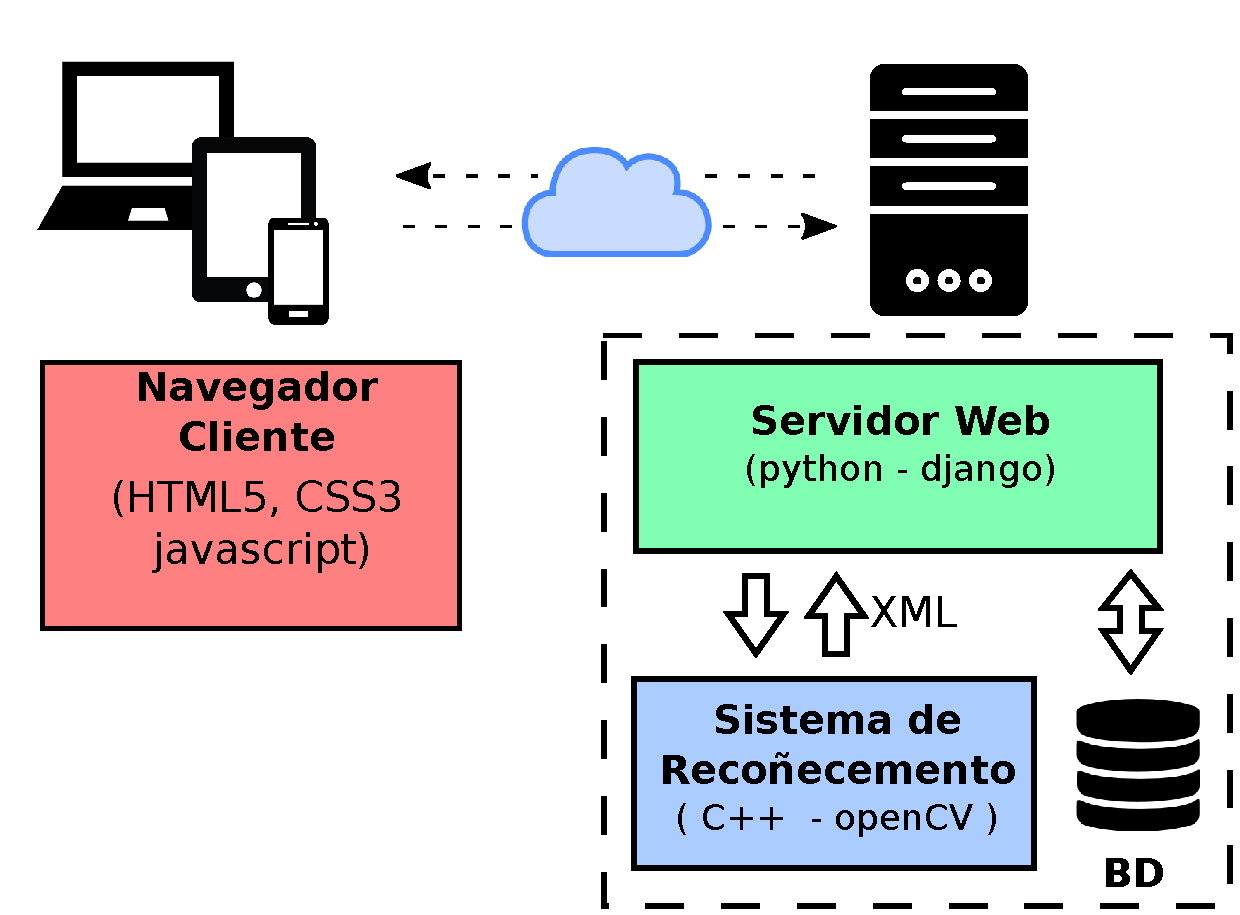
\includegraphics[scale=0.45]{figures/ArqSistemaSimplificado.pdf}
        \caption{Diagrama simplificado da Arquitectura do Sistema}
    \label{fig:ArqSistemaSimplificado}
    \end{center}
    \end{figure}
	
\section{Análise do comportamento}
	É un dos campos de investigación mas activos hoxe en día. A idea principal na que se 
	centran estes sistemas como o que nos ocupa é a de detectar calquera acción levada a 
	cabo polos obxectos involucrados nunha escena de vídeo. Un obxecto é calquera cousa 
	que debe ser seguida, polo que dependendo do tipo de problema estes obxectos poden 
	ser dunha natureza ou doutra.
	O tipo de accións a detectar tamén depende da tipoloxía do sistema, xa poden ser
	comportamentos individuais( camiñar, correr, loitar...) ou grupais (reunirse, abandonar
	un grupo de persoas...).
	
	Tanto neste proxecto como nos sistemas para a análise do comportamento en xeral, 
	pódense discernir tres tarefas importantes que colaboran entre si \cite{brais-thesis}:
	
	\begin{itemize}
	
		\item{\textbf{Detección de Obxectos:}}\label{cap:DeteccionObxetos} Partindo dunha secuencia de vídeo como 
		entrada obtéñense os distintos obxectos que aparecen en cada fotograma da escena.
		Para este fin empréganse técnicas de visión por computador.
		
		%Aqui podríame extender falando da Substracción de Fondo, o Fluxo Óptico e os Sistemas de alto Nivel
		
		\item{\textbf{Seguimento de Obxectos:}} A partires da información obtida na detección, asígnanselle 
		identificadores a cada obxecto detectado no vídeo, agrupando se procede distintos
		obxectos baixo o mesmo identificador en caso de considerarse que estes obxectos forman
		parte de un grupo ou unha mesma detección.
		
		% Aquí podría falar das aproximacións por apariencia, filtro de Kalman, filtro de Partículas ..
		
		\item{\textbf{Análise do comportamento de Alto Nivel:}} Unha vez obtida a información dos 
		dous pasos anteriores pódese catalogar o comportamento de cada detección empregando
		técnicas de recoñecemento de patróns.
	
	\end{itemize}	
	
	Os resultados máis destacables destas técnicas cos que a aplicación terá que traballar serán:
	\begin{itemize}
		\item A lista de obxectos detectados para cada un dos fotogramas e a súa posición neles
		\item A traxectoria de cada un dos obxectos detectados
		\item O grao de anormalidade da traxectoria seguida por un obxecto en cada un dos fotogramas
	\end{itemize}
	
	Estas tres tarefas agrúpanse baixo un mesmo sistema ao que chamaremos Sistema de Recoñecemento
	e que xunto co servidor web, apoiado nos fundamentos que veremos a continuación, forman o lado
	servidor deste proxecto. 
	
\section{Programación Web}

	A programación web de aplicacións de carácter empresarial require do coñecemento da rede, ademais
	do de unha serie de ferramentas e estratexias para chegar a un deseño sostible e de calidade.
	
	A arquitectura clásica das aplicacións web pódese ver no gráfico \ref{fig:ArquitecturaAppWeb}, 
	ela contén unha parte cliente que se executa no navegador do usuario, e unha parte servidor que
	á súa vez acostuma a dividirse nunha BD (Base de Datos) que almacena a información precisa, unha 
	capa modelo que reflexa o modelo de negocio da nosa aplicación tipicamente nalgunha linguaxe 
	de programación e por último unha capa de IU Web (Interface de Usuario Web) que se encarga de 
	transformar os datos da capa modelo a un formato web comprensible polo cliente e viceversa.
	
	\begin{figure}[htp]
	\begin{center}
		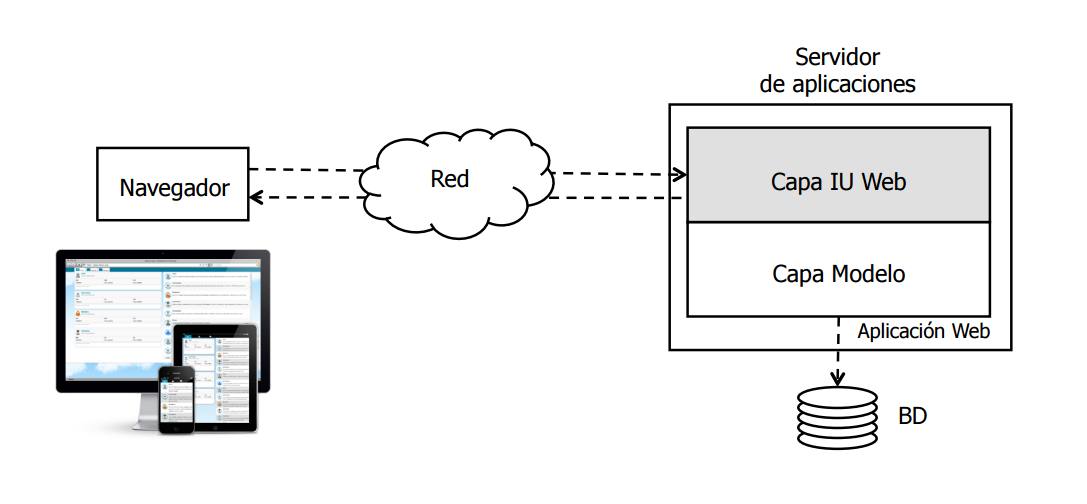
\includegraphics[scale=0.35]{figures/ArquitecturaAppWeb.png}
		\caption{Clásica arquitectura dunha aplicación web empresarial}
	\label{fig:ArquitecturaAppWeb}
	\end{center}
	\end{figure}

	As técnicas e estratexias máis importantes á hora de construír unha aplicación web relátanse nos
	puntos subseguistes:
	
	\subsection {Desenvolvemento Áxil}
		Para reducir custos e poder proporcionar solucións rápidas é preciso que as 
		aplicacións web's de carácter empresarial se leven a cabo en pouco tempo e con
		bos principios de enxeñaría, a isto contribúen en gran medida as estratexias de programación 
		que se explican a continuación e que se ven no diagrama \ref{fig:fundamentos}.
		
    \begin{figure}[htp]
    \begin{center}
        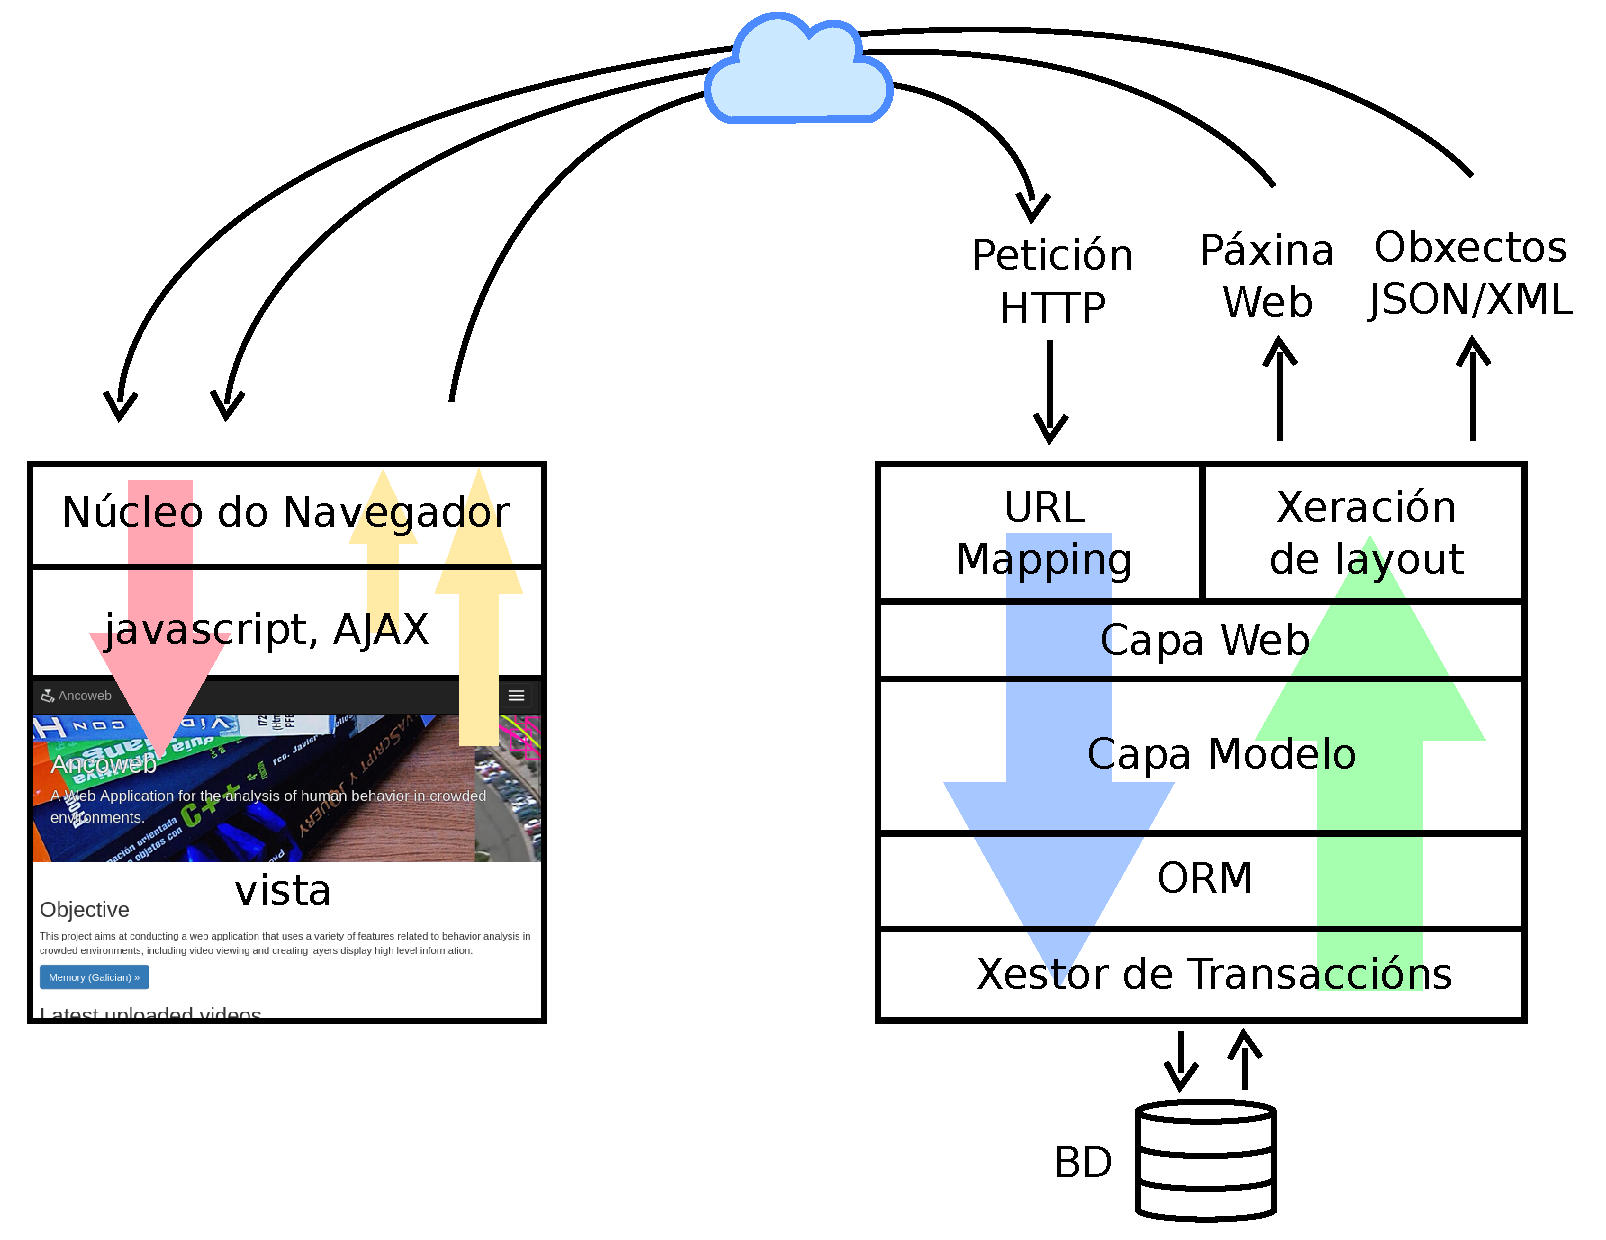
\includegraphics[scale=0.4]{figures/fundamentos.pdf}
        \caption{Diagrama sobre os conceptos de programación}
    \label{fig:fundamentos}
    \end{center}
    \end{figure}
		
        \subsubsection{Soporte para transaccións}
            Unha transacción nun Sistema Xestor de Base de Datos (SGBD) é un conxunto de ordes que
            se executan formando unha unidade de traballo, de forma invisible e atómica. 
            As transaccións cobran gran importancia nas aplicacións web debido á inestabilidade 
            da rede e á concorrencia dos distintos clientes conectados, polo que é axuda a un 
            desenvolvemento moi áxil que a tecnoloxía traia a súa xestión integrada.
        
        \subsubsection{Object-Relational Mapping (ORM)}
            Os mapeado obxecto-relación é unha das técnicas de programación que máis velocidade imprimen
            na construción de web's, xa que converte os datos dunha linguaxe Orientada a Obxectos (OO) a 
            datos de un sistema relacional no que son persistidos e viceversa, aforrando ao programador
            o traballo de ter que programar o código para esta tarefa. É desexable pois que a tecnoloxía
            a empregar dispoña dun mapeador obxecto-relacional ben integrado, algúns exemplos disto poden
            ser: a combinación Java+Maven+Hibernate, o EF(Entity Framework) de Microsoft ou os 
            Models de Django.
        
        \subsubsection{Xestión de Layout}
            Tamén resulta moi practico dispoñer dunha linguaxe de plantilla que permitan xerar contido
            HTML ben estruturado dinamicamente. Algúns exemplos son o Sistema de Templates de Django, o 
            Sistema JSP de Spring, a libraría Thymeleaf ou os compoñentes de ASP.NET. Todos eles axudan 
            a xerar contido HTML de xeito sinxelo e escalable que logo será enviado ao cliente. De
            tódolos xeitos esta parte cliente as veces precisa comunicarse co servidor sen que sexa 
            preciso unha recarga da páxina e para elo empregase AJAX.
		
    \subsection{AJAX}
		AJAX ou Asynchronous JavaScript And XML é unha tecnoloxía da web empregada para crear 
		aplicacións interactivas, estas aplicacións execútanse no navegador dos usuarios mentres 
		manteñen unha comunicación asíncrona co lado servidor en segundo plano. Normalmente 
		empregase javascript coma linguaxe para a realización das chamadas asíncronas en combinación
		con algunha linguaxe para a definición de obxectos como XML ou JSON, para as que ademais os
		propios navegadores adoitan a facilitar ferramentas de parsing.
		
	\subsection{Outras cuestións da web}
		A maiores existe toda unha gama de outras funcionalidades que cobran importancia cando deseñamos
		e construímos unha web como o manexo de erros nos formularios, internacionalización (i18n), 
		visualización de grande cantidades de datos (en listas ou táboas), seguridade...
		
		
\section{O Vídeo}
    O vídeo permite gravar, procesar, almacenar e transmitir información en forma de 
    imaxe en movemento, esta imaxe en movemento soe estar composta por unha serie de imaxes 
    estáticas chamadas fotogramas, que se manexan a unha velocidade alta causando o efecto de que o
    que se está a ver está en movemento.
    
    Non obstante o vídeo en formato electrónico non almacena necesariamente todas as imaxes de forma
    individual xa que isto suporía moita información redundante. En lugar disto empréganse técnicas
    de codificación-decodificación (codec's) que comprimen e descomprimen os datos para facilitar o
    seu manexo.

    \subsection{Codec's}
        Os codec's teñen como función principal a de transformar unha sinal de vídeo para que poida
        ser visto. A maioría dos codec's provocan con cada transformación unha perda de información
        para conseguir un tamaño final o máis pequeno posible, estes codec's chámanse lossless (con 
        perdida) e a pesares de que perden calidade soe compensar pola cantidade de espazo que 
        aforran ao comprimilo vídeo.
        
        A parte de este fenómeno da compresión tamén cobra moita importancia outros aspectos 
        relacionados co vídeo como a reprodución e sincronización de son, os subtítulos do vídeo,
        as imaxes representativas deste... Todo isto depende do formato no que se almacene o vídeo.
        
    \subsection{Formato de Vídeo}
        O formato dun vídeo determina como se almacenan os distintos tipos de información involucrada
        como as imaxes que poden estar codificadas en varios codec, o son, os subtítulos...
        este formato correspondese cunha extensión específica do arquivo que o contén, como por 
        exemplo:
        
        \begin{itemize}
        \item \textbf{AVI (Audio Video Interleaved):} 
            Sendo un dos formatos máis famosos pode conter un vídeo dunha calidade excelente pero
            soe requirir dunha gran capacidade. Os codec's que se soen empregar neste formato pola 
            súa capacidade de compresión e calidade aceptable son DivX e XviD, inda que tamén se 
            permiten outros como DV(Digital Video), CinePak... 
            
        \item \textbf{MKV (Matroska):}
            É un formato de código aberto que basea o seu nome nas clásicas bonecas Matrioskas. Ten
            capacidade para conter tanto vídeo, son e subtítulos en diferentes idiomas, empregándose
            como códec de vídeo normalmente algunha implementación de H.264, como por exemplo x264. 
            Mentres que para o son é habitual empregar o codec de audio Vorbis.

        \item \textbf{ WebM (Google, 2010):}
            Un dos formatos máis recentes é o WebM (WebMovie), un proxecto lixeiramente baseado en 
            Matroska adquirido e liberalizado por Google en 2010 co obxectivo de empregalo con HTML5
            como estándar libre. O formato ten un excelente rendemento e xunto ao codec VP9, motivo
            polo cal forma parte dos recomendados pola W3C.
            
        \item \textbf{Formato OGG (Xiph.Org, 1993):} 
            O formato contedor OGG é un formato libre deseñado para incluír vídeo, son, 
            subtítulos e metadatos. O vídeo en este formato soe estar codificado co codec Theora, 
            que se basea nunha versión liberada de VP3. Tamén se emprega para este tipo de 
            empaquetado a extensión .OGV, mais o que marca o estándar é a extensión .OGG.  
            
        \item \textbf{MP4 - MPEG (Moving Pictures Expert Group):}
        
        O  Moving Picture Experts Group (MPEG) é un grupo de expertos da ISO (Organización 
        Internacional de Normalización) e da Comisión Electrotécnica Internacional (IEC) para
        crear estándares en canto ao mundo do audio e o vídeo.
        
        Froito do traballo deste grupo naceron os formatos MPEG-1 (calidade CD), MPEG-2 (calidade 
        DVD), MPEG-3 (orientado ao audio MP3) e MPEG-4 que é o que máis nos interesa xa que vai 
        enfocado á compresión de vídeo e son na web, podendo incluír tamén subtítulos ou imaxes de 
        referencia. O ficheiros de este último formato teñen extensión .mp4.

        \end{itemize}


    \subsection{Streaming de Vídeo}
        Dado que este proxecto está centrado no tratamento de vídeo, é de especial importancia ver 
        de que xeitos podemos distribuílo e reproducilo a través da rede. A estes efectos existen dúas
        grandes alternativas que varían en canto ao seu grao de escalabilidade, dificultade de 
        implementación, e calidade final do servizo:
        
        \subsubsection{Pseudo Streaming ou Descarga Progresiva}
            Consiste na descarga do vídeo por fragmentos, tipicamente empregando o protocolo HTTP. 
            Neste formato, o reprodutor vai acumulando fragmentos de vídeo ata obter os precisos como 
            para comezar a reprodución, mais se o ancho de banda fose insuficiente, o vídeo remataría
            por pararse. Este sistema é o empregado por servizos como YouTube, Vimeo, DailyMotion...
            
            Será a opción empregada por motivos de simplicidade, mais compre explicar tamén o verdadeiro 
            Streaming, xa que é a diferenza do pseudo-streaming pode ser empregado para a emisión de
            contido en directo como o dunha cámara de seguridade.
            
        \subsubsection{Streaming}
        \label{sec:streaming}
            O verdadeiro streaming ( do inglés True Streaming) consiste na emisión en directo do 
            contido multimedia a través da rede, que o reprodutor reproduce no momento que recibe.
            Este outro xeito de distribuír vídeo, apoiase en axustar a calidade do vídeo ao ancho de
            banda do que dispón o cliente, evitando así interrupcións na reprodución.
            
            O protocolo máis destacable á hora de empregar este tipo de streaming é RTSP (Real-Time
            Streaming Protocol) que operando a nivel de aplicación permite controlar un ou varios fluxos 
            sincronizados de contido multimedia como se pode ver na figura \ref{fig:RTPS-diagram}.
            
            Por unha parte RTSP soe empregar o Real-Time Transport Protocol (RTP) sobre UDP(User 
            Datagram Protocol) para o transporte de contido multimedia, maximizando así o emprego 
            da rede pero sen garantir un mínimo na calidade do servizo.
            
            E por outra parte RTSP emprega o Real-time Control Protocol (RTCP) sobre TCP(Transmission 
            Control Protocol) para a transmisión periódica de paquetes de control da sesión, o
            diagnóstico de fallos e o control de la calidade da transmisión.
            
            \begin{figure}[htp]
            \begin{center}
                
\includegraphics[scale=0.6]{figures/RTPS-diagram.png}
                \caption{Diagrama conexión RTPS}
            \label{fig:RTPS-diagram}
            \end{center}
            \end{figure}
            
            RTSP asemellase a HTTP no formato das peticións/repostas e na sintaxe, pero dispoñendo 
            dun estado que permite tanto a clientes como a servidores facer peticións.

            Tamén existen outros protocolos propietarios como MMS (Microsoft Media Server)ou RTMP 
            (Real-Time Messaging Protocol) e RTMFP (Real-Time Media Flow Protocol) de Adobe.
            
\chapter{Análise de antecedentes e alternativas}
    En canto aos produtos existentes ate o momento que traballan no ámbito da detección de obxectos
    e a análise do comportamento, hai que diferenciar aqueles produtos da empresa
    privada que prometen grandes resultados pero dos cales debido á falta de medios non se pode 
    comprobar o seu correcto funcionamento, daqueles que pertencen ao mundo do software libre ou que
    están apoiados en documentos científicos e que si teñen unha reputación contrastada.
    
    
    \section{Software de carácter privativo}
    
        Do primeiro grupo pódese salientar toda unha serie de ferramentas que permiten o tratamento de 
        distintas señais de vídeo procedentes de varias cámaras sobre as que se executa unha análise que
        dependendo do producto ofrecenos uns datos ou outros. Algúns exemplos de estes productos son:
        
        \begin{itemize}
        \item \textbf{CyeWeb:}\cite{CyeWeb}
            É unha aplicación de escritorio para monitorización de cámaras de vixilancia que segundo 
            detallan na súa páxina web permite detección de movemento, conteo de obxectos, detección de
            aparcamentos en zoas non permitidas, detección de obxectos conflitivos...
            
        \item \textbf{Cerebrus Intelligent Video Analytics:}\cite{adventura-cerebrus-intelligent-video-analytics}
            Outra aplicación de escritorio que tamén obtén en directo o vídeo de varias cámaras de 
            vixilancia e mostra sobre este vídeo unha análise de alto nivel capaz de detectar intrusos,
            monitorizar de vehículos, detectar obxectos abandonados, contar persoas, etc.
        \end{itemize}
        
        En software privativo pero máis enfocados cara o tema da análise de comportamento e menos
        focalizados como programas de video-vixilancia temos outra serie de produtos como poden ser:
        
        \begin{itemize}
        \item  \textbf{Nolus:}\cite{nolus-human-behaviour}
            Dende esta empresa aseguran que o seu software é capaz de recoñecer distintos patróns de 
            comportamento en seres humanos e en animais.
        
        \item \textbf{WINanalyze:}\cite{WINanalyze-web-page}
            WINanalyze é unha aplicación de escritorio para a análise de vídeo procedente tanto de 
            cámaras en vivo como de ficheiros, que permite analizar os movementos realizados por un 
            obxecto do que se seguen distintos puntos de interese. Está baseado nunha serie de artigos
            científicos de comezos dos anos noventa sobre o seguimento de pixeles e puntos de interese
            que se poden consultar na web da empresa á que pertence\cite{mikromak-publications}.
        
        \item \textbf{Huygens Software - ObjectTracker:}\cite{Huygens-ObjectTracker}
            Huygens Software Suite é un conxunto de paquetes para o procesamento de imaxes.
            Esta suite centrada na análise de partículas inclúe funcionalidades como análise interactivo,
            visualización de volumes en 2D e 3D, funcionalidades para tratamento de imaxes procedentes
            de microscopio ou no tracking de obxectos mediante fluxo óptico: estudo das posicións,
            traxectorias, velocidades ...
            
        \end{itemize}

    \section{Software libre}
    \label{sec:video-vixilancia-libre}
        En este apartado ao igual que no anterior analizamos dous tipos de software, que non están
        intrinsecamente ligados entre si, senón que parece seguir liñas un pouco independentes. Por
        un lado están os programas de vídeo-vixilancia que implementan algún tipo de análise do
        comportamento e por outro lado as aplicacións para investigación científica que permiten 
        detectar comportamento e estudalo mais en detalle.
        
        Do primeiro grupo podemos destacar:
        \begin{itemize}
         \item \textbf{iSpy:}\cite{iSpy-webpage}
            iSpy é un dos software's libres para vídeo-vixilancia máis completos do mercado. Emprega
            unha arquitectura moi semellante á que se precisa neste traballo fin de grao, cun 
            servidor que recolle os sinais de vídeo para logo ofrecelas mediante un acceso web 
            dende calquera navegador. 
            Ao ser un proxecto de código libre sempre é posíbel descargalo para realizar sobre el as
            modificacións relativas á análise do comportamento, mais isto non é preciso posto que 
            dispón da posibilidade de acoplar plugins que modifican ou amplían o seu comportamento.
            Son de especial interese os plugins dispoñibles para realizar tarefas de visión por
            computador\cite{iSpy-plugins}, como poden ser detección e seguimento de actividades,
            recoñecemento de matriculas, conteo de persoas, detección de caras ou análise do 
            comportamento.
         \item \textbf{ZoneMinder:} \cite{zoneMinder-webPage}
            ZoneMinder é xunto con iSpy un dos software's de vídeo-vixilancia libres máis completo
            e potente proporcionando toda unha serie de funcionalidades para amosar vídeo de cámaras
            IP, de circuíto de televisión ou USB. Segue ao igual que iSpy unha arquitectura 
            cliente-servidor, e inda que non ten un abanico de plugins tan rico como o de iSpy 
            dispón de Detección de Movemento integrado\cite{zoneMinder-motion-detection}.
        \end{itemize}
        
        En outra liña diferente, tamén son de interese proxectos de carácter máis investigador que 
        permiten análise do comportamento como son:
        
        \begin{itemize}
         \item \textbf{SwisTrack:}\cite{SwisTrack-webPage}
            SwisTrack é unha ferramenta incriblemente versátil para o seguimento de obxectos, 
            animais, humanos... empregando como fonte de datos unha cámara ou ben un arquivo de 
            vídeo. Distribúese como unha aplicación de escritorio escrita en C++, e que emprega as 
            funcionalidades de OpenCV.
            É de destacar unha opción que permite acceder aos datos da súa análise vía web. O 
            programa dispón dunha interface TCP(Transmission Control Protocol), que amosa en formato
            \underline{text-based NMEA 0183 protocol} o resultado dos compoñentes de saída que 
            escriban nela.
            
         \item \textbf{Community Core Vision:}\cite{ccv-webPage}
            É un proxecto moi similar a SwisTrack, con algo menos de transcendencia pero con 
            soporte multiplataforma, tamén creado como interface de escritorio permite escoller 
            entre 27 opcións de análise diferentes para o tratamento do vídeo.
            
        \item \textbf{Seguimento de Insectos ou partículas:}
            Neste campo tamén son de especial utilidade os programas de tracking, de feito existen 
            dous destacables sistemas para a análise do comportamento dos insectos: BIO-TRACKING
            \cite{bio-tracking-webPage} e Ctrax\cite{ctrax-webPage}, ambos permiten unha detallada
            análise para determinar cales son os comportamentos destes animais en función das
            traxectorias que seguen no seu camiño ou as zoas que máis frecuentan dentro dun
            determinado entorno.
        \end{itemize}

\chapter{Metodoloxía seguida no desenvolvemento de Proxecto}

Os diferentes obxectivos do proxecto abordáronse seguindo a Metodoloxía SCRUM, adaptada a
un proxecto de un único Developer.

Esta metodoloxía áxil tamén chamada melé pola súa inspiración no Rugby, permite un
desenvolvemento rápido en situacións de requisitos inestables. Apoiase no seu carácter 
iterativo e incremental, dividindo o traballo a realizar en períodos de aproximadamente un mes
chamados Sprint's.

Para a realización deste traballo de fin de grao foi preciso adaptala, pois está pensada en 
principio para organizar equipos de entre 3 a 9 persoas (Team) mentres que neste caso só se contará 
cunha única persoa para desenvolver todo o proxecto. Por outro lado, o marco de 
traballo planifica reunións diarias (Daily Scrum), ao supoñer que todos os membros do equipo 
traballan unha xornada laboral enteira entre cada unha destas reunións, o cal tampouco se dá 
no caso deste proxecto, xa que a dedicación será de determinadas horas nos momentos dispoñibles.

\section{As metodoloxías áxiles}
    Escolleuse unha metodoloxía áxil como SCRUM para este proxecto xa que as metodoloxías áxiles en
    xeral son unha forma excepcional de minimizar os riscos asociados grazas ao seu carácter 
    iterativo (abordase por iteracións curtas de tempo) e incremental(as funcionalidades do proxecto
    crecen en cada iteración). Este carácter obriga a levar a cabo as fases de planificación, análise 
    de requisitos, deseño, codificación, revisión e documentación en cada Sprint, o cal se se 
    compara coas metodoloxías clásicas fai que tras un Sprint se poida axustar o seguinte en función
    de todo o aprendido, sen a necesidade dunha longa experiencia para poder planificar con 
    exactitude.
    
    Outra faceta importante das metodoloxías áxiles é a falta de documentación, isto está motivado 
    polos sucesivos cambios que se producen nestes proxectos por mor do seu carácter adaptativo, e 
    que serían moito máis custosos se ademais de modificar o propio software fose preciso modificar
    longas listas de documentación asociada. Por este motivo, neste sistema: a análise de requisitos 
    plasmarase como unha lista de tarefas que pasan ao Sprint Backlog, os diagramas de deseño só se 
    elaborarán para as partes máis críticas do sistema, no código evitaranse comentarios 
    innecesarios e o plan de probas realizarase empregando unha folla excel en vez de un extenso 
    documento de texto.


\section{Persoas}

    Os tres papeis que se definen nesta metodoloxía \cite{la-guia-de-scrum} foron 
    adaptados do seguinte xeito:

    \subsection{ProductOwner}
        O papel de ProductOwner, que define os requisitos da aplicación estivo representado 
        polo director de proxecto Brais Cancela, que participou na creación do Anteproxecto.
        En certos momentos o señor Cancela tamén desempeñou a función de membro do equipo, 
        posto que é foi autor do algoritmo de análise de vídeo. 

    \subsection{ScrumMaster e Development Team}
        Ambos papeis leváronse a cabo polo autor, xa que carece de sentido definir ambas figuras
        nun equipo de unha única persoa. De este xeito á par que se desenvolvía o proxecto, íase
        asegurando o cumprimento das regras de SCRUM.
    
\section{Reunións}
As reunións pola súa parte modifícanse do seguinte xeito:

    \subsection{Sprint Planning Meeting}
        Esta reunión mantén o mesmo formato que no SCRUM orixinal, xuntando ao autor co	ProductOwner 
        e concretando as tarefas do Product Backlog que se realizarán no seguinte Sprint, pasando
        por tanto a formar parte do Sprint Backlog.
    
    \subsection{Daily Scrum}
        Dado que o equipo de Desenvolvemento e o ScrumMaster están conformados pola mesma persoa
        e que o número de horas diarias adicadas é moito menor que o de unha xornada laboral, considerouse
        oportuno substituír esta reunión diaria por unha reunión dúas veces á semana (Martes e Xoves 
        pola tarde normalmente). Na que se mostrase ao ProductOwner o avance do proxecto.
    
    \subsection{Sprint Review}
        Esta reunión fusionase co Sprint Planning Meeting, xa que ao mesmo tempo valorase o traballo
        realizado no Sprint que remata e, en base a el, planificase a videira iteración. 
    
    \subsection{Sprint Retrospective}
        Pola súa parte, esta reunión toma un carácter unipersoal, pasando a ser unha valoración do
        propio autor sobre as persoas, relacións, procesos e ferramentas implicadas no último Sprint.
        Nela avalíase os elementos con éxito e os suxeitos a melloras, creando un plan para implementar
        estas melloras na videira iteración.

\section{Control de Versións con GitHub}
    GitHub é un sistema de control de versións que permite a xestión dos distintos cambios
    efectuados sobre un produto software ou sobre a súa configuración. Facilitando a administración
    das distintas versións do produto. 
    
    GitHub tamén é unha plataforma de desenvolvemento colaborativo que emprega o sistema de
    control de versións Git. Escolleuse empregar este sistema pola súa potencia e simplicidade, xa
    que proporciona libre acceso aos titores para comprobar o avance do proxecto, e a súa vez asegura
    que o código este sempre ben seguro.
    
    A páxina do proxecto é: \url{https://github.com/iago-suarez/ancoweb-TFG} 
    
\section{Integración Continua con Travis CI}

    A Integración Continua (CI do inglés Continuous Integration) é un modelo informático que 
    consiste en facer integracións automáticas dun proxecto o máis a miúdo posible para así 
    poder detectar os posibles erros o antes posible, minimizando as súas posibles consecuencias.
    Outro factor importante é o feito de garantir que a versión subida ao repositorio segue a
    funcionar con independencia do entorno de desenvolvemento. Enténdense como pertencentes á 
    integración continua a compilación e a execución das probas de todo un proxecto.
    
    Travis CI é unha plataforma de integración continua para proxectos aloxados en GitHub, que 
    detecta automaticamente cando se produce un cambio no repositorio, e executa unha serie de pasos 
    definidos no ficheiro .travis.yml (figura \ref{fig:travisYml}), que contén as accións a realizar 
    antes, durante e tras a as probas.
    
    Escolleuse Travis CI, pola súa integración con GitHub, pola súa potencia (permite executar 
    practicamente todo o que se pode executar nunha máquina local) e pola súa sinxela integración
    con outras ferramentas como Coveralls.
    
    Pódese ver a páxina do proxecto en Travis CI en:\\ \url{https://travis-ci.org/iago-suarez/ancoweb-TFG}
    
    \begin{figure}[!htp]
    \begin{center}
        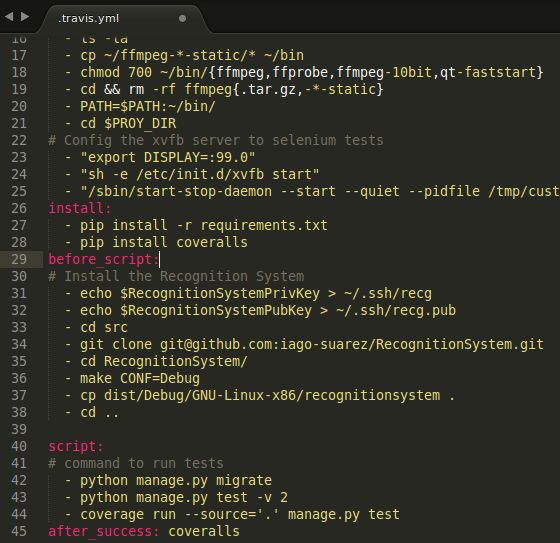
\includegraphics[scale=0.6]{figures/travisYml.png}
        \caption{Imaxe de parte do ficheiro .travis.yml}
    \label{fig:travisYml}
    \end{center}
    \end{figure}
    
    
\section{Control da cobertura con Coveralls}
    Coveralls é un servizo en liña que axuda a facer seguimento e control da cobertura de código para
    proxectos libres aloxados en GitHub. É tremendamente sinxelo de empregar e ademais está moi
    ben integrado con Travis CI, de xeito que cunha única liña de configuración pódese facer que o
    servidor de Travis CI envíe os resultados da cobertura a Coveralls cando as probas se pasen 
    correctamente.
    
    Neste proxecto empregarase nun comezo para facer seguimento dos test realizados sobre a parte 
    servidor inda que é posible que máis adiante se empregue tamén para probar o código que corre 
    na parte cliente.
    
    Pódese consultar a páxina de Coveralls para o proxecto en:\\
    \url{https://coveralls.io/github/iago-suarez/ancoweb-TFG}

\section{Xestión de Incidencias e Control de Proxecto con YouTrack}
    Co fin de levar a cabo un control das tarefas do Product Backlog e Sprint Backlog realizadas e 
    pendentes empregarase YouTrack como Sistema de Xestión de Incidencias (Issue Tracking System). 
    Un sistema de xestión de incidencias serve para xestionar as distintas incidencias (Tarefas 
    pendentes, Bug's, Problemas de usabilidade ou rendemento...) que poidan ter lugar nun entorno 
    como o proxecto web que nos ocupa. A estes efectos YouTrack mostrase como un completo sistema 
    de incidencias que permite a estimación e xestión de tempos, o emprego de comentarios para cada
    incidencia, buscas avanzadas, filtrado de incidencias, etc.
    
    Nótese que tamén se tiveron en conta outros sistemas de xestión de Incidencias como Redmine ou
    o sistema de xestión de incidencias integrado de GitHub, pero finalmente escolleuse YouTrack 
    pola súa coherencia coa filosofía áxil que se pode ver nos seus Paneis Áxiles, neles pódense
    xestionar todas as incidencias dun Sprint mediante o modelo Kanban, simplemente desprazando unha
    tarefa da columna de Tarefas Abertas á de Tarefas en Curso ou de esta última á de Tarefas 
    Solucionadas. A vista que YouTrack ofrece pódese ver na captura da figura \ref{fig:AgilePanel}.
    
    \begin{figure}[htp]
    \begin{center}
        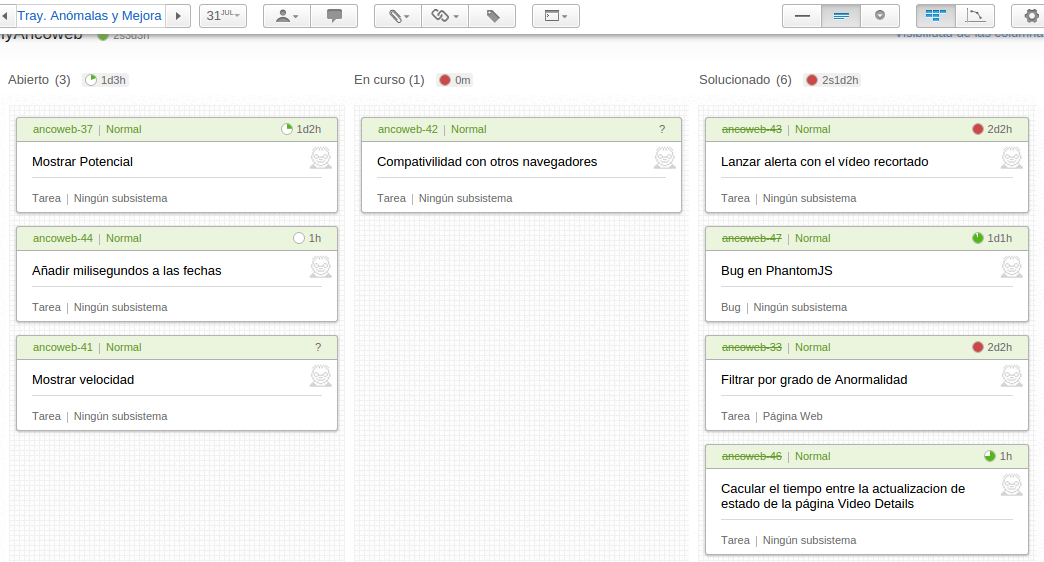
\includegraphics[scale=0.4]{figures/AgilePanel.png}
        \caption{Panel Áxil da ferramenta de xestión de incidencias YouTrack}
    \label{fig:AgilePanel}
    \end{center}
    \end{figure}
    
    Pódense consultar as incidencias do proxecto en YouTrack accedendo a:\\
    \url{http://iago-suarez.myjetbrains.com/youtrack/issues?q=*}
    
    


\chapter{Tecnoloxías Empregadas}
    
    O feito de traballar na web, e moito máis o de facelo no ámbito da análise de vídeo, requiren 
    que este sexa un proxecto cuns altos niveis de integración no que toman parte toda unha serie 
    de librerías e ferramentas software que axudan a alcanzar os fins desexado.
    
    Nesta primeiras sección procederase a explicar que tecnoloxías se tiveron en conta á hora de 
    escoller o xeito de implementar este proxecto e con que criterios, para a continuación proceder
    cunha explicación detallada de cada unha de elas. 
    
    \section{Estudo comparativo das tecnoloxías web}
    \label{sec:estudoTecnoloxias}
    Para a elaboración de este traballo de fin de grao, é preciso seleccionar unha serie de
    tecnoloxías tanto para o lado servidor coma para o lado cliente, vamos a empregar os seguintes
    criterios para poder comparalas entre si e escoller entre elas a que mellor se adecúan ás 
    necesidades do proxecto.

    \begin{itemize}

        \item {\textbf{Plataforma e Portabilidade\\}}
            Segundo as especificacións iniciais do proxecto, e de cara a facilitar a 
            implementación deste, as ferramentas empregadas deben de executarse baixo os
            Sistemas Operativos baseados en Linux.

        \item {\textbf{Compatibilidade co algoritmo de Procesado de Vídeo\\}}
            Dado que o algoritmo que procesa o vídeo foi parcialmente implementado en C++,
            a tecnoloxía que se empregue para o desenvolvemento da parte web debe dispoñer da
            máxima compatibilidade con esta linguaxe de programación.

        \item {\textbf{Desenvolvemento Áxil\\}}
            A tecnoloxía que se seleccione ten que minimizar o custe en tempo e esforzo da 
            implementación, por este motivo valorarase positivamente que dispoña de IDE's axeitados,
            facilidades de acceso a BD(Base de Datos),se é posible ORM(Object-Relational Mapping) 
            integrado, recarga en quente... En xeral todo aquelo que permita axilidade e flexibilidade.

    \end{itemize}

    Posto que empregamos unha arquitectura baseada no modelo cliente-servidor, temos que determinar 
    por un lado en que tecnoloxías vamos a construír o Servidor ou Back-End, e por outra parte o 
    Cliente ou Front-End que se executará nun navegador.  

    \subsection{Back-End}
        En canto ás tecnoloxías para a elaboración do Back-End, hai que ter en conta que procesará
        os datos proporcionados polo Front-End, atendendo as súas peticións e xestionando o modelo de 
        datos e os procesos implicados na aplicación. A maiores neste caso en concreto, o Back-End será
        o encargado de interactuar directamente co sistema de Análise de Vídeo.
        
        As tecnoloxías estudadas para esta parte do sistema son as seguintes:

        \subsubsection{Java}
        Java é unha das linguaxes máis empregadas actualmente. Ademais existen diversos
        frameworks web como Tapestry ou SpringMVC e en canto as BD Hibernate, que facilitan o 
        seu uso, mais é preciso integralos xa que non forman parte da plataforma en si. A súas 
        posibilidades de integración con C++ son altas grazas á interface JNI (Java Native 
        Interface), pero a súa configuración pódese volver tediosa. Un dos proxectos estudados
        para ver o seu funcionamento é Red5 \cite{red5-github-url}.
        
        \subsubsection{C\#}
        Esta linguaxe en combinación con .NET resulta unha combinación bastante áxil de cara
        á programación web, integrando na propia plataforma un deseñador Web e un ORM moi 
        intuitivo. O gran problema polo que se descartou este entorno foi polo seu baixo grao
        de compatibilidade cos sistemas operativos Linux.
        
        \subsubsection{C - C++}
        C++ presenta como era de esperar a maior compatibilidade co algoritmo implementado, non
        obstante, inda que existen algunhas utilidades que facilitan o desenvolvemento web con 
        esta linguaxe como Wt (Web Toolkit)\cite{wt-url}, o grado de axilidade está moi por 
        baixo do que facilitan o resto das combinacións. Tamén pode resultar de interese o
        coñecido proxecto Icecast\cite{icecast-url}, que fai streaming de vídeo sobre unha 
        interface web.
        
        \subsubsection{Python + Django}
        Python presentase como a mellor opción para desenvolver o lado servidor, por unha parte
        dispón do módulo Subprocess\cite{subprocess-module-url} que permite executar calquera
        comando pola terminal maximizando así a modularidade e a integración co algoritmo en C++.
        Por outra parte Django\cite{django-web-page-url} contén un potente ORM e un sistema de 
        ``Templates'' que simplifica a parte web. Para concluír cabe destacar o feito de que 
        Python sexa unha linguaxe interpretada, xa que isto evita o paso previo de compilación.
        
        
    \subsection{Front-End}
        Unha vez seleccionada a tecnoloxía do lado servidor, é hora de ver que opcións existen para
        o Front-End, a parte do Sistema encargada da interacción co usuario.
        
        Por unha parte están as tecnoloxías que pola súa transcendencia e nivel de aceptación
        considéranse xa imprescindibles no desenvolvemento web, estamos a falar de HTML e CSS linguaxes
        de facto para definir o contido e o aspecto visual respectivamente dunha páxina web.
        De estas linguaxes seleccionaremos as súas versións máis recentes, que a día de hoxe son HTML5 e
        CSS3.
        
        Sen embargo, noutros campos coma son a reprodución de vídeo e o control de elementos dinámicos
        non existe unha tecnoloxía que abarque a meirande parte da rede, é por elo que neste capítulo
        estudaremos aqueles xeitos que permitan a reprodución de vídeo e a maiores o debuxado de 
        figuras en movemento sobre este vídeo.\\
        
        En canto á reprodución de vídeo e o control deste destacan principalmente dúas alternativas:
        
        \subsubsection{Vídeo en Flash}
            Vídeo Flash é a tecnoloxía de reprodución de vídeo máis empregada e madura en
            internet dende hai anos. Inicialmente creada por Macromedia e mercada por Adobe 
            en 2005, permite crear elaboradas animacións vectoriais, que logo poden proxectarse
            sobre un vídeo, mentres que tamén manexa os eventos de reprodución de vídeo como o 
            play ou o stop.
            
            Ten certos problemas en tanto ao Posicionamento Web(SEO), reprodución en 
            dispositivos móbiles, accesibilidade... pero o meirande de todos eles é que mentres
            que outros dos exemplos estudados son 100\% libres, Flash é un programa propietario
            para o que é preciso adquirir unha licencia.        
            
        
        \subsubsection{Vídeo HTML5 + Javascript}
            Esta é outra das combinacións máis empregadas actualmente, xa que segue o estándar
            do W3C (World Wide Web Consortium)\cite{w3schools-video-tag} no que se define como se
            han de mostrar e obter os vídeos dunha páxina codificada coa linguaxe HTML5., e 
            destaca por seres extremadamente sinxelo en comparación con Flash ou outras tecnoloxías.
            
            Se o comparamos con Flash podemos ver a seguintes \textbf{vantaxes:}
            \begin{itemize}
                \item Resulta moito máis sinxelo de codificar grazas a que é o navegador o que se 
                encarga da reprodución do vídeo mentres que o programador só define o xeito de obtelo.
                \item Non precisa da instalación de ningún Plugin que poida dar problemas por exemplo 
                en dispositivos móbiles.
                \item Mentres que HTML5 e Javascript son libres, Flash é unha tecnoloxía propiedade de 
                Adobe.
                \item HTML5 + CSS3 dispón de máis facilidades se buscamos un deseño ``responsive''.
            \end{itemize}

            Será por tanto a alternativa escollida para a construción deste proxecto, e en canto ao 
            debuxo de figuras sobre o vídeo escolleremos o elemento $<canvas>$ tamén de HTML5. Todas
            estas tecnoloxías e moitas máis explícanse en detalle no seguinte capítulo.
            
    
    %%%%%%%%%%%%%%%%%%%%%%%%%%%%%%%%%%%%%%%%%%%%%%%%%%%%%%%%%%%%%%%%%%%%%%%%%%%%%%%%%%%%%%%%%%%%%%%
    
    
    A continuación explicase detidamente cal é a función de cada unha das tecnoloxías que forman 
    parte deste proxecto co fin de comprender o explicado nos capítulos seguintes. O diagrama 
    \ref{fig:ArqSistemaCustom} pode servir como orientación á hora de comprender que función 
    desempeña cada unha de elas.
    
    \begin{figure}[htp]
    \begin{center}
        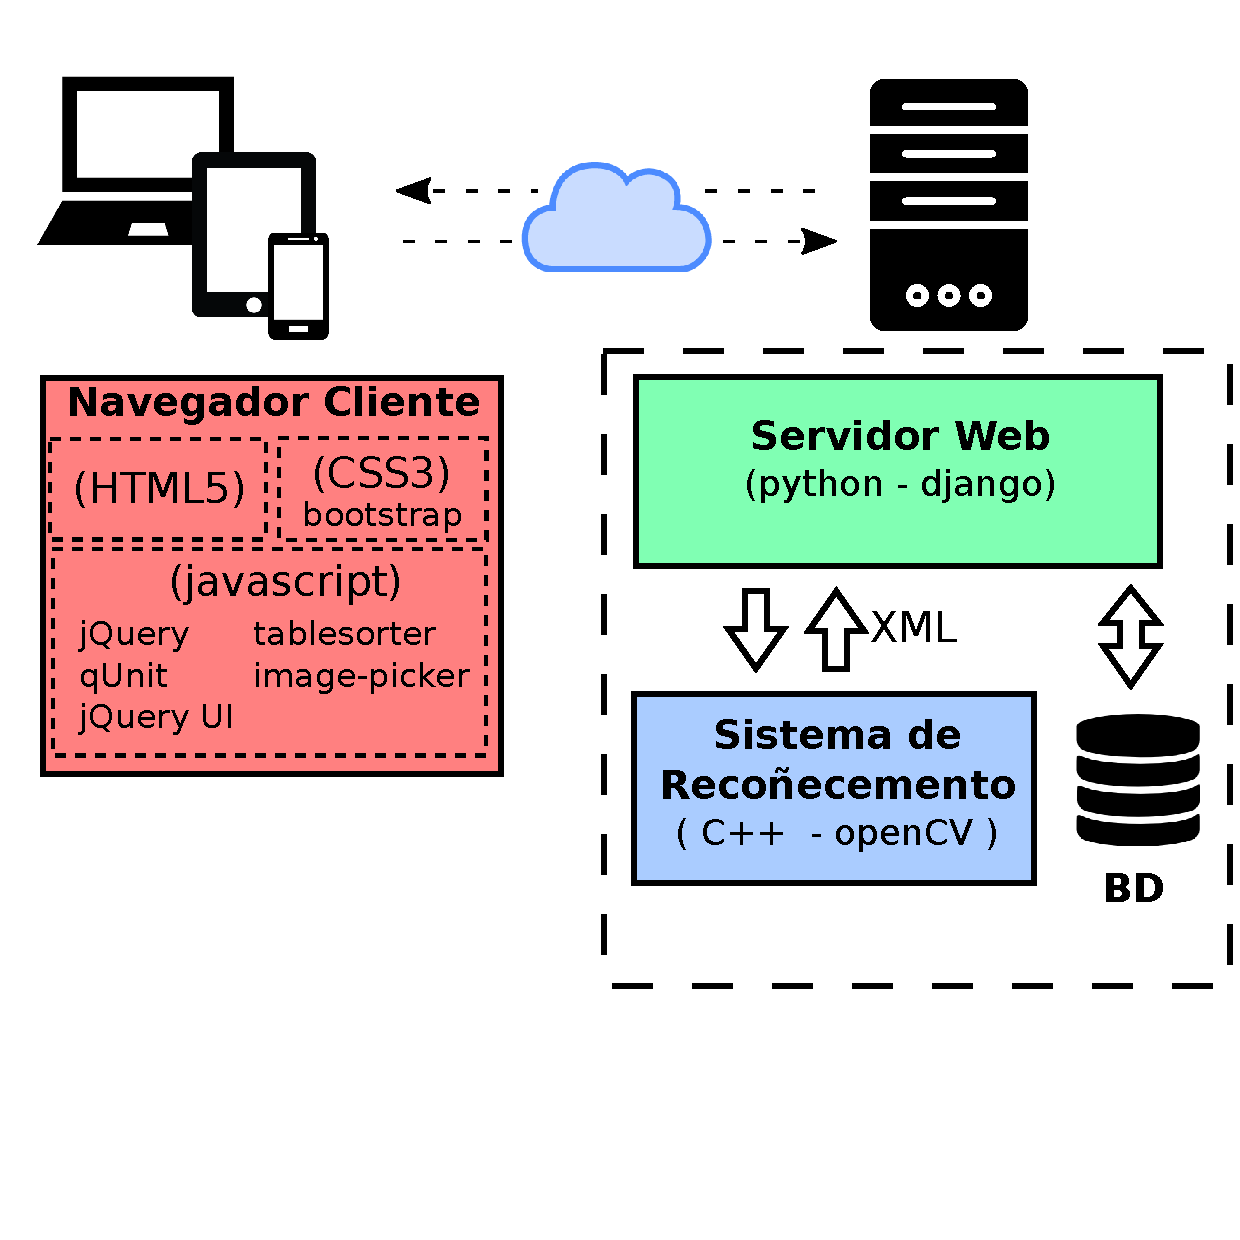
\includegraphics[scale=0.6]{figures/ArqSistemaCustom.pdf}
        \caption{Diagrama da Arquitectura do Sistema}
    \label{fig:ArqSistemaCustom}
    \end{center}
    \end{figure}
    
    Comezamos polas tecnoloxías empregadas no lado cliente:
    \section{Navegador Cliente}
    
    O navegador do cliente empregará unha serie de tecnoloxías para mostrar os datos obtidos do 
    servidor, as máis destacables son:
    
    \subsection{Estrutura da páxina: HTML5}
        Á hora de representar o contido dunha web precisase unha linguaxe que defina este contido,
        estruturándoo e facendo que sexa mais lexible e comprensible para que o navegador poida 
        representalo en pantalla, esta linguaxe é HTML.
        
        HTML (HyperText Markup Language) é a linguaxe de marcas empregada en internet para a elaboración
        de páxinas web, define unha estrutura básica e un código para a definición do contido da páxina
        como poden ser texto, imaxes, vídeos... Existen diversas versións deste estándar, mais para este
        proxecto empregarase a súa última versión HTML5, que inclúe toda unha serie de novos elementos.
        
        Un dos compoñentes que máis empregaremos para a construción desta web será o elemento 
        $<video>$ de HTML5 que achega unha serie de Métodos, Eventos e Propiedades
        \cite{w3school-video-events} que poden empregarse dende o código Javascript.
        
        A maiores do propio contido da páxina, HTML permite incluír referencias a outros ficheiros que 
        están tamén asociados á páxina como poden ser ficheiros javascript ou css que se mostran de 
        seguido.
    
    \subsection{Aplicando estilos visuais: CSS3}
        HTML permite unha perfecta estruturación dos elementos que compoñen unha páxina web, pero 
        en caso de que queiramos personalizar o estilo da páxina web, ou adaptala a diferentes 
        dispositivos precisamos CSS. CSS(Cascading Style Sheets) é unha linguaxe para definir e 
        crear a presentación dun documento HTML.
        
        Para elo defínense unha ou máis follas de estilos, que definen para cada elemento 
        seleccionado nelas unha serie de características de estilo. No caso da aplicación a 
        desenvolver a política de follas de estilo será a de crear unha folla de estilo xeral para 
        conter as características de estilo comúns a todo o proxecto e a maiores as que sexan 
        precisas para páxinas ou elementos concretos, todo elo traballando coa versión 3 desta linguaxe.
        
        \subsubsection{Estilo unificado: Twitter Bootstrap}
            CSS3 permite facer todos os axustes precisos en canto a estilo web, pero o problema é 
            que elaborar un bo estilo leva unha cantidade de tempo cuantiosa e por ese motivo se 
            precisa algunha libraría que marque unha pauta de estilo uniforme e que minimice o 
            traballo a realizar, bootstrap mostrase como unha das librarías mais empregadas a estes
            efectos e por iso foi seleccionada para este proxecto.
        
            Twitter bootstrap é un framework ou conxunto de ferramentas de código aberto para 
            deseñar web's. Contén todo un conxunto de plantillas como tipografía, botóns, formularios,
            táboas, barras de navegación... Estas plantillas normalmente consisten simplemente nun
            estilo CSS, pero ás veces tamén hai un procesado en javascript como o da función popover
            que permite xerar unha ventá flotante para amosar os datos dos obxectos detectados na 
            aplicación.
            
    \subsection{Execución de código no lado cliente: Javascript}
        A pesar de todas as cousas que permiten facer HTML e CSS moitas veces é preciso un 
        tratamento dinámico da información para desprazar un elemento na páxina, atender un evento
        clic, lazar unha ventá... e neste caso é preciso o emprego dunha linguaxe de scripting 
        como javascript.
    
        Javascript é a linguaxe de programación interpretada que se executa nos navegadores
        cumprindo co estándar ECMAScript, permite executar ordes podendo interactuar coa páxina 
        web a través da arbore DOM (Document Object Model) e co servidor mediante o sistema de
        chamadas asíncronas. Cada script en javascript está asociado a unha páxina web, de forma
        que todo o que executemos terá efecto sobre a páxina actual e nunca poderemos prolongar
        a execución dun código .js máis aló da vida desta páxina.\\
        
        A pesar de executarse nun navegador javascript é unha linguaxe cunha potencia 
        considerable, esta potencia ven da súa orientación a obxectos que tamén permite 
        programación imperativa con un tipado débil e dinámico.\\
        
        Javascript pode incluírse directamente no documento HTML, mais isto é problemático 
        porque mestura dúas linguaxes e non permite a reutilización do código javascript en
        distintas páxinas, polo que na practica sempre se traballará con código contido en
        ficheiros .js que logo serán importados dende as páxinas web que o precisen. Mediante 
        referencias tamén se pode engadir código de librarías, que pode achegarse de dous xeitos
        distintos, ou ben cun enlace á páxina onde están publicadas, ou ben descargando estas
        librerías ao servidor da aplicación e ofrecéndoas dende aí. O enfoque seguido neste 
        proxecto é o segundo, pois de este xeito a aplicación está auto-contida, podendo traballar
        sen conexión con internet, e mantendo sempre a integridade a pesar de que o provedor
        da biblioteca decida deixar de ofrecela.\\
        
        Mediante Javascript tamén pode manexarse o elemento $<canvas>$ de HTML5, que xera un mapa
        de bits para construír gráficos, manipular imaxes e crear dinamicamente animacións nunha
        páxina web. A única dúbida que soe xurdir sobre esta tecnoloxía está en canto ao seu 
        rendemento e alcance, pero exemplos como os que amosa Kevin Roast na súa páxina 
        web\cite{kevin-roast-canvas-examples} despexan toda dúbida posíbel.\\
        
        Por desgraza, a execución en navegador ten tamén os seus inconvenientes como a execución 
        multi-threading empregando \textbf{Web Workers}, estes elementos pensados para permitir
        a execución paralela de código javascript deixan polo de agora moito que desexar xa que 
        cada thread ten as súas propias variables estancas, impedindo polo tanto o acceso á 
        arbore DOM dende threads paralelos co problema engadido de que algúns navegadores como 
        Opera en vez de facer un multi-threading sobre threads do propio sistema  tan só simulan
        este fenómeno nun único thread. O paralelismo cobrará especial importancia 
        cando executemos os algoritmos que mostran os datos da análise en XML, pois ao 
        executarse todo no mesmo fío debemos prestar especial atención a non bloquear a 
        interface de usuario con tarefas moi prolongadas.\\
    
        \subsubsection{Simplificando javascript: jQuery}
    
            Javascript tamén é especialmente potente á hora de parsear documentos, xa sexa
            un documento HTML para acceder á arbore DOM ou ben un XML como o que xera o sistema de 
            análise. Por desgraza, o manexo de excepcións, e a selección de elementos dentro de un 
            documento son tarefas que se farán de forma moi habitual neste traballo e programar 
            estas tarefas con javascript resulta tremendamente laborioso, así que co fin de 
            simplificar esta tarefa empregarase a biblioteca jQuery.
                
            jQuery é unha biblioteca javascript pensada para simplificar os aspectos máis complexos desta 
            linguaxe como poden ser a manipulación de documentos HTML/XML ou as chamadas asíncronas 
            mediante AJAX. Está escrita en javascript e é 100\% libre, tal vez por isto sexa a biblioteca
            javascript máis empregada.
            
            O sistema de selección de jQuery é o mesmo que se emprega en CSS, permitindo seleccionar de 
            xeito sinxelo un conxunto de elementos dentro dun documento, a maiores tamén dispón de un 
            sinxelo acceso e modificación tantos destes elementos como dos seus atributos.
            
        \subsubsection{Probas no código javascript: Qunit}
        
            Outra faceta tamén moi laboriosa en javascript é a de probar o código escrito e xa que 
            a meirande parte desta aplicación estará escrita en javascript faise imprescindible 
            verificar que o código cumpre coa súa función. Por este motivo escolleuse outra 
            biblioteca tamén deseñada polo equipo de jQuery para simplificar os tests en javascript,
            esta biblioteca chamase Qunit.
            
            QUnit é un framework de probas unitarias para código javascript doado de empregar e bastante
            poderoso. Empregase tanto en jQuery, jQuery UI e os proxectos de jQuery Mobile sendo capaz 
            de probar calquera código javascript xenérico.
            
            Para facer probas emprega un conxunto de sentencias assert como todas as bibliotecas que 
            realizan tests de unidade. No caso da nosa aplicación empregarase para probar todo aquel
            código independente da arbore DOM da páxina. É importante destacar que co fin de maximizar
            a facilidade de proba do código na capa javascript seguíronse os consellos amosados na páxina
            de Qunit\cite{QunitMakeItTesteable} e unha interpretación flexible do MVC(Modelo 
            Vista Controlador) onde a vista está conformada polo código HTML+CSS, o controlador polo 
            manexadores dos ficheiros video-player.js, video-controls.js e por último as clases do 
            modelo en javascript nos ficheiros Detection.js, DetectionObserver.js, VideoDetections.js e 
            en menor medida suspicious-popup.js.
        
        \subsubsection{Creando un formulario con imaxes: Image-picker}
            Durante a construción da aplicación, nunha das páxinas xurdiu a necesidade de seccionar
            entre unha lista de imaxes, pero HTML5 é unha linguaxe que por unha parte permite
            amosar imaxes e por outro lado á hora de enviar información ao lado servidor permite 
            enviar datos moi simples mediante un formulario. Para dotar a HTML5 de esta 
            característica empregouse a libraría baseada en jQuery Image-Picker\cite{ImagePickerPage}
            que permite xerar un formulario cun campo de tipo ``select'' 
            baseado en imaxes en vez de nunha entrada despregable, todo elo de forma extremadamente
            sinxela.
        
        \subsubsection{Barras selectoras: jQuery UI}
        
            En outro momento da construción viuse a necesidade de engadir unha barra selectora para
            seleccionar un determinado valor na interface gráfica, e para elo optouse polo plugin 
            slider\cite{ComponenteSliderJqueryUi} da biblioteca jQuery UI. Esta biblioteca de 
            compoñentes para jQuery engádelle un conxunto de plugins, widgets e efectos visuais.
            Pódese descargar dende a súa páxina oficial o núcleo da biblioteca e os compoñentes 
            nos que se estea interesado.
        
        \subsubsection{Ordenar unha táboa: tablesorter}
        
            Como se verá mais adiante, os requirimentos da aplicación farán preciso que nunha das
            páxinas web's se amose unha táboa e que esta táboa se poida ordenar segundo o contido de
            distintas columnas. A estes efectos incorporase a derradeira libraría javascript chamada
            tablesorter\cite{tablesorter-webPage}. Tablesorter é un plugin baseado en jQuery para transformar 
            unha táboa HTML estándar coas etiquetas $<thead>$ e $<tbody>$ nunha táboa que se pode 
            ordenar polo contido das distintas columnas sen ter que recarga-la páxina. Neste
            caso será de moita utilidade á hora de amosar os resultados da análise, pois así 
            poderanse ordenar as deteccións segundo aparecen no vídeo, segundo o tempo que pasan 
            en pantalla... 
        
    Todas estas tecnoloxías de capa web axudarannos a mostrar con máis facilidade a análise que o
    sistema de recoñecemento faga do vídeo, e en canto as ferramentas empregadas para esta análise
    a ferramenta fundamental que se empregará é OpenCV.
    
\section{Sistema de Recoñecemento}
    O sistema de recoñecemento debe ser capaz de ler un vídeo e en base a el recoñecer os obxectos
    de ese vídeo á vez que analiza o seu comportamento. Isto pódese implementar de distintos xeitos,
    mais neste proxecto en concreto fíxose empregando a linguaxe de programación C++ que xa se citou
    na sección \ref{sec:estudoTecnoloxias}, en combinación coa librería OpenCV e a linguaxe de marcas
    XML.

\subsection{Análise do comportamento: OpenCV}
    
    OpenCV é unha biblioteca libre de visión artificial escrita en código C/C++ optimizado.
    Dende a súa aparición publicada por Intel en Xaneiro de 1999, empregouse en infinidade 
    de proxectos, tanto para detección de movemento como para aplicativos de control de procesos
    que requiren recoñecemento de obxectos.
    
    OpenCV é multiplataforma, existindo versión para GNU/Linux, Mac OS X e Windows. Contén máis 
    de 500 funcións que abarcan unha ampla gama de áreas como o proceso de visión, recoñecemento
    de obxectos (tamén recoñecemento facial), calibrado de cámaras, realidade aumentada e visión
    robótica.
    
    Por todas estas características OpenCV é unha das bibliotecas máis empregadas hoxe en día, e é
    por elo tamén que se escolleu para a implementación do sistema de recoñecemento que a aplicación
    web empregará para a análise do vídeo.
    
    Non obstante, xa que se desexa que a aplicación web sexa o máis versátil posible, contemplase a
    posibilidade de que poida empregar para a análise sistemas desenvoltos noutras tecnoloxías como
    pode ser Matlab. E para dotala deste grao de versatilidade decídese definir unha interface de
    liña de comando a través da cal se chamará ao sistema, e un formato de ficheiro XML (Extensible 
    Markup Language) no que este sistema de recoñecemento deben escribir os datos da súa análise.
        
\subsection{Como comunicar sistemas entre si: XML}
    
    Como os datos que devolve o sistema de recoñecemento teñen que ser gardados nun ficheiro de 
    xeito que calquera sistema poida entendelos ou traballar con eles, precisase un formato para
    ese ficheiro de saída que sexa capaz de almacenar datos estruturados de forma sinxela e 
    comprensible, este formato é XML(Extensible Markup Language).

    XML é unha linguaxe de marcas desenvolvida polo W3C (World Wide Web Consortium) e empregado
    para almacenar datos de forma clara e lexible. Permite definir a gramática de linguaxes 
    específicas para estruturar así grandes documentos.
    
    Os documentos XML seguen una estrutura xerárquica baseada en etiquetas(tag's) e atributos,
    que se poden definir nunha Definición de Tipo de Documento ou DTD. \cite{dtd-web-page}
    
    Cando un documento en formato XML segue as directrices definidas no ficheiro DTD asociado,
    dise que este ficheiro esta ben formado(well formed en inglés), e para validar iso empregarase
    na elaboración do traballo algún avaliador de XML en liña como por exemplo o da W3Chools.\cite{xml-validator}
    
    XML é especialmente útil para comunicar varias aplicacións que traballan en tecnoloxías 
    diferentes grazas á súa simplicidade que permite integrar os datos de xeito moi sinxelo. Precisamente
    por iso, servirá como nexo de unión entre o sistema de análise e a aplicación web. 
    
    Para a modificación da súa aparencia pódese empregar \emph{CSS3} (Follas de Estilos en 
    Cascada), e para modificar o seu comportamento, o elemento $<video>$ de HTML5 achega
    unha serie de Métodos, Eventos e Propiedades\cite{w3school-video-events} que poden
    empregarse dende código \emph{Javascript}.
    
\section{Servidor Web}
    Como se explicou anteriormente na sección \ref{sec:estudoTecnoloxias} Django é un framework
    que traballa sobre Python para a creación de páxinas web, as súas funcionalidades empregadas
    explicaranse pouco a pouco no capítulo \ref{cap:desenvolvemento}, polo que aquí explicaranse
    outros compoñentes do servidor empregados que compre coñecer antes de proseguir, en concreto 
    ffmpeg.
    
\subsection{Obter información do vídeo con FFmpeg}
    Ao tratarse a nosa aplicación dunha web centrada principalmente no traballo con vídeos, é 
    preciso dispor de unha ferramenta capaz de proporcionar datos sobre ese vídeo como poden ser 
    a súa duración, o seu número de fotogramas por segundo... e tamén capaz de transformar vídeo
    de un formato a outro. O software empregado para esta labor no proxecto é FFmpeg.

    FFmpeg é unha colección de software libre que pode gravar, converter (transcodificar) e facer
    streaming de audio e vídeo, nel está incluído libavcodec unha biblioteca de codecs que contén 
    aqueles máis empregados. Pódese dicir ademais de el que a pesar do seu grandioso número de 
    opcións é un programa bastante sinxelo de empregar.
    
\chapter{Desenvolvemento}
\label{cap:desenvolvemento}

\section{Funcionalidades desexadas}
    Antes de comezar o ciclo de sprint's tivo lugar unha pequena fase de análise no que se 
    requiriron as seguintes funcionalidades do proxecto a realizar:
    \begin{itemize}
     \item \textbf{Control de Usuarios:} É preciso un mínimo control de usuarios para controlar que
        sube vídeos á plataforma.
     \item \textbf{Carga de Vídeo:} Dado que a aplicación traballará con vídeos subidos polos 
        usuarios, o primeiro paso é lograr a subida exitosa de vídeos á plataforma por parte de
        usuarios autenticados.
     \item \textbf{Reprodución de Vídeo:} Desexase que a aplicación permita a reprodución dos vídeos
        contidos, mediante técnicas de streaming ou pseudo-streaming.
     \item \textbf{Lista de vídeos e Imaxe de Portada:} É preciso amosar de algún modo os vídeos 
        subidos á plataforma, a poder ser cunha imaxe representativa que axude a identificalos e con
        algún mecanismo de busca que permita filtralos en caso de que haxa un número elevado de eles.
     \item \textbf{Análise de Vídeo:} A aplicación web debe facer uso de dúas librerías de 
        computación visual proporcionadas polo laboratorio VARPA para analizar os vídeos subidos e
        extraer de eles os obxectos detectados e unha análise do seu comportamento, como é lóxico só
        os usuarios autenticados porán facer isto xa que só eles poden subir vídeos á aplicación.
     \item \textbf{Mostrar Deteccións:} Devénse amosar aqueles obxectos detectados mediante unha 
        capa de información extra sobre o vídeo subido. 
     \item \textbf{Traxectorias:} Tamén se han de indicar con unha capa de información sobre o vídeo
        as traxectorias seguidas polos obxectos detectados.
     \item \textbf{Listar Deteccións:} É importante listar os obxectos detectados en todo o vídeo coa
        súa información asociada, así como listar tamén aqueles que están en escena nun momento 
        determinado.
     \item \textbf{Detección do comportamento anómalo:} Desexase que empregando as funcionalidades
        da biblioteca proporcionada se analice o comportamento dos obxectos involucrados nunha 
        escena para así poder filtralos segundo o estraño que resulte este comportamento.
     \item \textbf{Popups de deteccións sospeitosas:} Outra funcionalidade requirida é que cando un
        obxecto teña un comportamento sospeitoso respecto ao do resto de obxectos, se abra unha nova
        ventá que o siga para poder ver mais de preto o que está a facer.
    \end{itemize}

O desenvolvemento da aplicación tivo lugar seguindo a filosofía de SCRUM, polo que o enfoque mais 
correcto neste caso para ver como se cumpriron todas as funcionalidades anteriores é o de explicar 
o traballo acometido en cada un dos sprints.
  
\section{v0.1 Cargar e Visualizar vídeos}
    Neste primeiro Sprint a parte de adicar moitas horas á formación no framework de Django e no 
    traballo con GitHub, creouse o esquema básico sobre o que se partirá para a creación e toda a
    web. Este esquema está baseado no plantilla Edge\cite{edge-templ}, que proporciona un control 
    mínimo de usuarios, unha liña de estilo, integración con bootstrap e control de administrador,
    inda que posteriormente a maioría destes aspectos tiveron que ser modificados ou ampliados.
    
    A partir desta plantilla que xa proporciona o control de usuarios, as dúas primeiras 
    funcionalidades a implementar foron a Carga dos vídeos e a súa reprodución.
    
    \subsection{Carga de Vídeo}
        Dado que a aplicación traballará con vídeos subidos polos usuarios, o primeiro paso é lograr
        a subida exitosa de vídeos á plataforma. Para este fin empregarase un formulario HTML que 
        viaxa sobre unha chamada POST de HTTP (figura \ref{fig:SubidaVideoForm}). 
        Cando o navegador faga esta chamada incluíndo o vídeo como parte do formulario, este vídeo
        comezará a subirse ao servidor en pequenos anaquiños (data chunk).
        
        \begin{figure}[htp]
        \begin{center}
            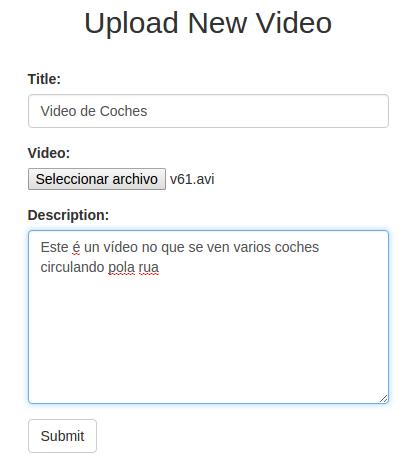
\includegraphics[scale=0.6]{figures/SubidaVideoForm.png}
            \caption{Formulario para a creación de vídeos}
        \label{fig:SubidaVideoForm}
        \end{center}
        \end{figure}    
        
        É de especial importancia que no caso de que o vídeo teña un peso considerable e precise 
        duns cantos segundos para subirse á plataforma, o usuario poida coñecer de forma gráfica
        o avance deste proceso.
        
        Con este fin, crease un sistema de notificación de progreso baseado no 
        django-progressbarupload \cite{django-progressbarupload}, este sistema apoiase nunha compoñente
        fundamental chamada VideoUploadHandler, que é unha extensión da interface de Django 
        TemporaryFileUploadHandler \cite{TemporaryFileUploadHandler}, e que basicamente manexa a subida
        dun ficheiro de tamaño considerable.\\
        
        Esta compoñente componse dunha función de inicio (handle\_raw\_input) que crea unha entrada 
        na Cache de Django, almacenando como chave un número aleatorio e a IP do cliente que está a
        subir o vídeo, e como valor o tamaño do ficheiro e o porcentaxe de este que xa está subido.
        Esta entrada será actualizada cada vez que o servidor reciba un novo anaco de vídeo (mediante
        a outra función do compoñente VideoUploadHandler, receive\_data\_chunk). 
        
        Por outra parte, para que visualmente o cliente poida ver o avance da subida a través unha
        barra de progreso, crease unha función asíncrona en javascript (Tecnoloxía AJAX), que 
        periodicamente consulta ao servidor para obter o valor da cache que indica a porcentaxe de
        subida do vídeo, e unha vez obtido, actualiza a barra de progreso para mostralo. Todo isto
        ten lugar no navegador mentres este inda está a subir o arquivo de vídeo.

        Unha vez que a subida se completa, o POST é manexado pola vista UploadView, que se todos
        os datos do formulario son correctos, encargase de crear un modelo VideoModel. Como parte
        desta creación o vídeo pasa do directorio temporal no que foi almacenado (baixo linux por 
        defecto é /tmp) a un directorio calculado pola función get\_valid\_filename. Esta función
        pásaselle ao modelo como parte do seu campo ''video'' do tipo FileField. Todo este proceso
        pódese ver de xeito mais claro no diagrama \ref{fig:SubidaVideo1} e \ref{fig:SubidaVideo2}.
        
        \begin{figure}[htp]
        \begin{center}
            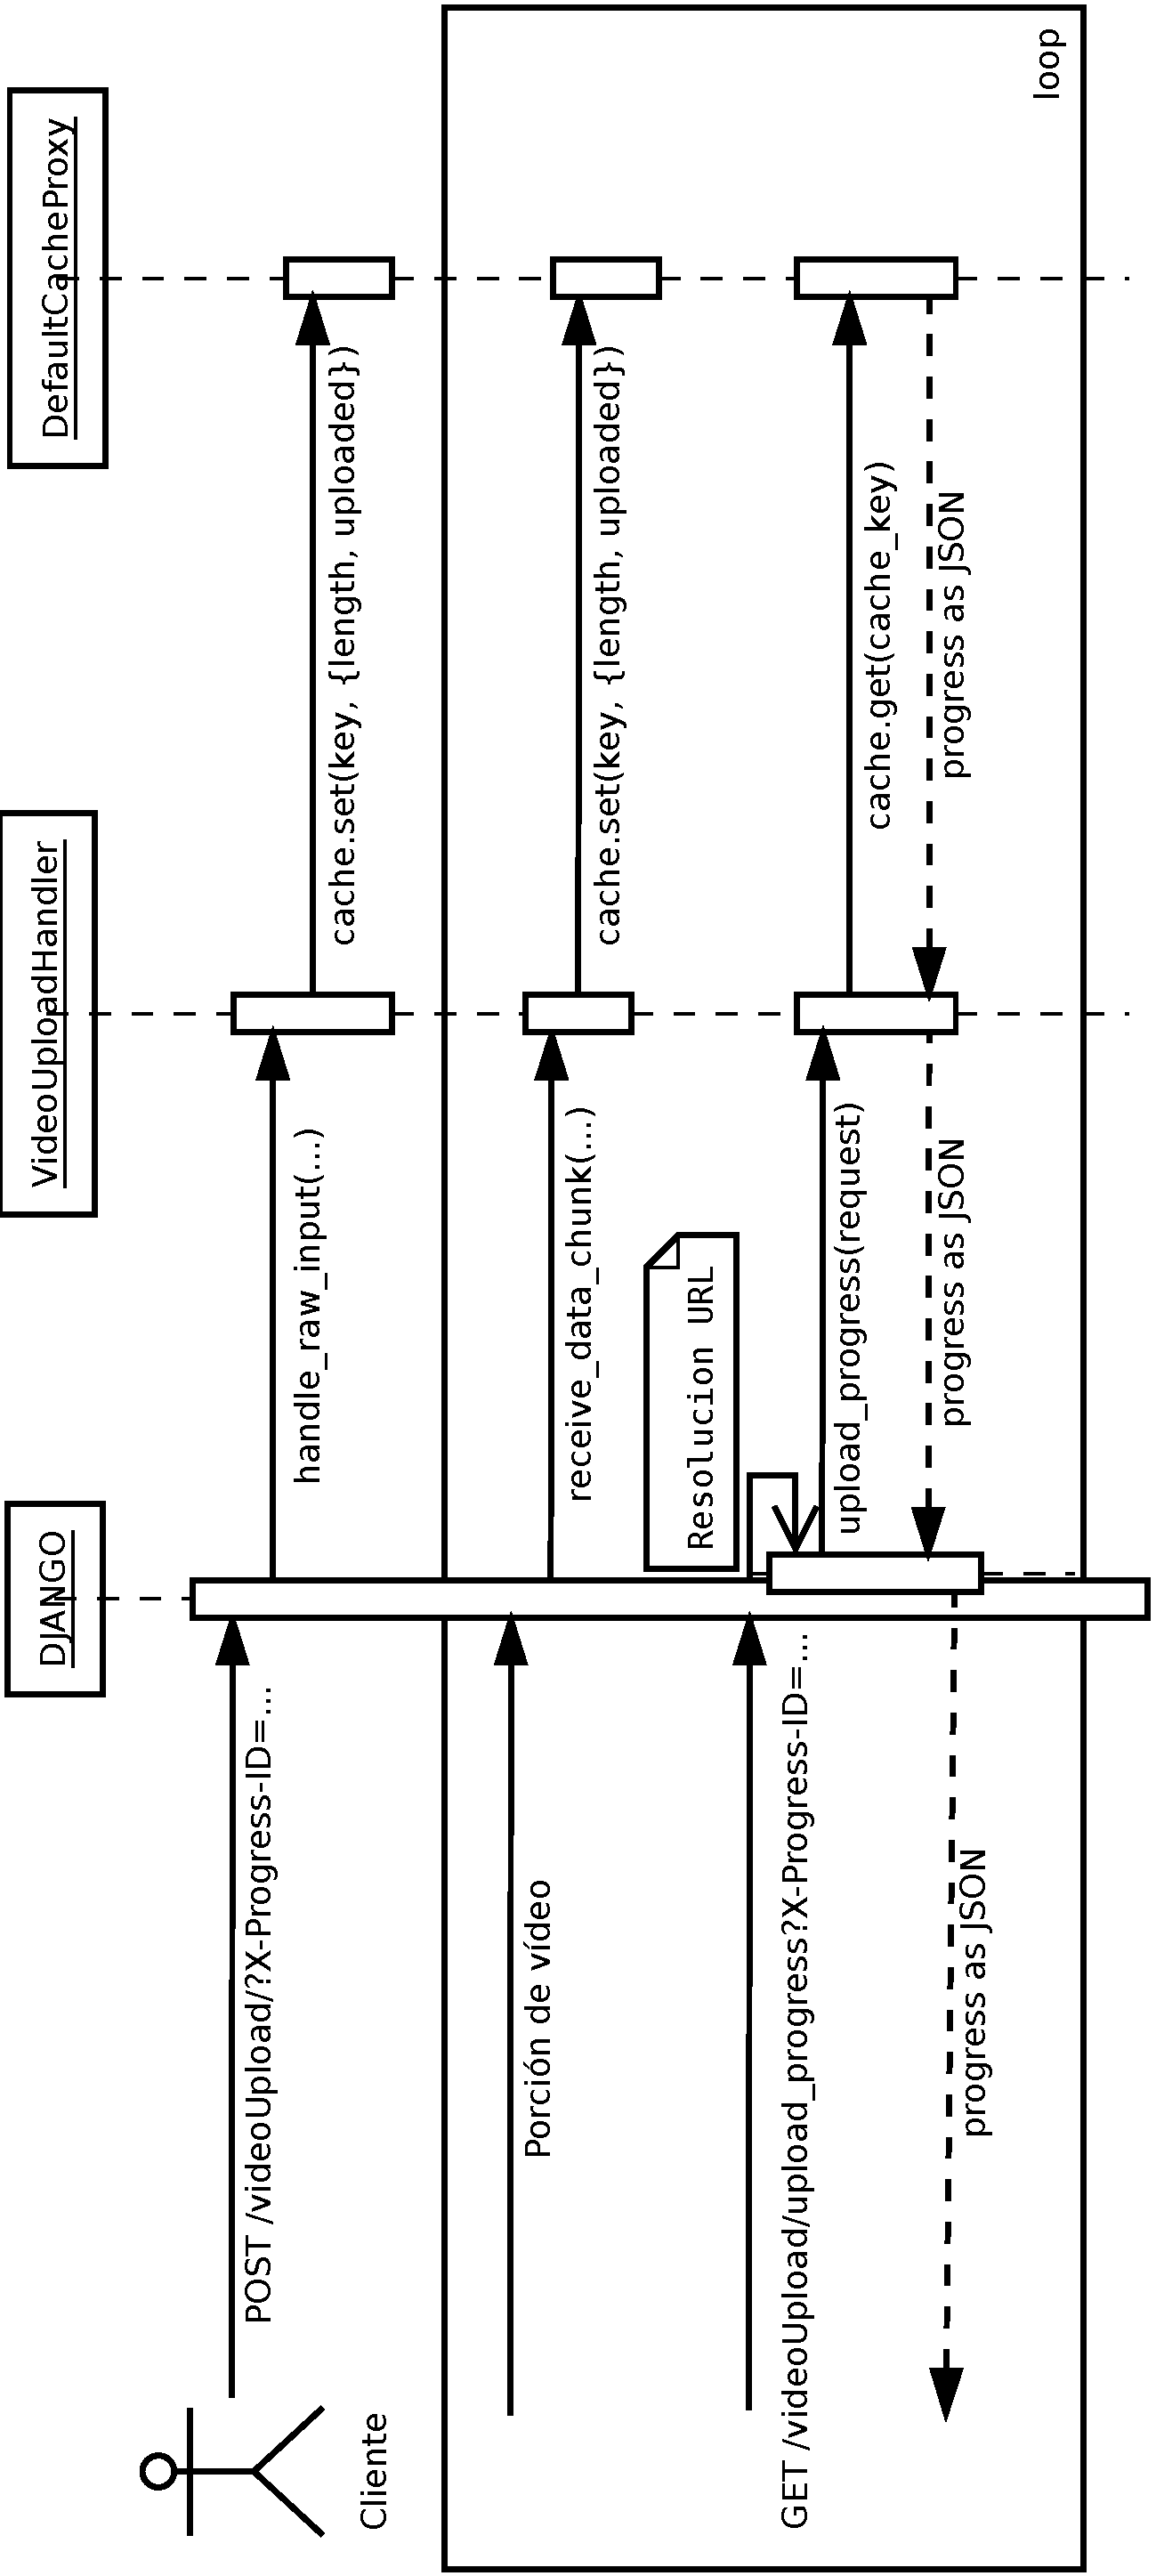
\includegraphics[scale=0.45]{figures/SubidaVideo.pdf}
            \caption{Diagrama de secuencia do proceso seguido cando se fai o Submit do Formulario 
            de creación de vídeos (1)}
        \label{fig:SubidaVideo1}
        \end{center}
        \end{figure}
        
        \begin{figure}[htp]
        \begin{center}
            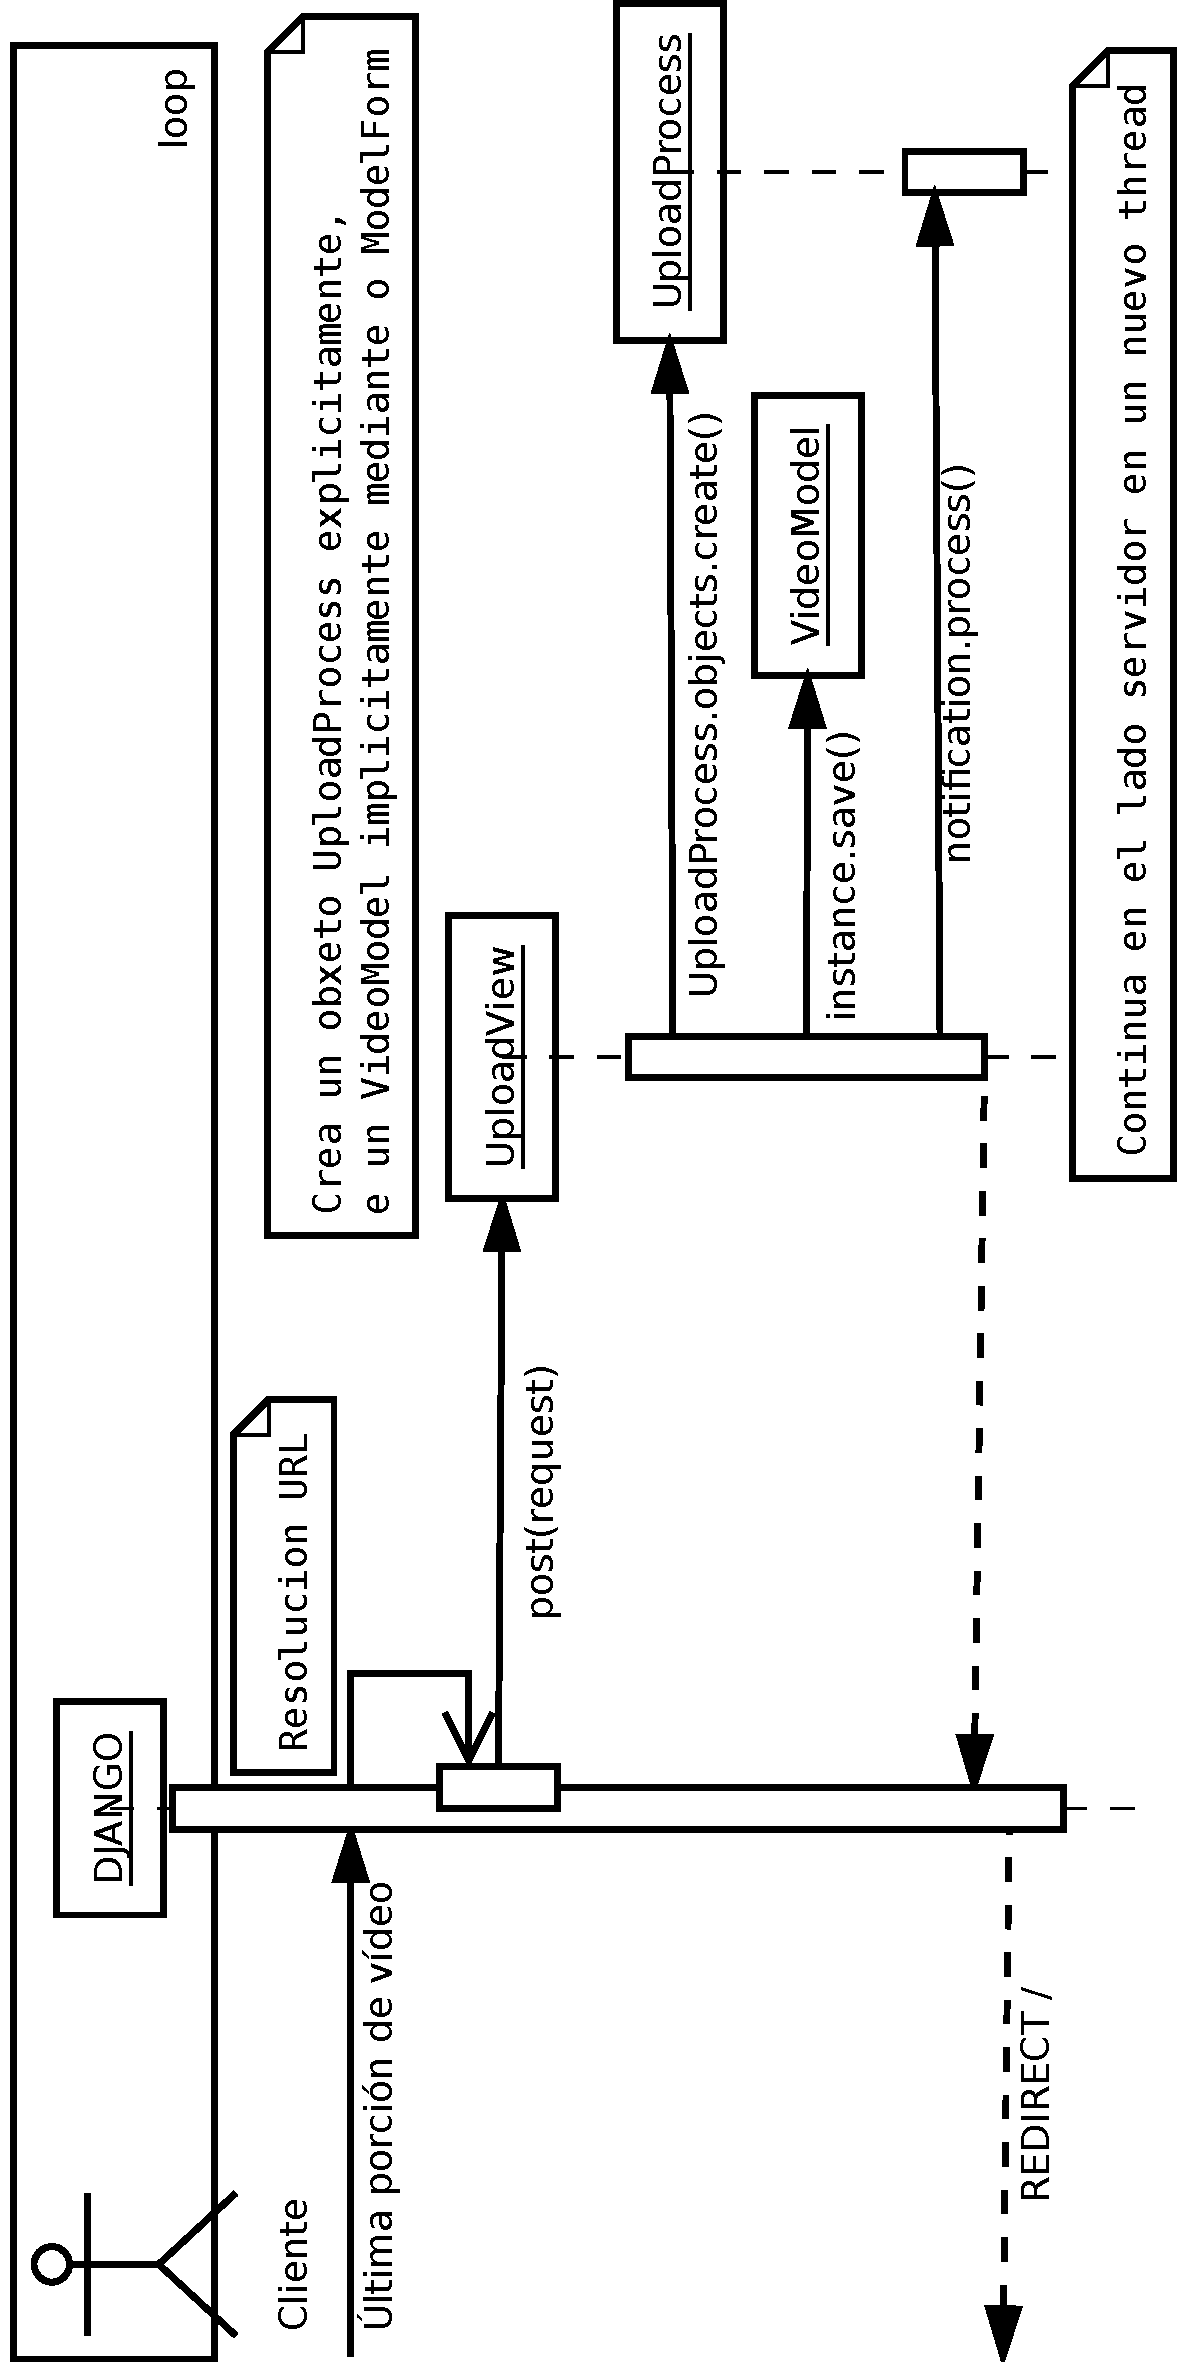
\includegraphics[scale=0.45]{figures/FinSubidaVideo.pdf}
            \caption{Diagrama de secuencia do proceso seguido cando se fai o Submit do Formulario 
            de creación de vídeos (2)}
        \label{fig:FinSubidaVideo2}
        \end{center}
        \end{figure}
                
        
        
        Unha vez subido o vídeo satisfactoriamente agora debese reproducir ese vídeo subido nunha 
        páxina adicada.
            
    \subsection{Reprodución de Vídeo}
        Desexase que a aplicación permita a reprodución dos vídeos contidos, mediante técnicas de
        streaming ou pseudo-streaming. Neste caso empregarase o pseudo-streaming polo sinxela que
        resulta esta implementación empregando as capacidades da etiqueta $<video>$ de HTML5 en conxunto
        con un servidor HTTP como Apache ou o servidor para desenvolvemento de Django.

        \begin{figure}[htp]
        \begin{center}
            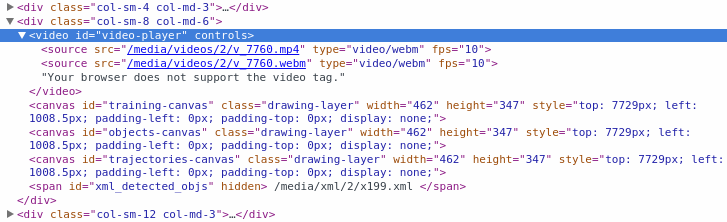
\includegraphics[scale=0.55]{figures/VideoTagHtml5.png}
            \caption{tag en html5, coas súas fontes e coas capas $<canvas>$ asociadas}
        \label{fig:VideoTagHtml5}
        \end{center}
        \end{figure}
        
        na figura \ref{fig:VideoTagHtml5} podemos ver o resultado en HTML5, vense claramente a etiqueta
        $<video>$ coas súas fontes de datos $<source>$, cabe destacar que aquí engadiuse o atributo fps
        (Fotogramas Por Segundo do inglés Frames per second) que non pertence ao estándar definido pola 
        W3C\ref{w3schools-source-tag} mais no caso da nosa aplicación é fundamental para poder coñecer 
        a velocidade á que o navegador vai amosar os fotogramas do vídeo.
        
        Outra cuestión a aclarar é o motivo polo cal non se subministra a fonte de vídeo en formato
        .ogv que a W3C recomenda. A resposta é que o codec theora que ffmpeg inclue soporta 
        decodificación pero NON codificación, polo cal é posible pasar de vídeos en .ogv a outros 
        formatos pero non de outros formatos a .ogv imposibilitando pois que se poida ofrecer o 
        vídeo neste formato mentres o codec de ffmpeg non o permita. Non obstante, isto non supón un 
        problema, xa que como se pode ver na táboa seguinte todos os navegadores permiten a reprodución
        baseándose nestes dous formatos:
        
        \begin{table}[]
            \centering
            \label{supported-video-formats}
            \begin{tabular}{llll}
            \hline
                \multicolumn{1}{c}{\bfseries Navegador} & 
                \multicolumn{1}{c}{\bfseries MP4} & 
                \multicolumn{1}{c}{\bfseries WebM} & 
                \multicolumn{1}{c}{\bfseries Ogg} \\

                \rowcolor[HTML]{EFEFEF} 
                Internet Explorer & SI                                                                                              & NON & NON \\
                Chrome            & SI                                                                                              & SI  & SI  \\
                \rowcolor[HTML]{EFEFEF} 
                Firefox           & \begin{tabular}[c]{@{}l@{}}SI \\ dende Firefox 21 (win)\\ dende Firefox 30 (linux)\end{tabular} & SI  & SI  \\
                Safari            & SI                                                                                              & NON & NON \\
                \rowcolor[HTML]{EFEFEF} 
                Opera             & \begin{tabular}[c]{@{}l@{}}SI\\ dende Opera 25\end{tabular}                                     & SI  & SI 
            \end{tabular}
            \caption{Táboa de formatos de vídeo soportados polos distintos navegadores}
        \end{table}

    
\section{v0.2  Subida e conversión de vídeos }

    Nesta segunda iteración, deséxanse acometer dúas tarefas principais que teñen que ver coa 
    usabilidade da aplicación. Por unha parte crear un listado de vídeos subidos á aplicación para 
    poder acceder a eles de xeito ordenado, e por
    outra parte interesa dar soporte aos procesos de conversión do vídeos a distintos formatos, 
    á análise do vídeo(que se implementará en futuras iteracións) e á extracción de imaxes para 
    empregalas como imaxes representativas do vídeo, dunha forma fluída e estética.
    
    \subsection{Lista de vídeos e Imaxe de Portada}
        
        Co fin de que os usuarios accedan aos distintos vídeos subidos, deseñase unha páxina web que será a
        principal do módulo video\_manager na cal un usuario pode visualizar unha \textbf{ lista paxinada dos
        vídeos} dispoñibles. Esta lista estará ordenada comezando polo vídeo mais recente e rematando
        polo mais antigo, tamén se contempla a posibilidade de poder filtralos por exemplo polo nome.
        
        Para a elaboración de esta páxina empreganse o elementos dos que dispón Django como son a
        clase ListView co seu atributo paginate\_by e o filtrado de resultado co método 
        QuerySet.filter(...), mentres que para o paso das palabras claves polas que buscar un vídeo
        empregase un parámetro de URL chamado 'name'.\\
        
        Outra funcionalidade interesante de cara a amosar unha lista de vídeos é a de poder mostrar unha
        imaxe representativa de cada un deles. Con este fin crease a vista SuccessfulUpload (imaxe
        \ref{fig:SuccessfulUploadScreen}), á que se redirecciona unha vez o vídeo é subido correctamente
        para seleccionar a súa \textbf{imaxe de portada}.
        
        \begin{figure}[htp]
        \begin{center}
            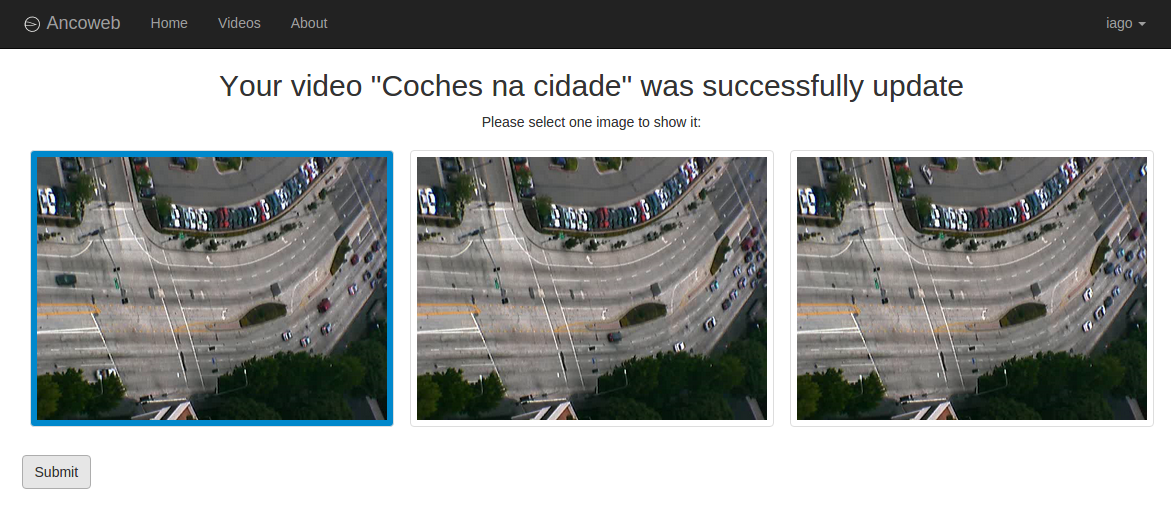
\includegraphics[scale=0.35]{figures/SuccessfulUploadScreen.png}
            \caption{Captura de pantalla da páxina web SuccessfulUpload}
        \label{fig:SuccessfulUploadScreen}
        \end{center}
        \end{figure}
        
        Con este fin extráense mediante ffmpeg unha serie de fotogramas do vídeo, que se gardan nun
        directorio temporal para que unha vez o vídeo estea subido e analizado, as imaxes se integren 
        como parte dun formulario na páxina SuccessfulUpload. Mediante este formulario, xerado co plugin
        image-picker\cite{ImagePickerPage}, o usuario poderá escoller o fotograma que lle pareza mais
        representativo do vídeo e unha vez que pulse no botón de ''Submit'' este fotograma gardarase
        como parte do Modelo de Django VideoModel, quedando pois accesible para que a lista de vídeos 
        poida amosalo.
        
    \subsection{Sistema de Notificacións}
    
        Cando deseñamos unha aplicación web é de capital importancia que o usuario este informado de que está
        a acontecer na aplicación para que non sinta que está perdido, ou que a aplicación non responde. Tendo
        isto en conta, e sabendo que tanto o proceso de análise(que inda non está implementado)
        coma o de conversión do vídeo a outros 
        formatos poden requirir dun tempo prolongado, prantexase un problema: como manter ao usuario informado
        destes longos procesos e evitar a sensación de bloqueo?\\
        
        A solución deseñada é un sistema de notificacións que permite ao usuario rexistrado navegar libremente
        pola aplicación mentres o vídeo se está a analizar, mostrando en todo momento unha barra de progreso
        para o proceso que se está a seguir nestes intres como se pode observar na imaxe 
        \ref{fig:Notificacions}.
        
        \begin{figure}[htp]
        \begin{center}
            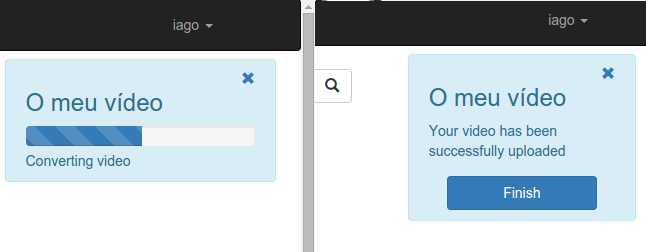
\includegraphics[scale=0.5]{figures/Notificacions.png}
            \caption{Capturas de pantalla do sistema de Notificacións}
        \label{fig:Notificacions}
        \end{center}
        \end{figure}
        
        Para albergar tanto o sistema de notificacións como os procesos que engloba, creouse o módulo de 
        Django video\_upload composto polas clases que se poden observar no diagrama \ref{fig:ClassDiagram}.

        \begin{figure}[htp]
        \begin{center}
            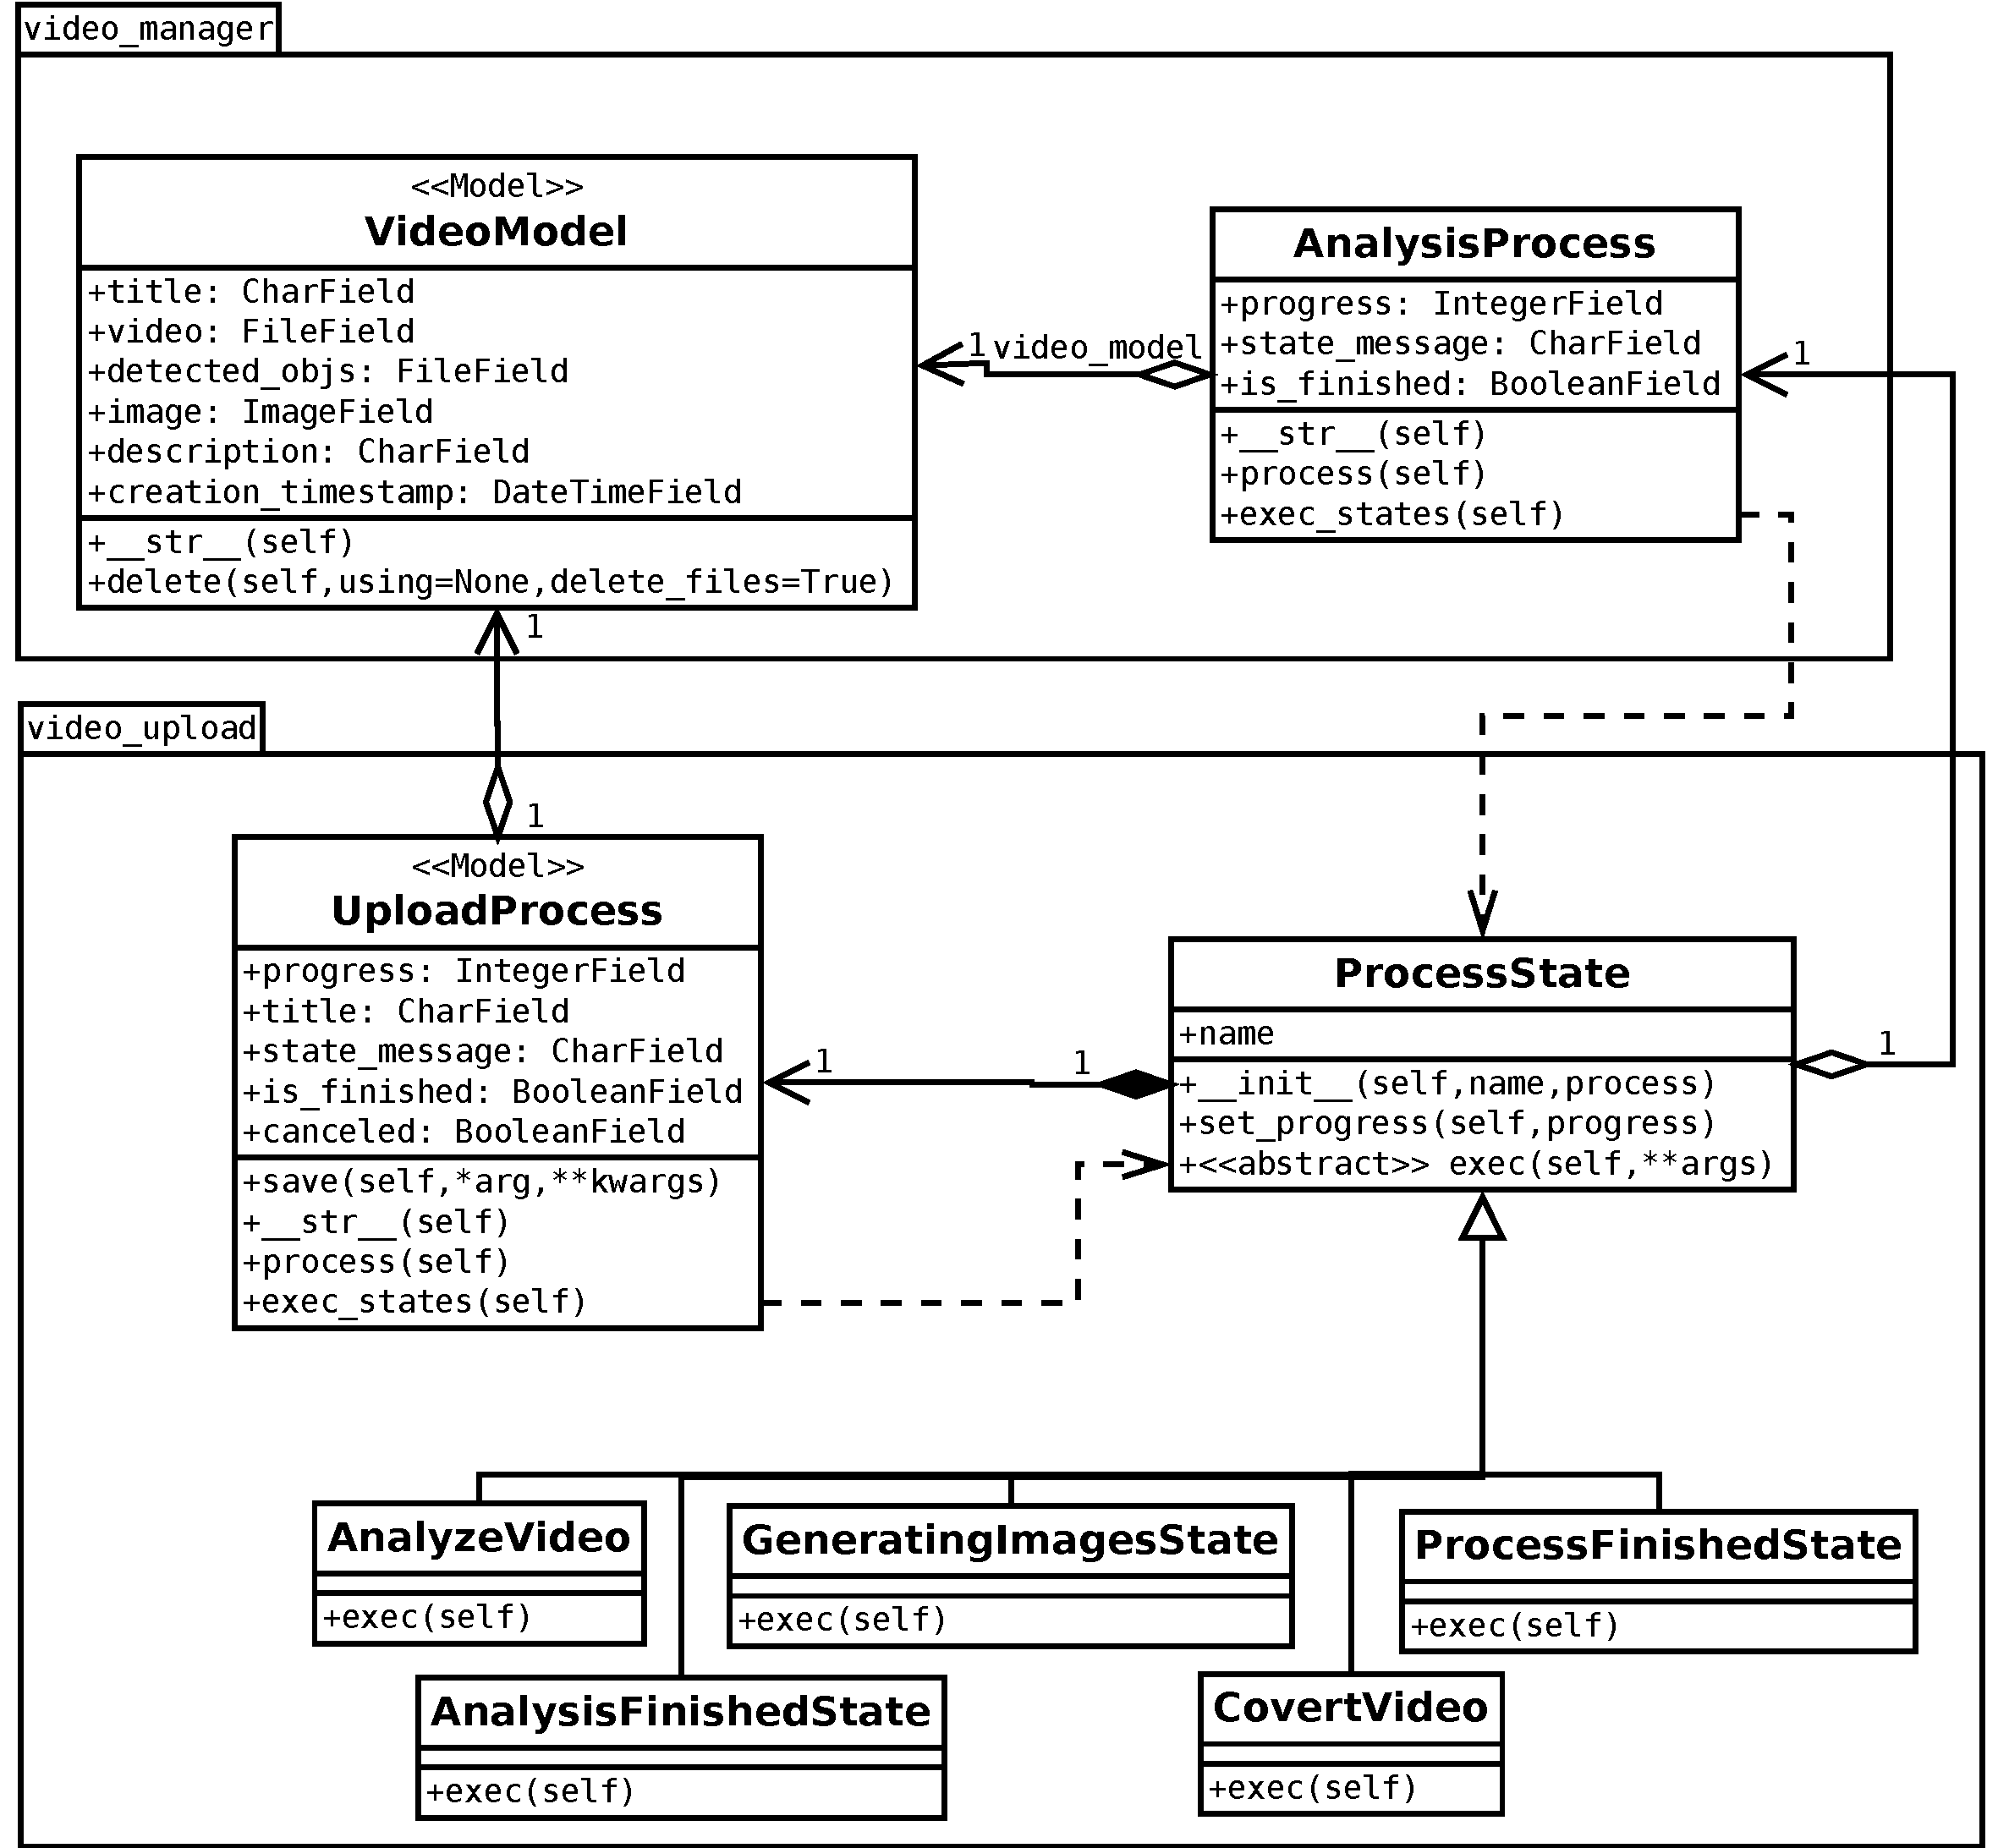
\includegraphics[scale=0.4]{figures/ClassDiagram.pdf}
            \caption{Diagrama de Clases do sistema de subida}
        \label{fig:ClassDiagram}
        \end{center}
        \end{figure}
        
        UploadProcess representa o proceso de subida, análise, conversión e extracción de imaxes
        a partir de un vídeo. Mentres que AnalysisProcess representa o proceso que se segue no 
        caso de que un vídeo xa subido á plataforma sexa analizado de novo. Os distintos estados
        nos que pode estar un proceso modelanse mediante a clase abstracta ProcessState, que nas
        súas implementacións define tanto o traballo a realizar neste estado coma a mensaxe que 
        se amosará ao usuario cando este se execute.\\
        
        Dado que é o ProcessState que executará a tarefa, tamén será o encargado de actualizar
        a través do método set\_progress(self, progress) o progreso do proceso asociado (
        UploadProcess ou AnalysisProcess).\\
        
        É importante destacar que as figuras etiquetadas co estereotipo $<<Model>>$ son modelos 
        de BD manexados por Django. Nótese tamén que pese a que UploadProcess e AnalysisProcess
        comparten a meirande parte do seu código, non foron refactorizados nunha clase abstracta,
        dadas as complicacións de base de datos que isto carrexa. En lugar diso empregase o 
        tipado dinámico de Python para pasar os obxectos tanto de UploadProcess como de 
        AnalysisProcess á clase ProcessState, que ao invocar só os métodos comúns non é capaz de 
        percibir a diferenza entre ambas. O seu funcionamento mostrase no gráfico
        \ref{fig:AnaliseVideoWeb}.
        
        \begin{figure}[htp]
        \begin{center}
            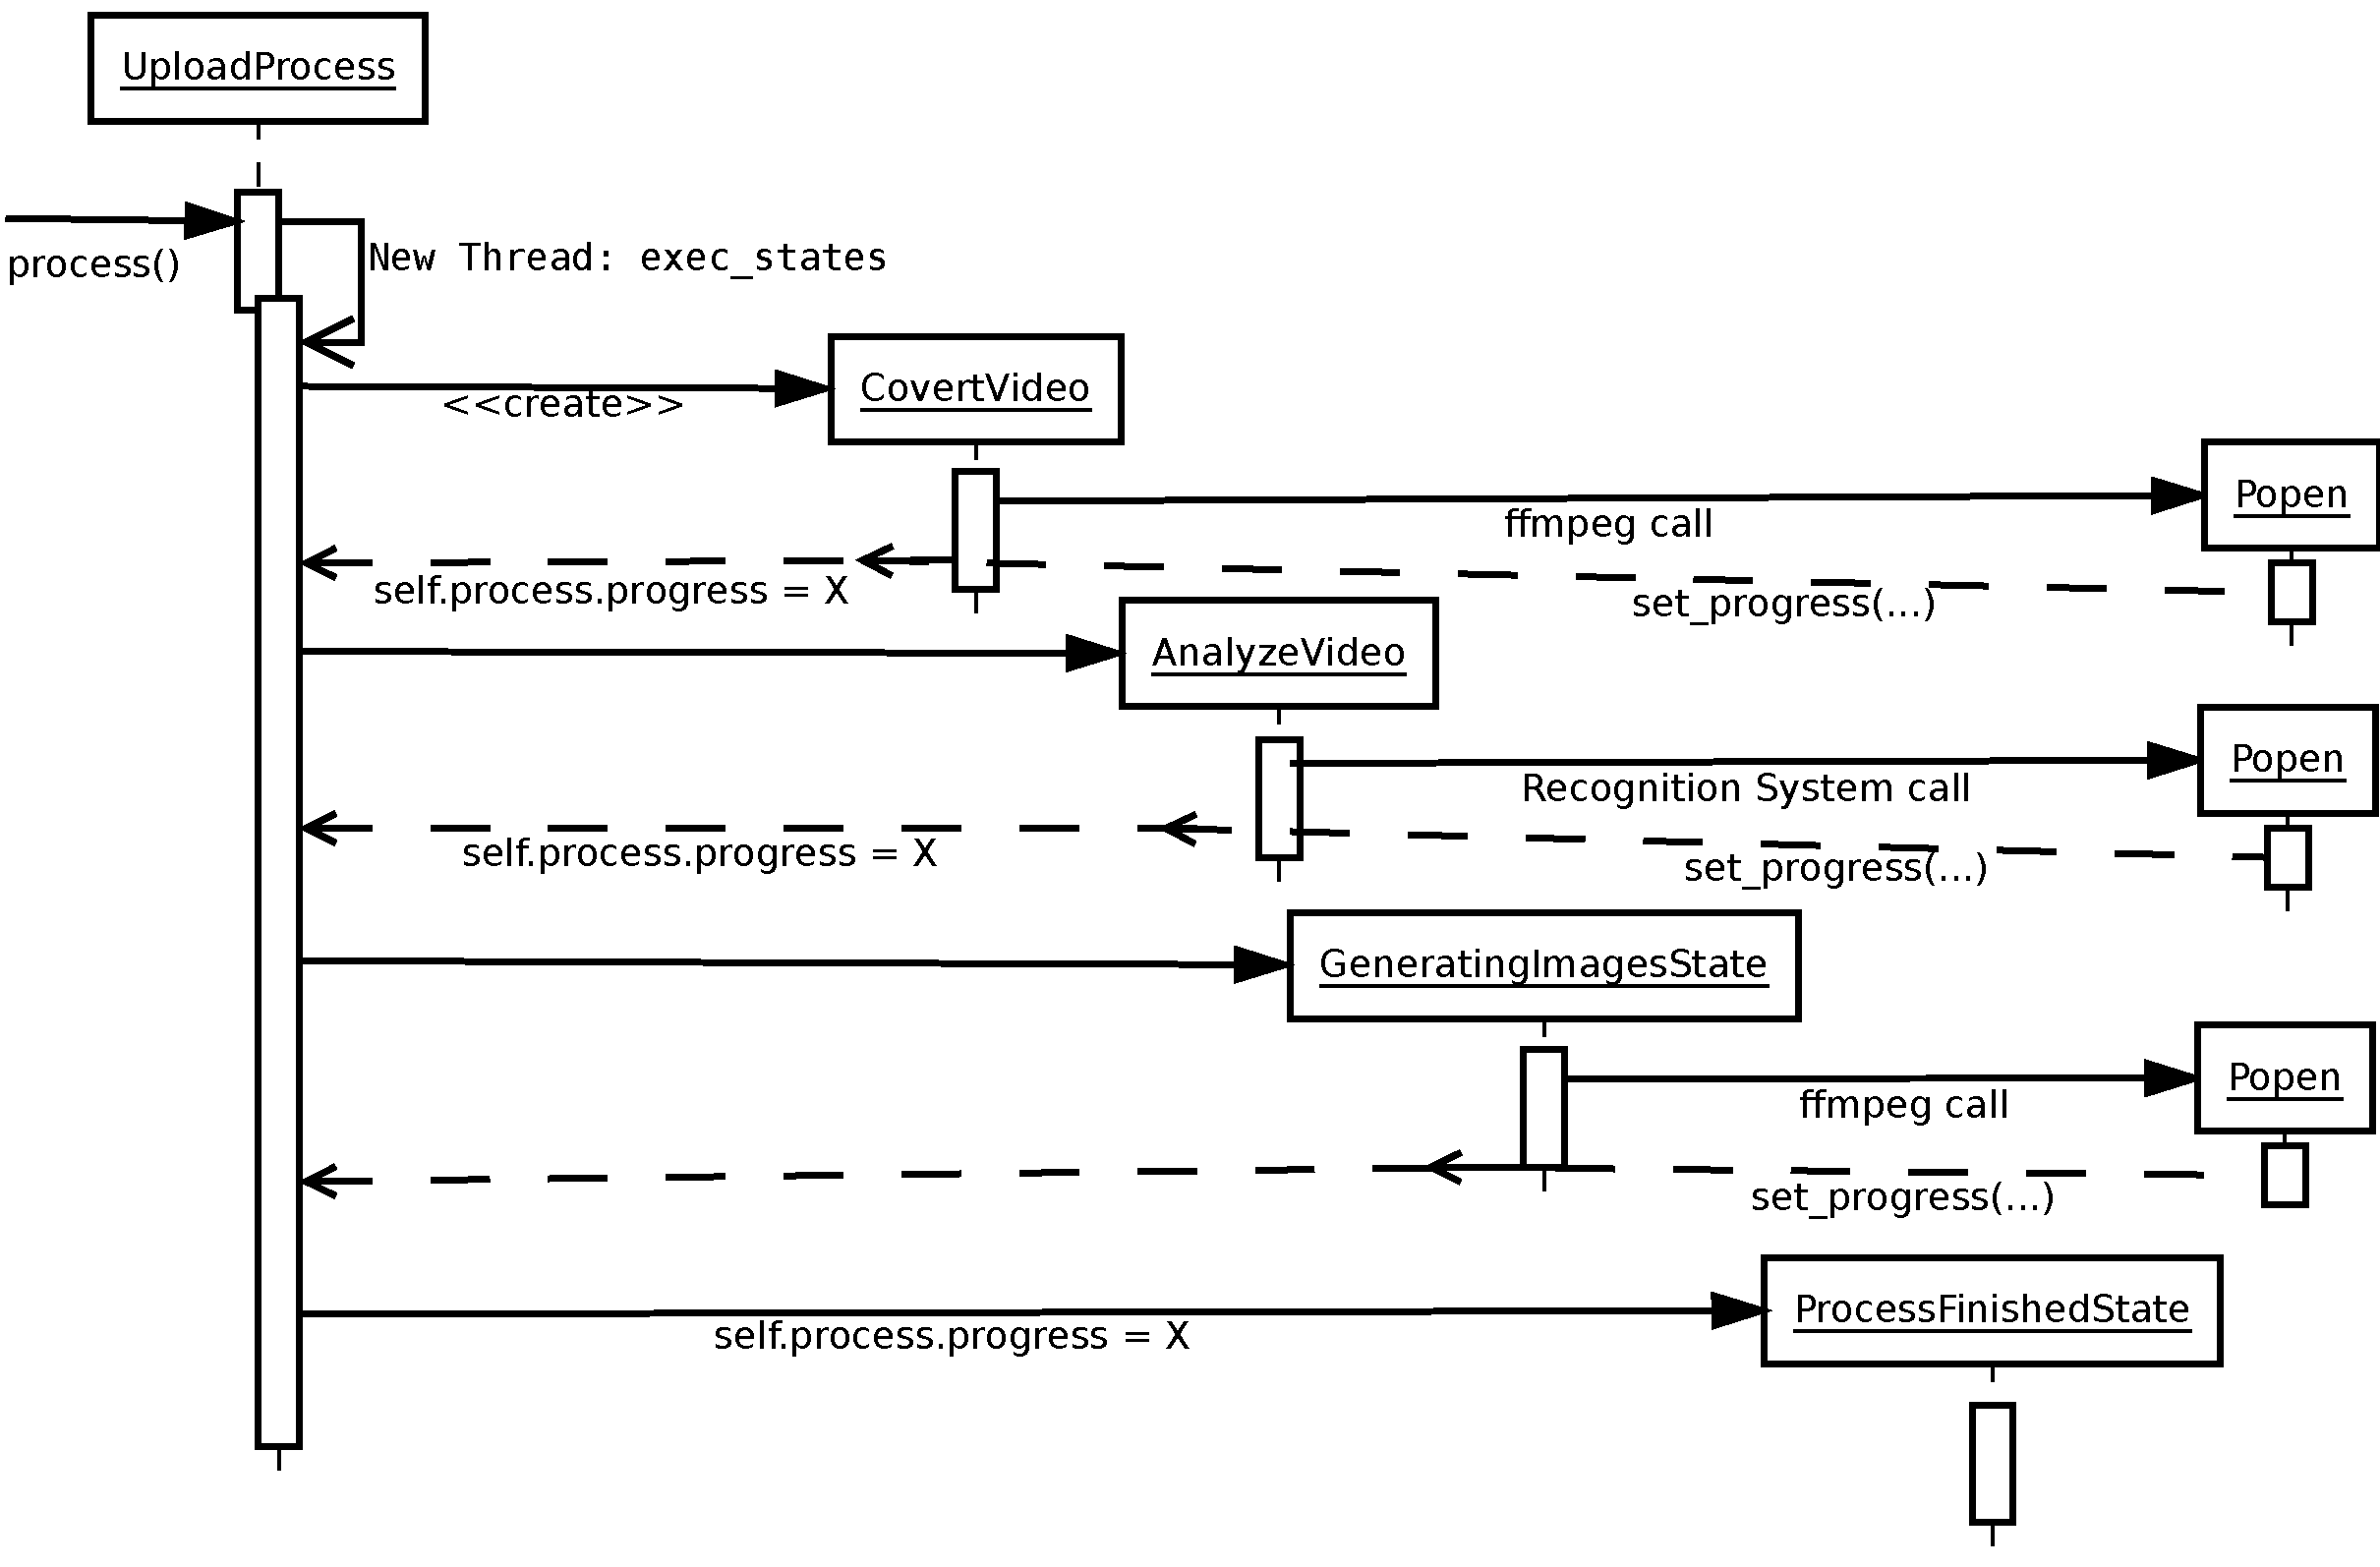
\includegraphics[scale=0.35]{figures/AnaliseVideoWeb.pdf}
            \caption{Diagrama de secuencia da análise do vídeo na capa web}
        \label{fig:AnaliseVideoWeb}
        \end{center}
        \end{figure}
    
\section{v0.3 Xerar e mostrar deteccións básicas}

    En esta iteración tratouse tanto a análise do vídeo creando o sistema de recoñecemento, como 
    o xeito de amosar os resultados destes na capa web, todo elo deseñado de xeito flexible e 
    modulado como se explica a continuación.
    
    \subsection{Análise de Vídeo}
        Para a análise de vídeo será preciso definir unha interface de liña de comandos mediante
        a cal a aplicación web chamará ao Sistema de Recoñecemento, indicándolle aqueles parámetros
        que sexan precisos\ref{fig:InterfazLineaComandos}.

        \subsubsection{Interface de Liña de Comandos}
        A aplicación web indicaralle a este sistema o vídeo que debe empregar como entrada para o 
        recoñecemento e o ficheiro de saía onde ten que escribir os datos da análise. A maiores, pódeselle
        indicar con que frecuencia se desexa que o Subsistema Behaviour System, encargado da análise de
        alto nivel, entre en funcionamento. Po último a opción --standar fai que se mostre o resultado da
        detección de obxectos por liña de comandos, esta saída é empregada pola capa web para calcular o
        progreso do proceso de análise.\\
        
        Estas opcións tamén se poden visualizar mediante o comando --help:\\ 
        \begin{verbatim}
    iago@UbuIago:~/TFG/src/RecognitionSystem$ ./recognitionsystem --help
    Usage:   recognitionsystem
    option:  
    -i          --input      <path/to/outputFile.xml> Set the input file.
    -o          --output     <path/to/outputFile.xml> Set the output file.
    -f [value]  --frequency  Determines after how many frames the Behaviour 
                            System checks the minimal path
    --standar                Print the xml into the standar output.
    --verbose
        \end{verbatim}
        
        \begin{figure}[htp]
        \begin{center}
            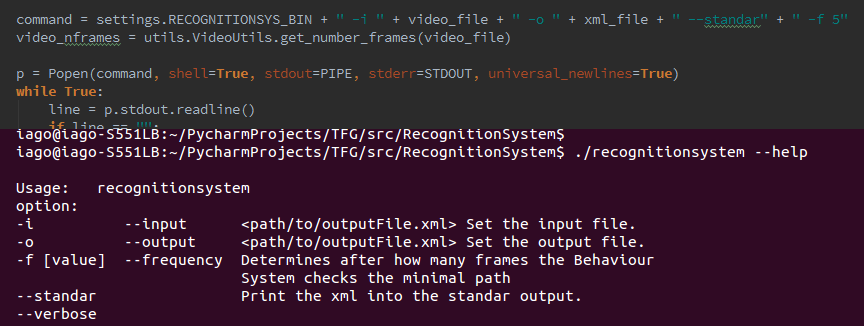
\includegraphics[scale=0.45]{figures/InterfazLineaComandos.png}
            \caption{Interfaze de liña de comandos do Sistema de recoñecemento}
        \label{fig:InterfazLineaComandos}
        \end{center}
        \end{figure}
        
        \subsubsection{Ficheiro XML}
            Como resultado desta chamada, o sistema de recoñecemento debe crear no ficheiro indicado 
            para a saída, un XML co formato que se define no esquema .dtd situado no directorio
            
            \begin{verbatim}
            src/static/detections\_schema.dtd
            \end{verbatim}       

            Neste ficheiro podemos ver a definición dos seguintes elementos:
            \begin{itemize}
            \item{{\textbf{$<objects>$\\}}}
                Contén para cada un dos fotogramas $<frame>$ a lista de obxectos detectados segundo
                o explicado no apartado \ref{cap:DeteccionObxetos}, indicando para cada un deles a
                distancia á parte esquerda, e superior da escena (xc, yc) e o alto e ancho do obxecto
                detectado (h, w).
            \item{{\textbf{$<trajectories>$\\}}}
                Este outro elemento garda para cada un dos obxectos detectados a traxectoria que 
                seguiu ao longo do vídeo, esta traxectoria estará composta de unha serie de puntos
                $<point>$, para cada un dos cales, a parte das súas coordenadas e o número de 
                frame, indicase un grao de anormalidade entre 1 e 0 que indica como de anómala é 
                a conduta dese obxecto no momento no que se atopa sobre ese punto.
            \end{itemize}
            
            Para xerar este ficheiro XML foi preciso desenvolver unha serie de funcionalidades en C++,
            que están contidas no paquete XmlRecognition.
        
        \subsubsection{Paquete XmlRecognition}
            Inicialmente o proxecto conta cun código escrito en C++ e apoiado en OpenCV que está distribuído en
            dúas librerías EllipseLib e BehaviorLib. A primeira delas encargada da detección de obxetos, e a segunda
            encargada de analizalo comportamento a alto nivel a partir dos resultados que proporciona a primeira.\\
            
            Para a construción do Sistema de recoñecemento integraranse estas dúas librerías como módulos, e 
            crearase un terceiro módulo C++ chamado XmlRecognition (figura \ref{fig:PaqXmlRecognition}).
            Este novo módulo será o responsable de definir e implementar a interface de liña de 
            comandos, xestionar a comunicación entre as dúas librerías e gardar o resultado da análise
            en formato XML.
            
            \begin{figure}[htp]
            \begin{center}
                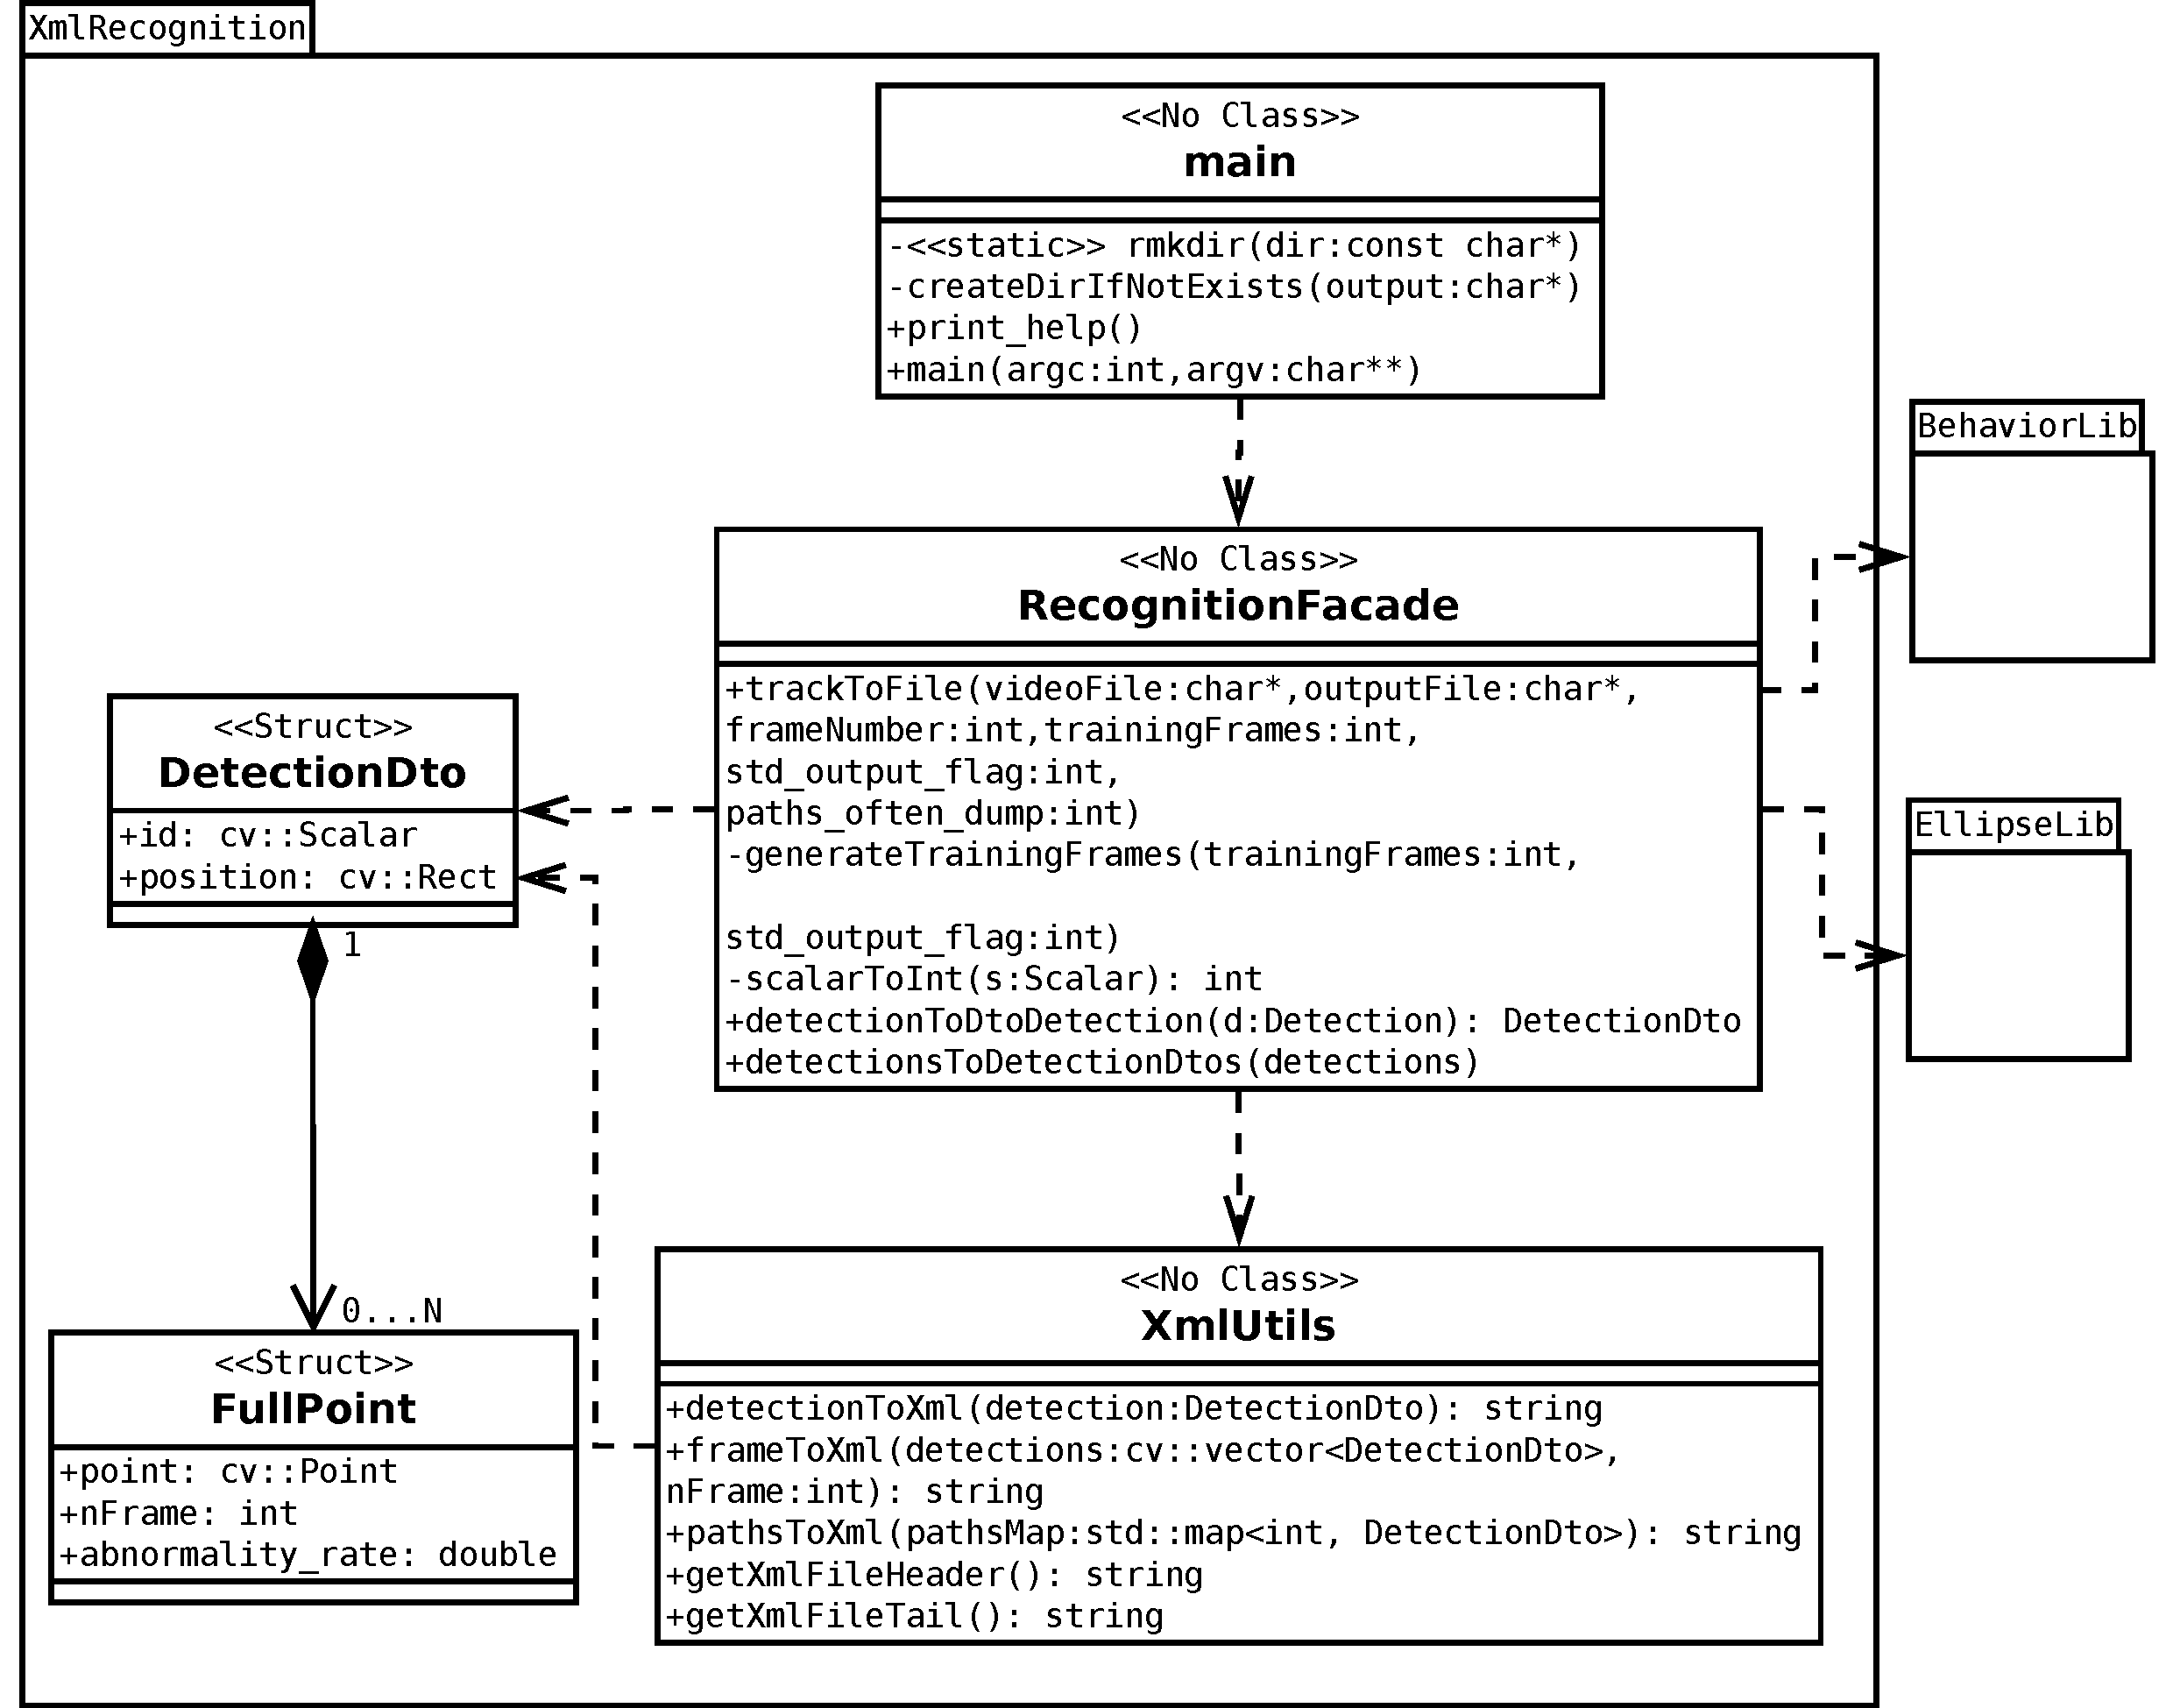
\includegraphics[scale=0.4]{figures/PaqXmlRecognition.pdf}
                \caption{Diagrama de clases do paquete XmlRecognition}
            \label{fig:PaqXmlRecognition}
            \end{center}
            \end{figure}
            
            Para elo, crease un ficheiro principal chamado \textbf{main.cpp} que describe a interface de liña de comandos
            independente da librería que se emprega para as deteccións, un ficheiro \textbf{XmlUtils} que contén as
            funcionalidades para a escritura do XML en base a unha detección simplificada: DetectionDto 
            (Data Transfer Object), e por último un ficheiro \textbf{RecognitionFacade} que variará en 
            caso de cambiar as librarías, transformando o resultado destas en DetectionDto's para logo
            poder escribilo coas funcionalidades de XmlUtils.
            
            Para maximizar o rendemento evitase crear clases innecesarias: para o caso da DetectionDto é dabondo
            cunha estrutura, e no caso de XmlUtils y RecognitionFacade, ao non ter estado chega con ficheiros
            que definen funcións.
            
            Coa elaboración deste paquete queda listo o sistema de recoñecemento, agora solo resta que a capa web
            sexa capaz de chamar ao sistema e mostrar as análises en XML sobre o vídeo. Será o que abordaremos
            no seguinte apartado.

    \subsection{Mostrar Deteccións}
        
        Unha vez que o vídeo xa está subido e correctamente analizado, o que resta é comezar a construír
        na capa web as vistas que mostren sobre o elemento $<video>$ de HTML5 as distintas capas de 
        análise obtidas a partires do ficheiro XML, así como unha serie de paneis que permitan 
        configurar estas vistas.
        
        Todo este traballo realizase na vista DetailsView do módulo video\_manager e principalmente 
        consiste nun ficheiro HTML que contén as referencias a:
        \begin{itemize}
        \item O vídeo a mostrar
        \item O ficheiro XML que contén a análise realizada polo sistema de recoñecemento.
        \item Os ficheiros de estilo.
        \item Os distintos ficheiros de código javascript involucrados.
        \end{itemize}
        
        Para amosar a análise do ficheiro XML sobre o vídeo a estratexia será a de a de superpoñer 
        distintos elementos $<canvas>$ sobre o elemento vídeo $<video>$ como se pode ver na figura 
        \ref{fig:VideoTagHtml5}. Para axustar todas estas capas etiquetadas como class=``drawing-layer''
        sobre o vídeo crease a función adjustCanvasExtended do ficheiro video-player.js, esta función 
        chamase cando o vídeo se carga na páxina, en caso de que o tamaño do vídeo cambie ou cando se 
        entra e sae do modo pantalla completa, axustando de novo o tamaño de todas estas capas ao actual
        tamaño do vídeo.
        
        Unha vez axustados os elementos $<canvas>$ nos que se desexa amosar a información, tense que 
        extraer esta do ficheiro XML. O XML cargase mediante AJAX, cunha chamada de jQuery \$.get(...) 
        ao dirección do servidor que indica a etiqueta oculta con id xml\_detected\_objs, unha vez cargado
        este arquivo iniciase a carga inicial do sistema.
        
        Esta carga inicial consiste na creación dun obxecto VideoDetections creado a partir do XML, e
        que conterá a lista de deteccións así como unha referencia ao elemento $<video>$. Este elemento
        VideoDetections, é o suxeito de un patrón Observador no cal un suxeito ou obxecto central
        notifica ao seus observadores (Observers) os cambios no seu estado. Neste caso, os observadores
        serán os encargados de actualizar cada un dos elementos da páxina, incluídas as capas $<canvas>$,
        dos cambios no suxeito VideoDetections, estes cambios poden ser por exemplo o avance na 
        reprodución do vídeo, un cambio de preferencias no panel de control... Deste xeito unificase a 
        xestión das deteccións que só se manexa no elemento VideoDetections e faise moito mais sinxelo 
        engadir ou eliminar algunha capa de información xa que basta con engadir ou eliminar o 
        observador que a manexa.
        
        Nótese que a maiores do propio patrón observador, tamén se engaden os métodos enable e disable á
        clase DetectionsObserver, isto faise para que no caso de que algún observador non se atope 
        activo nun momento determinado non reciba as notificacións de actualización. O motivo deste
        cambio é o incremento de eficiencia que produce, moi importante dado que o proceso de actualización
        do Suxeito e todo-los seus observadores tense que executar entre 10 e 30 veces por segundo, todo
        isto pódese ver reflexado no diagrama da figura \ref{fig:observerPattern}.
        
        \begin{figure}[htp]
        \begin{center}
            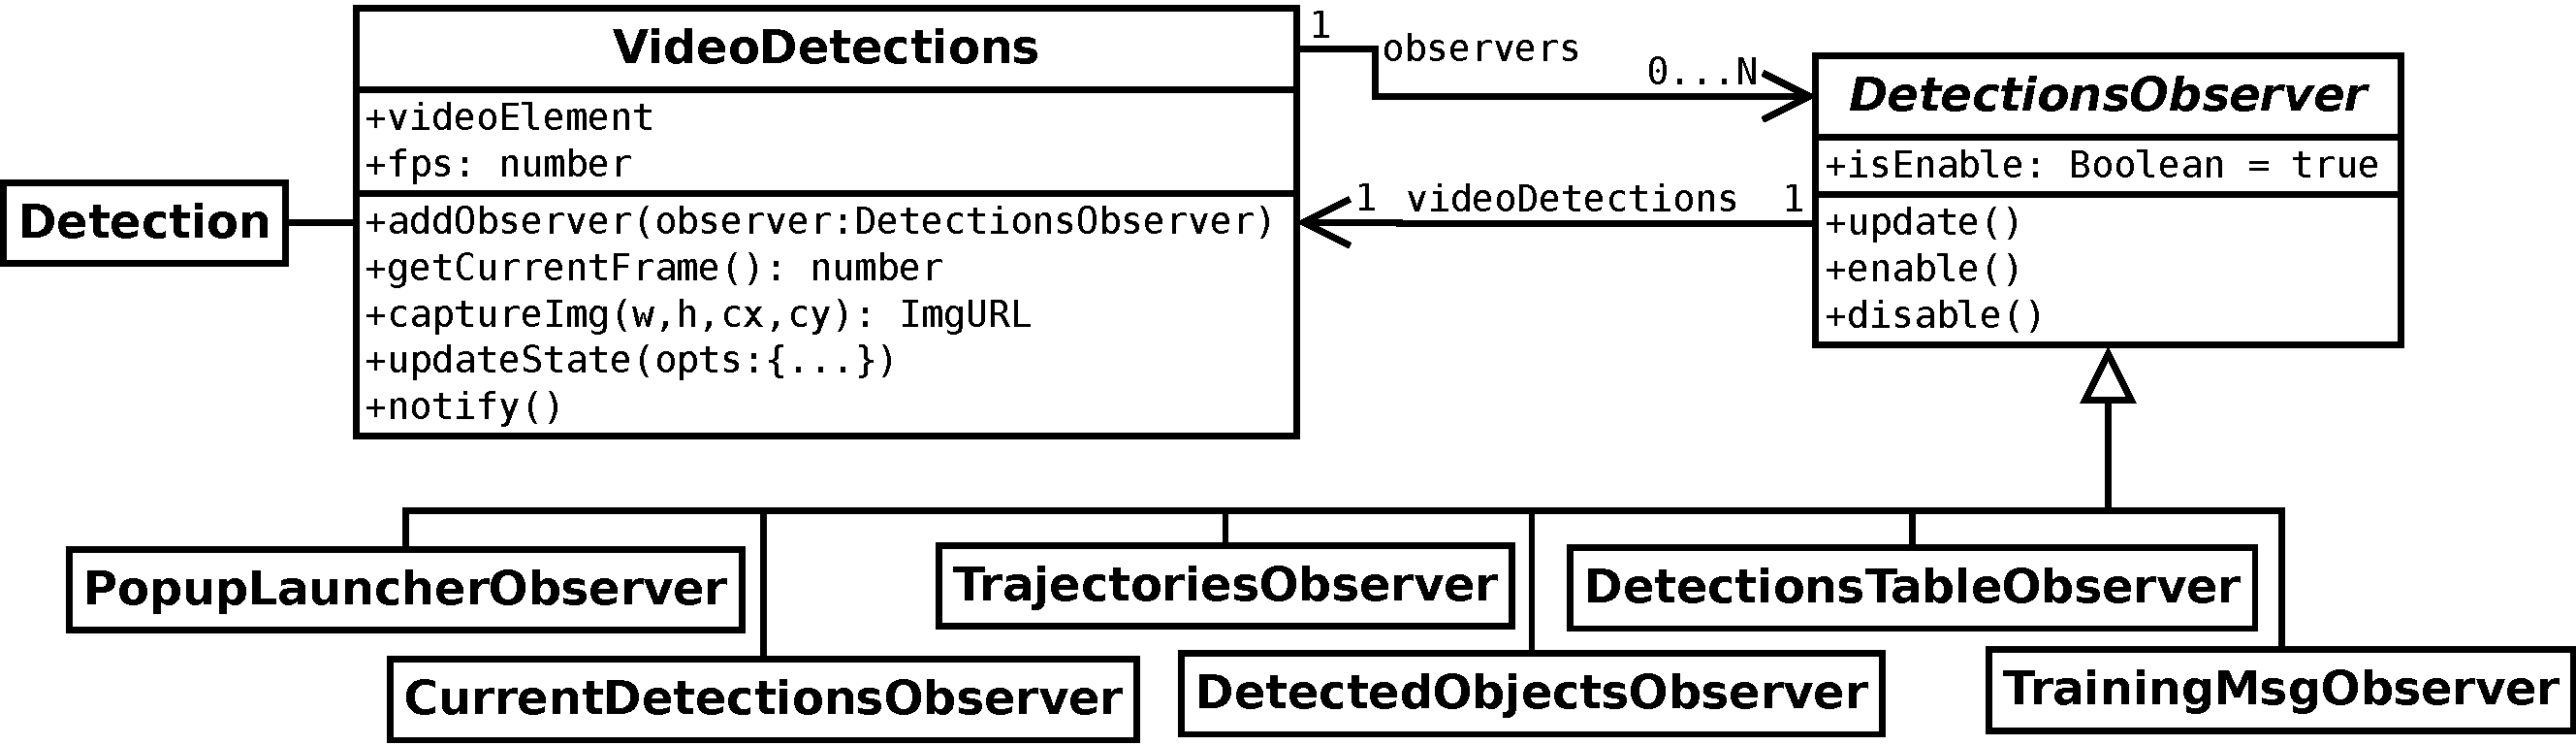
\includegraphics[scale=0.35]{figures/observerPattern.pdf}
            \caption{Diagrama de clases simplificado do patrón observador na capa web}
        \label{fig:observerPattern}
        \end{center}
        \end{figure}
        
        Agora que se coñece o xeito no que as deteccións pasan de un formato xml a un modelo obxectual 
        no cal poden ser consultadas con maior eficiencia veremos como actualizar o estado dos elementos
        $<canvas>$ cada vez que se mostra un novo fotograma ou se modifica algunha opción dos paneis da
        páxina.
        
        Nun comezo, pensouse en asociar a actualización de estado ao evento timeupdate do elemento 
        $<video>$, que segundo a súa definición lanzase cando a posición do vídeo varía. Por desgraza, 
        e como reflexa a reflexión que podemos atopar no libro \cite[Capítulo 6.1]{video-con-html5}
        este evento é lento de mais para o seu emprego, polo que o que se fará será
        crear un bucle que se execute cando o vídeo se estea a reproducir. Para tentar que o bucle se 
        execute unha soa vez en cada un dos fotogramas empregase a función setTimeout que fará que o 
        código agarde unha cantidade de tempo antes de volver a executarse. Esta cantidade de tempo 
        calculase en base ás dez execucións anteriores e ao número de fotogramas por segundo como se
        pode ver na seguinte formula:
        
        \vspace{1cm}
        \begingroup\makeatletter\def\f@size{16}\check@mathfonts
            $ t_n = \frac{1000}{videoDetections.fps} - \frac{\sum_{i=0}^{10} lastUpdateTimes[i]}{10}$
        \endgroup
        \vspace{1cm}
        
        O número de fotogramas por segundo para esa fonte ao que se accede mediante o obxecto 
        videoDetections obtense grazas a que o servidor o inclúe no HTML mediante o atributo fps en 
        cada elemento $<source>$ do elemento $<video>$ como se ve na figura \ref{fig:VideoTagHtml5}.
        Á súa vez o servidor obtén estes datos para as distintas fontes de vídeo dunha chamada ao
        método VideoUtils.get\_fps que chama ao ffmpeg como se ve no diagrama de secuencia 
        \ref{fig:GenerateFpsDjango}.
        
        \begin{figure}[htp]
        \begin{center}
            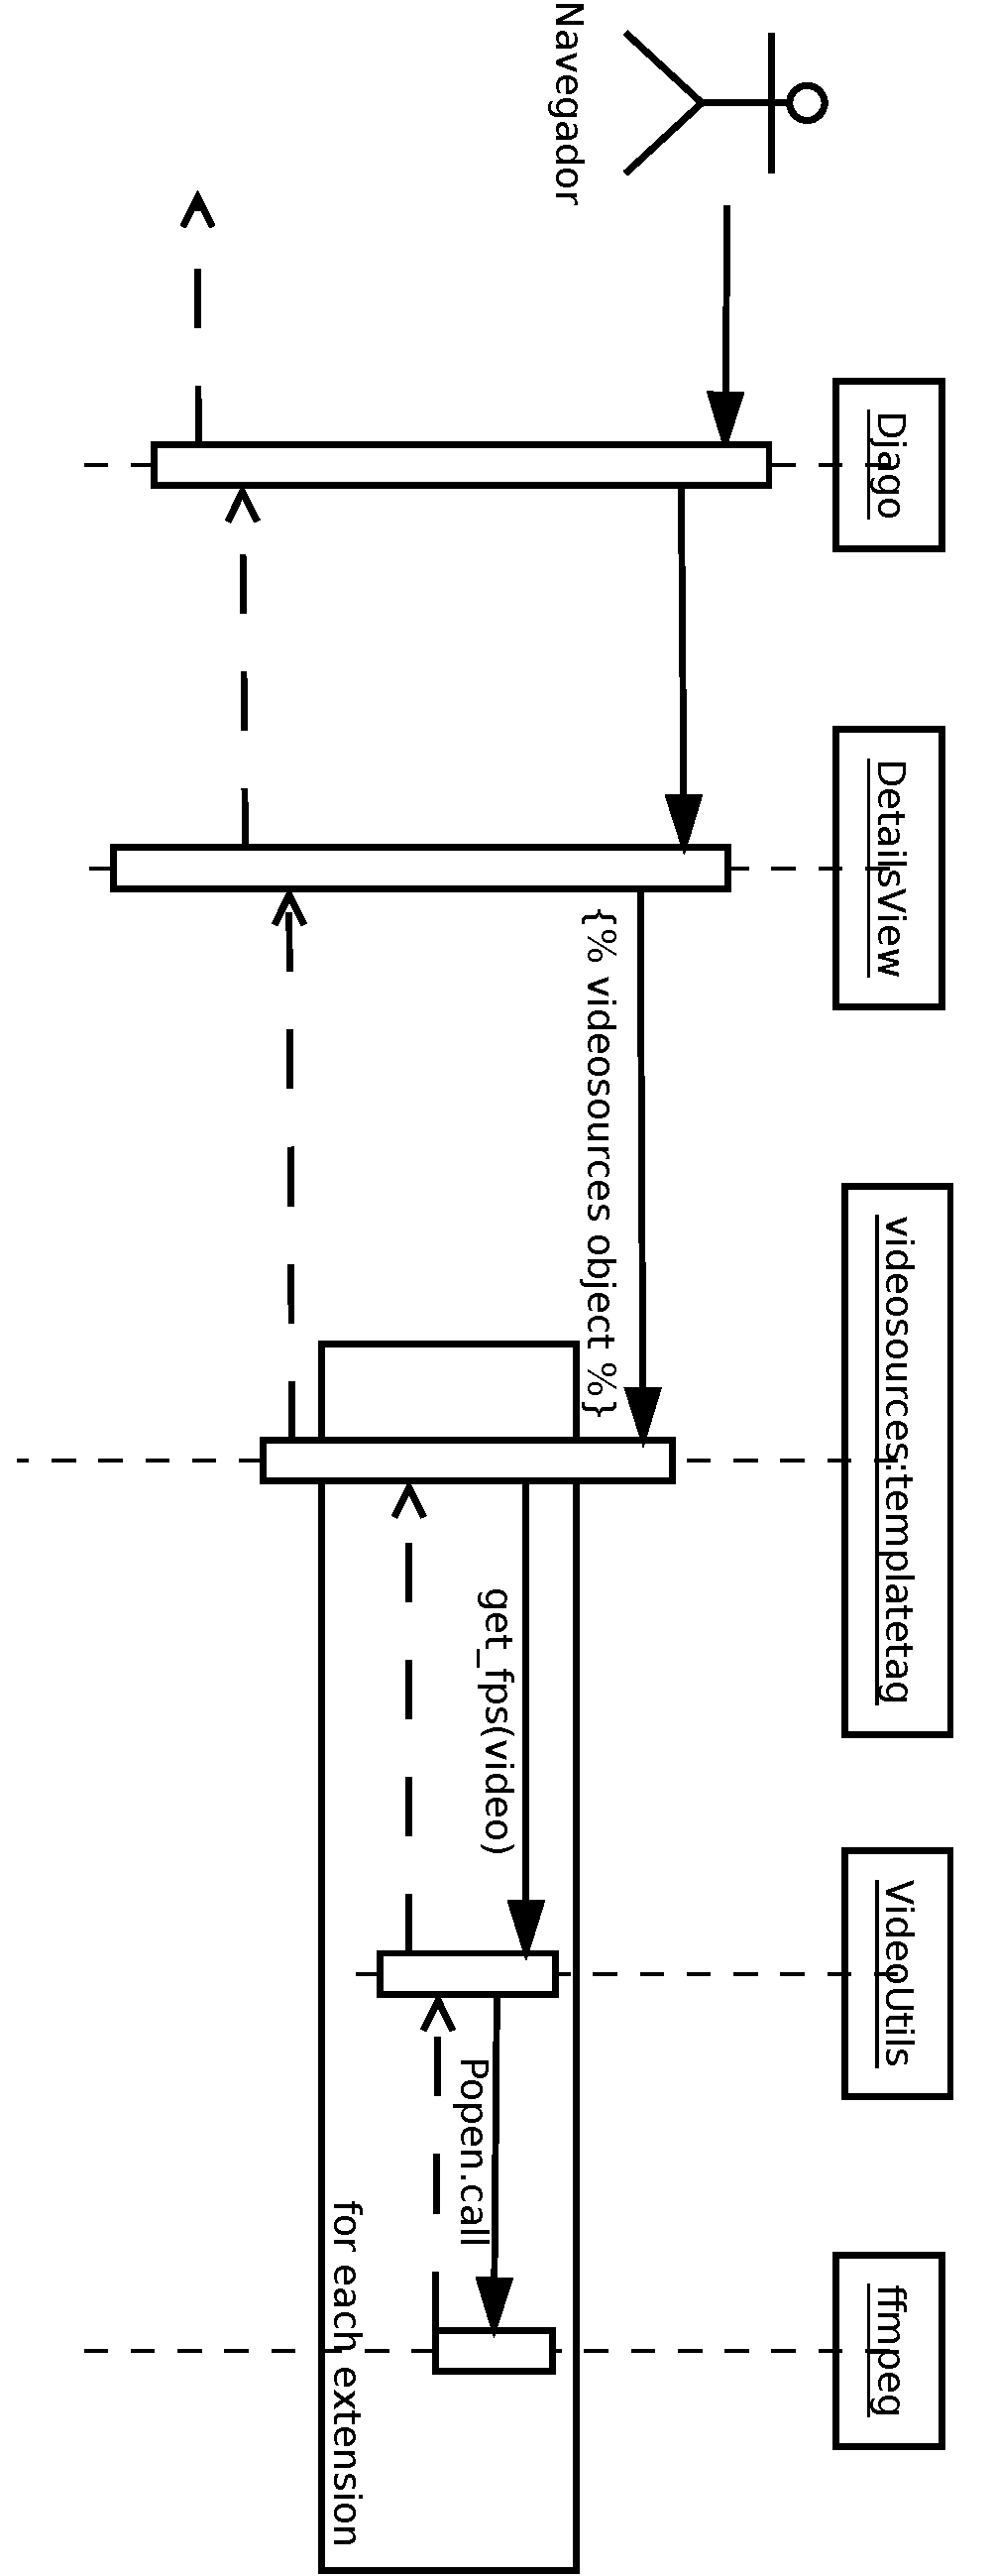
\includegraphics[scale=0.5]{figures/GenerateFpsDjango.pdf}
            \caption{Xeración do atributo fps no lado servidor}
        \label{fig:GenerateFpsDjango}
        \end{center}
        \end{figure}
                
        Coñecido pois o xeito no que refresca o estado da interface de usuario e o sistema que crea un 
        modelo obxectual para a representación gráfica das deteccións, agora compre ver como é que se 
        remarcan os obxectos detectados no vídeo. Isto faise mediante o elemento $<canvas>$ con
        id=``objects-canvas'' no que o observador da clase DetectedObjectsObserver encargase de debuxar
        un recadro da cor axeitada. Para coñecer esta cor que depende das opcións do panel o observador
        consulta a cada obxecto Detection empregando o método getCurrentColor() que se pode ver no 
        diagrama \ref{fig:DetectionClass}.

        
        \begin{figure}[htp]
        \begin{center}
            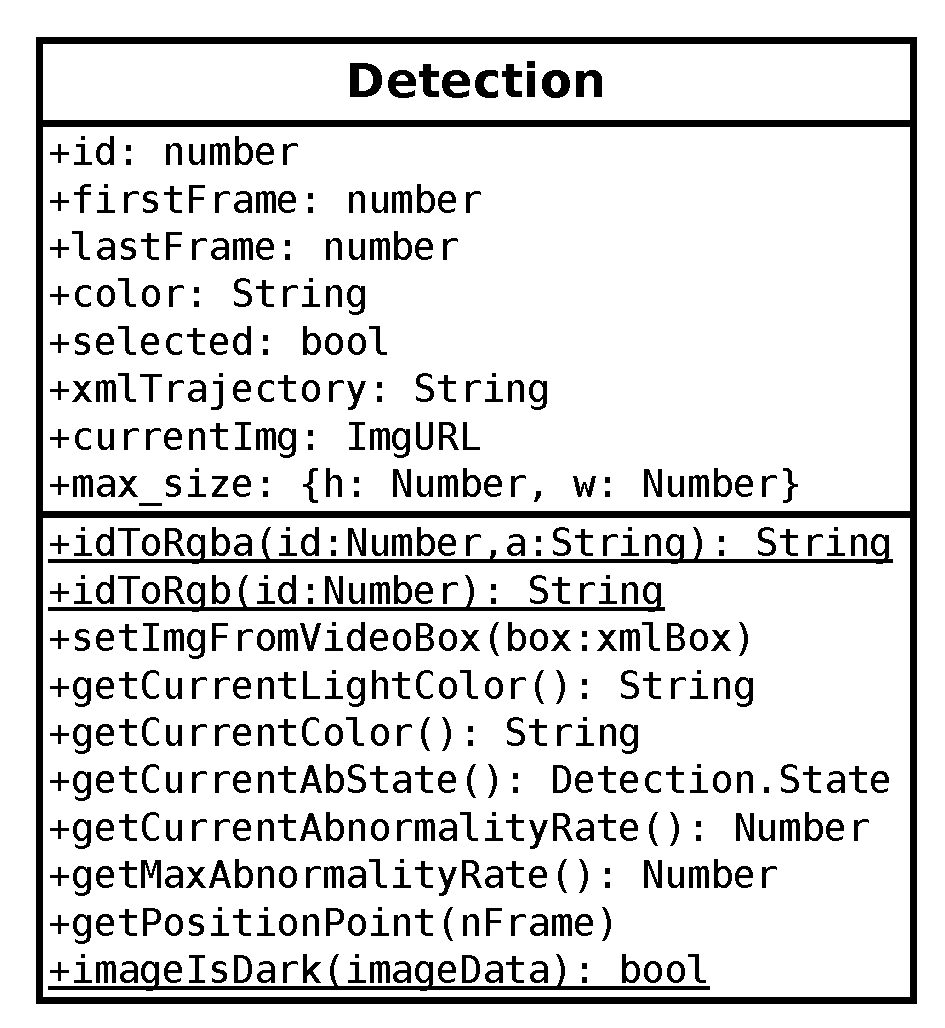
\includegraphics[scale=0.5]{figures/DetectionClass.pdf}
            \caption{Diagrama completo da clase Detection}
        \label{fig:DetectionClass}
        \end{center}
        \end{figure}
        
        Tamén cabe destacar aquí a función do observador TrainingMsgObserver, que é o encargado de 
        mostrar a etiqueta de Fotogramas de Adestramento e o recadro de cor amarelo nos primeiros 
        fotogramas do vídeo que corresponden aos empregados polo sistema de recoñecemento para obter o 
        fondo da imaxe e así poder distinguir os obxectos que se moven sobre el.
        
\section{v0.4 Arranxar bug's e mellorar a estratexia de probas}
    
    Esta versión estivo adicada a mellorar algúns aspectos transversais da aplicación que se 
    consideraban de importancia como a verificación e securización das páxinas web's que se detalla 
    con detalle no capítulo de Validación.
    
    \subsection{Re-analizar vídeo}
    En este sentido representa un incremento funcional 
        pequeno en comparación co acometido en outras iteracións, a funcionalidade mais destacable
        das elaboradas neste período foi a de Reanalizar o vídeo unha vez subido dende a páxina de 
        reprodución. Isto é moi útil no caso de que queiramos aplicar cambios ao sistema de 
        recoñecemento e ver velozmente como estes cambios afectan ao resultado da análise, xa que non é
        preciso volver a subir o vídeo á plataforma. O aspecto final desta funcionalidade pódese 
        ver na figura \ref{fig:reloadAnalysis}.
    
        \begin{figure}[htp]
        \begin{center}
            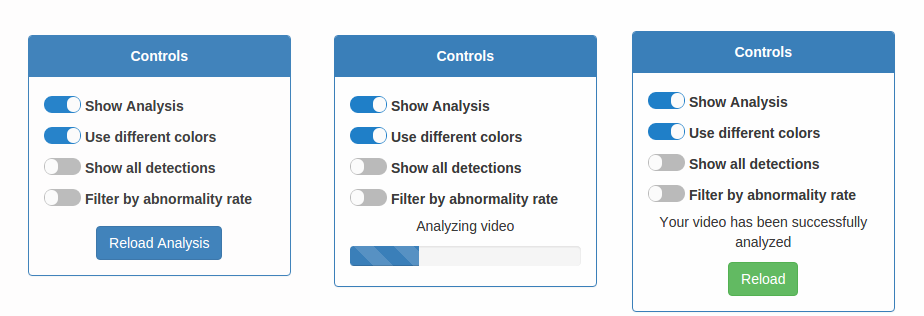
\includegraphics[scale=0.45]{figures/reloadAnalysis.png}
            \caption{Capturas de pantalla que amosan os distintos estados do botón de re-analise}
        \label{fig:reloadAnalysis}
        \end{center}
        \end{figure}

\section{v0.5 Traxectorias}
    As traxectorias son outra parte fundamental do sistema, debese mostrar a ruta seguida por 
    cada un dos obxectos detectados dende o momento no que entra en escena ata a súa saída. Para 
    que as traxectorias sexan detectadas no sistema de recoñecemento hai que invocar á biblioteca 
    de análise de alto nivel que require de unha cantidade de tempo considerable. É por elo que na 
    interface de liña de comando precisase un argumento de frecuencia que indique cada cantos 
    fotogramas se realizará a análise de alto nivel(por defecto cada 5 fotogramas).
    
    As traxectorias chegan á capa cliente como parte do XML resultado do sistema de análise, para 
    mostralas empregarase unha nova capa canvas en conxunto cun novo observador 
    TrajectoriesObserver que itera sobre as deteccións actuais pintando as liñas entre cada un dos
    puntos da súa ruta, dende o comezo desta ate o punto no que se atopa actualmente o obxecto. 
    Estes puntos son parseados polo obxecto Detection nada mais recibir o documento XML, quedando
    almacenados como parte do seu campo trajectory.
    
    Xa que a traxectoria forma parte da análise de alto nivel, e esta 
    non é executada en tódolos fotogramas, unha traxectoria estará composta por puntos que indican a
    posición do obxecto detectado con certa frecuencia (figura \ref{fig:calcTrajectory}).
    Para que entre un punto de detección e o seu
    seguinte pareza que hai avance, dando así sensación de fluidez, o que se fai é calcular dado o
    seguinte punto e o momento actual, cal é o lugar no que debería estar dito obxecto se se movese
    en liña recta entre ambos puntos, debuxando a liña da traxectoria ate esa posición calculada.
    
    \begin{figure}[htp]
    \begin{center}
        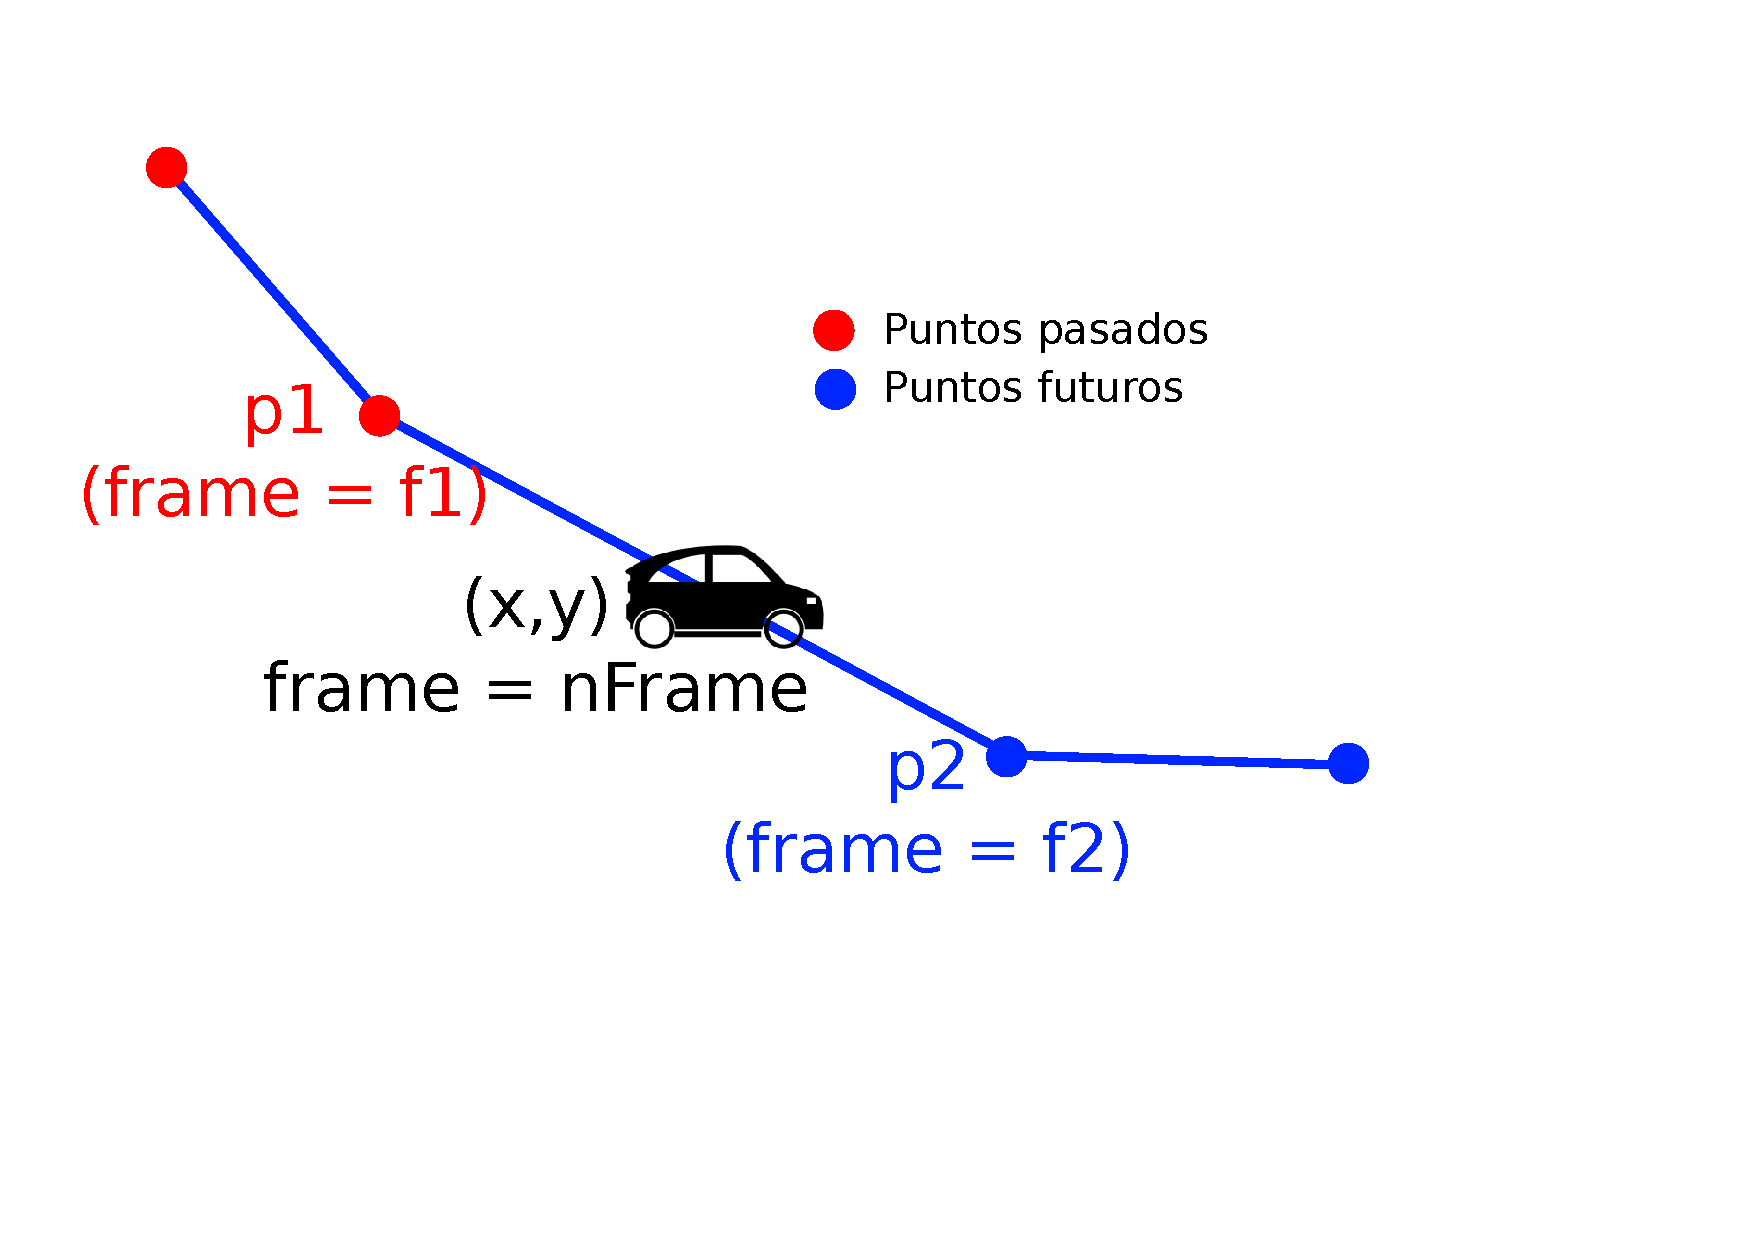
\includegraphics[scale=0.4]{figures/calcTrajectory.pdf}
        \caption{Diagrama do cálculo da traxectoria}
    \label{fig:calcTrajectory}
    \end{center}
    \end{figure}
    
    O cálculo realizase en base ao ``ratio'' que indica a distancia de entre os dous puntos que o coche 
    leva percorrido.
    
    \begin{verbatim}
        var ratio = Math.abs((nFrame - f1) / (f1 - f2));
        var x = p1.x + ratio * (p2.x - p1.x);
        var y = p1.y + ratio * (p2.y - p1.y);    
    \end{verbatim}
    
    Os resultados destes cálculos gárdanse para ser empregados en frames posteriores en caso de que
    sexa preciso.\\
    
    A parte das traxectorias, nesta iteración tamén se derou solución a outras funcionalidades como
    a támoa de Deteccións e a lista de deteccións actuais.

    \subsection{Táboa de Deteccións}

        Co fin de poder ollar todas as deteccións e podelas ordenar por orde de aparición, tempo en 
        escena, etc, crease unha táboa de obxectos detectados que ademais indica os obxectos que están
        a aparecer agora mesmo no vídeo, vexase figura \ref{fig:DetectionsTable}.
        A estes obxectos asígnaselle unha cor en función do seu 
        identificador unívoco, que ven xa composto por tres valores entre 0 e 255, e que se trata 
        segundo o model RGB como se mostra na figura \ref{fig:lightColor} para obter cores mais 
        brillantes e vistosas.
        
        \begin{figure}[htp]
        \begin{center}
            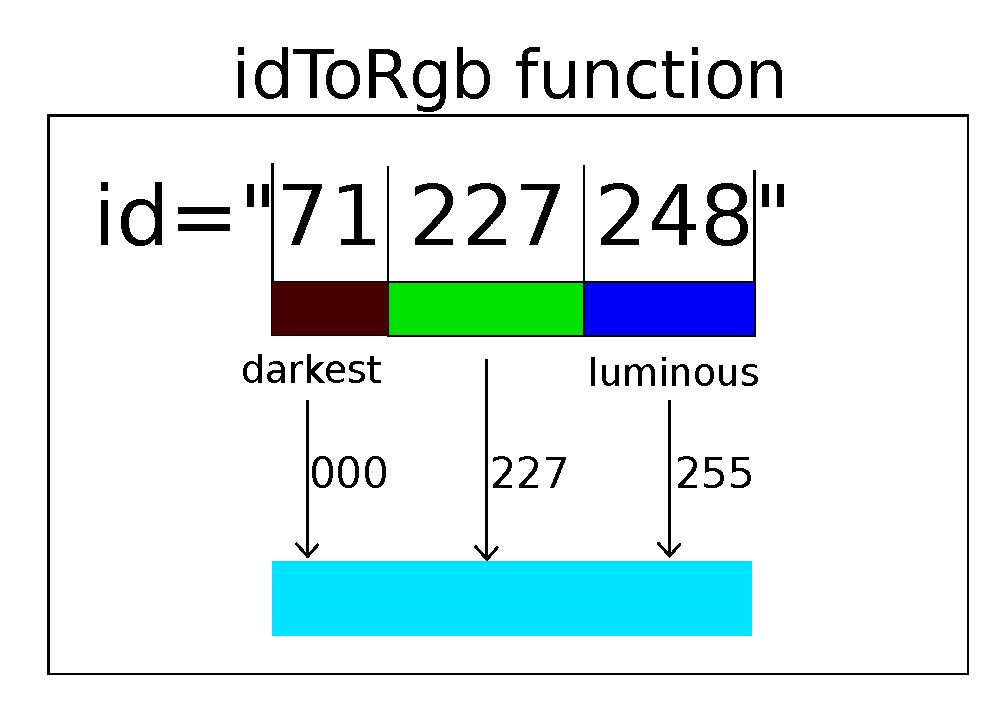
\includegraphics[scale=0.5]{figures/lightColor.pdf}
            \caption{Diagrama que mostra o aclarado de cores}
        \label{fig:lightColor}
        \end{center}
        \end{figure}

        Para o ordenamento da táboa empregouse a biblioteca javascript tablesorter que permite ordenar
        ascendente ou descendentemente a táboa facendo click na cabeceira do elemento polo que se desexa
        ordenar. Tamén é de destacar que os identificadores situados na primeira columna conteñen un 
        enlace que ao facer click leva o vídeo ao momento no que ese obxecto aparece por primeira vez en
        escena, función de tremenda utilidade á hora de recoñecelo.
        
        \begin{figure}[htp]
        \begin{center}
            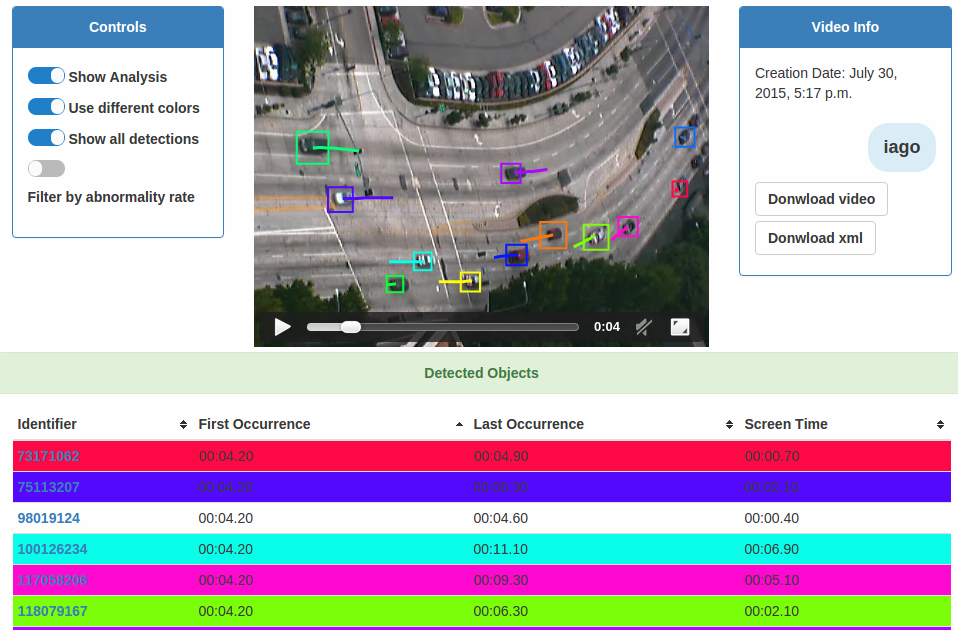
\includegraphics[scale=0.4]{figures/DetectionsTable.png}
            \caption{Captura de pantalla que amosa a táboa de obxectos detectados}
        \label{fig:DetectionsTable}
        \end{center}
        \end{figure}
        
        Como é lóxico esta táboa actualizarase en cada un dos fotogramas se hai algún novo obxecto 
        detectado ou se algún de eles desaparece, marcando ou desmarcando este como obxectos en escena.
        Este comportamento implementase mediante dúas listas no obxecto VideoDetections: 
        \textbf{detRecentlyDeleted} e \textbf{detRecentlySelected}, que son lidas polo observador 
        DetectionsTableObserver, encargado de remarcar todas as Deteccións da lista detRecentlySelected
        e de desmarcar todas as da lista detRecentlyDeleted, estas relacións entre as clases 
        VideoDetections e Detection pódense observar no diagrama \ref{fig:Detection-VideoDetections}.
        
        \begin{figure}[htp]
        \begin{center}
            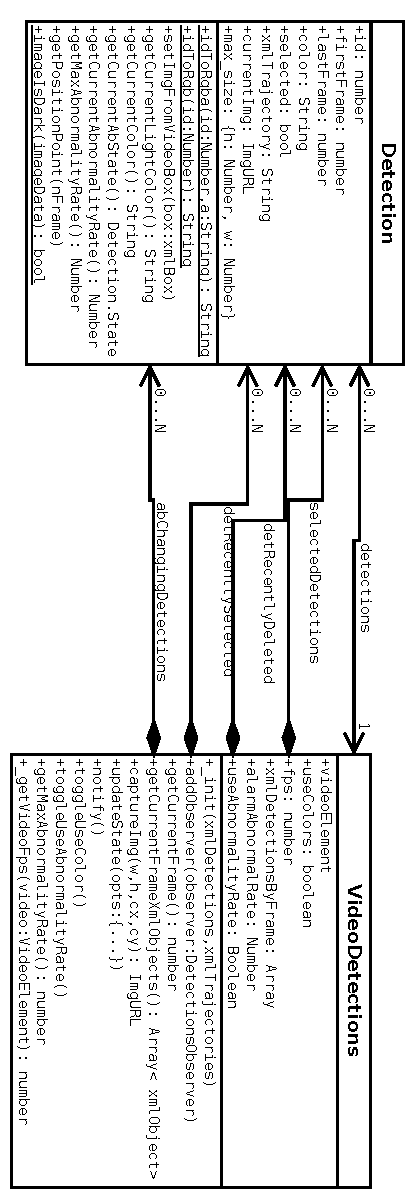
\includegraphics[scale=1]{figures/Detection-VideoDetections.pdf}
            \caption{Diagrama de clases que amosa detalladamente a relación entre as clases Detection
            e VideoDetections}
        \label{fig:Detection-VideoDetections}
        \end{center}
        \end{figure}
        
    \subsection{Lista de Deteccións actuais}

        Probablemente a función mais necesaria e vistosa é a de amosar os obxectos detectados de forma 
        individualizada mentres estes están en pantalla. A estes efectos crease unha lista de deteccións
        actuais que amosa unha imaxe de tódolos obxectos presentes no vídeo. O resultado pódese observar
        na figura \ref{fig:detectedObjects}.
        
        \begin{figure}[htp]
        \begin{center}
            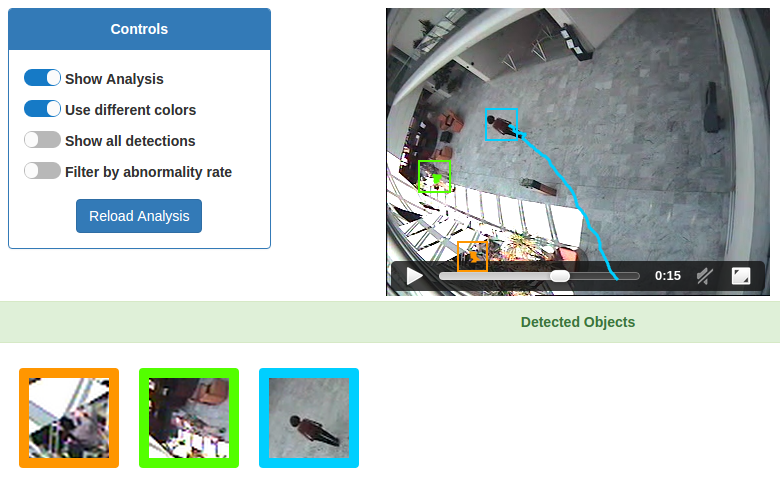
\includegraphics[scale=0.4]{figures/detectedObjects.png}
            \caption{Captura de pantalla que amosa a lista de obxectos detectados}
        \label{fig:detectedObjects}
        \end{center}
        \end{figure}
    
        Esta sección de deteccións actuais ao igual que a táboa de obxectos detectados precisa ser 
        actualizada en cada fotograma, para elo empréganse as listas de detRecentlyDeleted e 
        detRecentlySelected explicadas anteriormente, só que agora é o observador 
        CurrentDetectionsObserver o encargado de engadir ou borrar unha detección desta sección.
        
        Tamén hai que destacar que xa que os observadores CurrentDetectionsObserver e 
        DetectionsTableObserver son os que mais tempo de execución consumen, a súa execución é 
        complementaria dependendo do estado do checkbox ``Show all detections''. De estar
        deshabilitado mantén o observador DetectionsTableObserver inactivo mentres que o 
        CurrentDetectionsObserver está activo, e estando habilitado fai o contrario. Isto obriga aos
        observadores a reimplementar os métodos ``enable()'' e ``disable()'', cargando ou
        descargando nestes métodos todos os valores actuais das deteccións que non actualizaron mentres
        estaban deshabilitados.
        
        As imaxes que se amosan como icona de cada un dos obxectos detectados son calculadas en tempo de
        reprodución do vídeo, isto é posible grazas aos elementos data URI\cite{data-uris} de javascript,
        que permiten almacenar unha imaxe como se fose unha URL e empregar esta URL para logo mostrar a 
        imaxe, por poñer o caso, no fondo (background-image) de un elemento HTML. Esta URI calcúlase 
        no método da clase VideoDetections ``captureImg'' empregando unha chamada a ``canvas.toDataURL()''
        onde canvas é un elemento HTMLCanvasElement obtido a partir do fotograma actual do vídeo.
        
        Por último para mostrar a información asociada a este obxecto detectado de algún xeito, 
        empregase a compoñente da librería bootstrap popover, que é unha ventá flotante que xurde ao
        carón da detección cando o rato pasa por enriba dela. Este popover personalizase coa cor 
        concreta desa detección (ver figura \ref{fig:popoverCapture}).
        
        \begin{figure}[htp]
        \begin{center}
            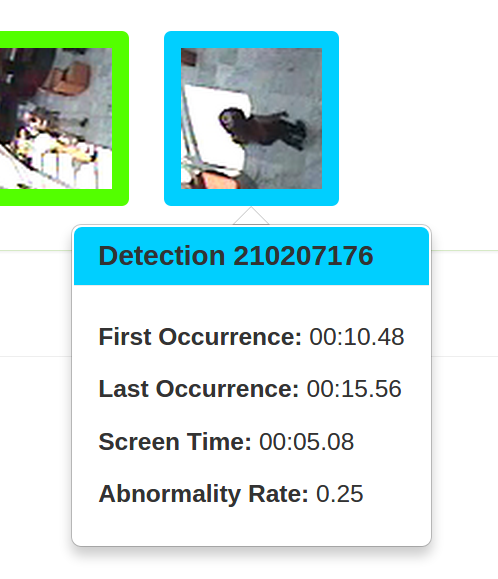
\includegraphics[scale=0.5]{figures/popoverCapture.png}
            \caption{Captura de pantalla que amosa o popover da lista de deteccións actuais}
        \label{fig:popoverCapture}
        \end{center}
        \end{figure}
        
    
\section{v0.6 Detección do comportamento anómalo}
    
    Un dos factores nos que destacan os algoritmos dos laboratorios VARPA é precisamente a análise
    de comportamento co fin de detectar o comportamento anormal de un dos obxectos implicados nunha
    escena. Isto faise calculando cal é o camiño polo que un obxecto soe viaxar do punto A ao 
    punto B, para calquera que sexan os puntos A e B, de xeito que podemos medir o anormal que é
    o seu comportamento en función do que o seu camiño se diferencie do camiño habitual. Isto pode
    axudar a detectar por exemplo un peón que non cruza polo paso de cebra, un coche facendo unha 
    manobra perigosa...
    
    O sistema de recoñecemento facilitado polo laboratorio foi deseñado para poder devolver un ratio
    de esa anormalidade en cada unha das chamadas ao sistema de análise de Alto nivel, que como se 
    dixo anteriormente executase cada determinado período de tempo. E dado que é este sistema o que
    proporciona a traxectoria do obxecto, o ratio de anormalidade para cada un dos momentos 
    asociouse pois a cada un dos puntos da traxectoria como se pode ver na imaxe \ref{fig:abXmlRate}.
    Como se pode comprobar nesta imaxe, existen unha serie de momentos iniciais nos que o ratio inda
    non puido ser calculado, e neste caso o valor asociado será 0.
    
    \begin{figure}[htp]
    \begin{center}
        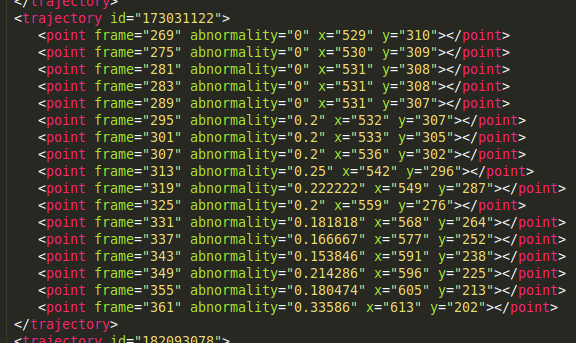
\includegraphics[scale=0.5]{figures/abXmlRate.png}
        \caption{Ratio de anormalidade gardado nun documento XML}
    \label{fig:abXmlRate}
    \end{center}
    \end{figure}
    
    Non obstante un número é algo moi pouco gráfico, que dificilmente pode axudar a resaltar unha 
    detección anómala de unha que non o é, por este motivo se deseñou unha serie de compoñentes que
    permiten seleccionar un límite (un ratio de anormalidade máximo) a partir do cal un obxecto será
    considerado sospeitoso. A nivel de interface web, este límite pode marcarse cunha barra 
    selectora chamada slider, que  se importou da libraría jQuery UI\cite{ComponenteSliderJqueryUi},
    e que se complementou cunha entrada de texto para dar a posibilidade de que o valor se seleccione
    ou ben escribíndoo, ou ben a través do slider (vexase figura \ref{fig:sliderCapture}).
    Os valores a seleccionar variarán sempre entre 0 e o máximo valor atopado entre os ratios de
    anormalidade das deteccións.

    \begin{figure}[htp]
    \begin{center}
        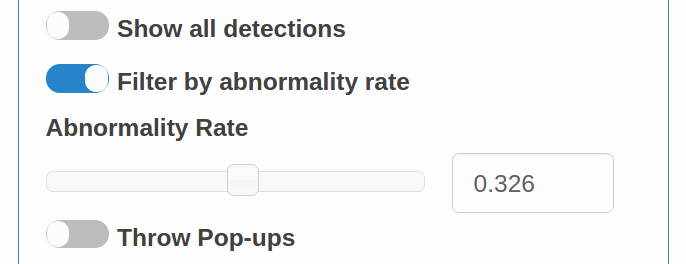
\includegraphics[scale=0.5]{figures/sliderCapture.png}
        \caption{Captura de pantalla do compoñente slider da biblioteca jQuery UI}
    \label{fig:sliderCapture}
    \end{center}
    \end{figure}
    
    Agora que xa se pode seleccionar o valor a partir do cal queremos marcar unha detección como
    anómala, falemos do xeito no que se vaia realizar este marcado. A idea xeral consiste en 
    inabilitar o uso de diferentes cores e marcar de azul todas as deteccións, con excepción de 
    aquelas que teñan un comportamento anormal que serán marcadas de vermello, e aquelas cuxo 
    comportamento inda non fose analizado que serán marcada en cor negra como se pode ver na imaxe
    \ref{fig:suspiciousDetections}. Este uso de cores no só
    se emprega nas capas $<canvas>$ de información que se amosan sobre o vídeo senón tamén na táboa
    de obxectos detectados e na lista de deteccións actuais.

    \begin{figure}[htp]
    \begin{center}
        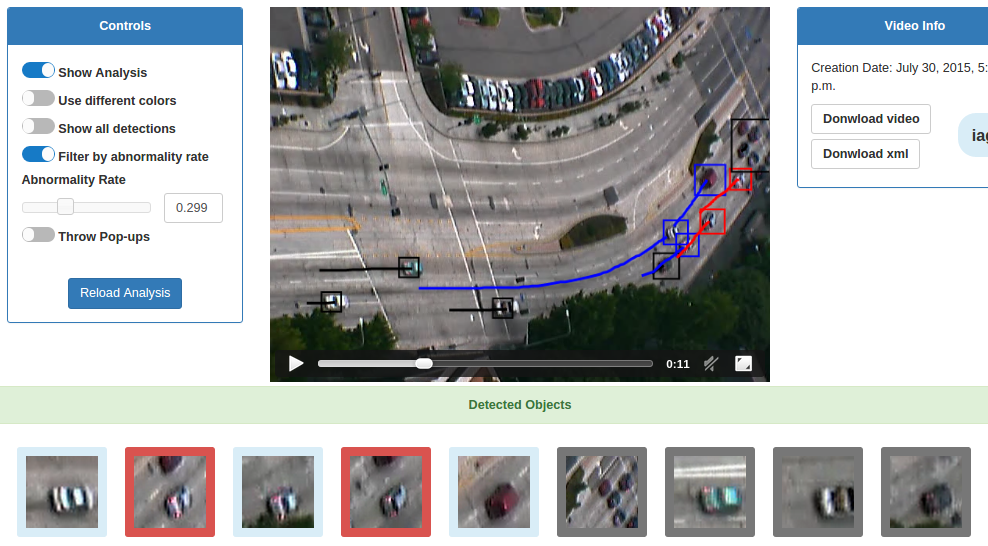
\includegraphics[scale=0.4]{figures/suspiciousDetections.png}
        \caption{Captura de pantalla que amosa o comportamento das deteccións sospeitosas}
    \label{fig:suspiciousDetections}
    \end{center}
    \end{figure}
    
    Para conseguir isto, centralizase a xestión da cor sobre o obxecto Detection que se pode ver en
    detalle no diagrama \ref{fig:DetectionClass}, facendo que sexa 
    este o que determine de forma unívoca de que cor se ten que debuxar. Para isto creanse os 
    métodos ``getCurrentColor'' que devolve a cor para as capas $<canvas>$ e 
    ``getCurrentLightColor'' que devolve un color mais claro para a táboa e a lista de deteccións.
    O obxecto Detection á súa vez calculara a cor a devolver en función do seu ratio de anormalidade
    e o valor das propiedade: videoDetections.alarmAbnormalRate, videoDetections.useAbnormalityRate
    e videoDetections.useColors.
    
    A parte deste mecanismo para centralizar a xestión do color que será empregado por tódolos 
    observadores, os observadores DetectionsTableObserver e CurrentDetectionsObserver precisan 
    coñecer aquelas deteccións que cambiaron a un estado sospeitoso, de confianza ou sen datos,
    con este obxectivo crease a lista VideoDetections.abChangingDetections (ver diagrama 
    \ref{fig:Detection-VideoDetections}), que indicará aquelas
    deteccións que cambiaron de estado e polo tanto, no caso da táboa e a lista de deteccións, 
    precisan mudar a súa cor.
    
    \subsection{Popups de deteccións sospeitosas}

        Para completar a funcionalidade de detectar o comportamento anómalo, solicitase unha faceta a 
        maiores do marcado das deteccións sospeitosas, deberase dar a opción de lanzar unha nova ventá
        por cada obxecto sospeitoso detectado coa posibilidade de ver este obxecto de preto ao largo do
        seu percorrido.
        
        Tras estudar varios xeito de facer isto, a mellor solución parece ser a de empregar pop-ups 
        tamén chamados ventás emerxentes, que inda que normalmente se evitan por estares asociados 
        con contido publicitario, neste caso compren á perfección coa tarefa que se desexa realizar.
        
        Xa que haberá que ampliar a imaxe facendo un efecto zoom para poder mostrar a zoa do vídeo na
        que está a detección con mais detalle, prantexase a construción dun sistema que mediante unha
        barra selectora (slider) permita achegarse ou afastarse para ver mais de preto ou de lonxe o 
        obxecto detectado. Para estas ventás emerxentes empregarase un novo ficheiro .css e tamén un 
        novo ficheiro .js, que conterá os mecanismos precisos para crear este efecto zoom.
        
        A esta nova ventá pasaranse como parámetros da URL o identificador da detección e a ULR do 
        ficheiro XML que contén a análise. Con estes datos o ficheiro javascript principal chamado
        suspicious-popup.js, que segue unha distribución similar ao de video-player.js para a páxina
        que amosa o vídeo, obterá o ficheiro XML e en base a el iniciará o sistema. Esta
        páxina tamén constará dun elemento $<video>$, con capas $<canvas>$ superpostas, a primeira delas 
        ocultará o vídeo por completo mostrando a porción del que sexa precisa para lograr o efecto 
        zoom e as sucesivas mostrarán a información desexada.
        
        Ao manter a estrutura dun elemento $<video>$ coas capas $<canvas>$ superpostas, a mellor 
        arquitectura posible e a dun patrón Observador, no que o suxeito manteña ademais das referencias
        ao vídeo, os datos sobre o nivel de zoom, que será necesariamente empregado polos seus 
        observadores. Para esta tarefa reempregouse gran parte do deseño do diagrama \ref{fig:observerPattern}
        engadindo as características precisas nunha clase herdada de VideoDetections que se nomea 
        ZoomVideoDetections como se pode ver na figura \ref{fig:SuspiciousPopupJS}.
        
        \begin{figure}[htp]
        \begin{center}
            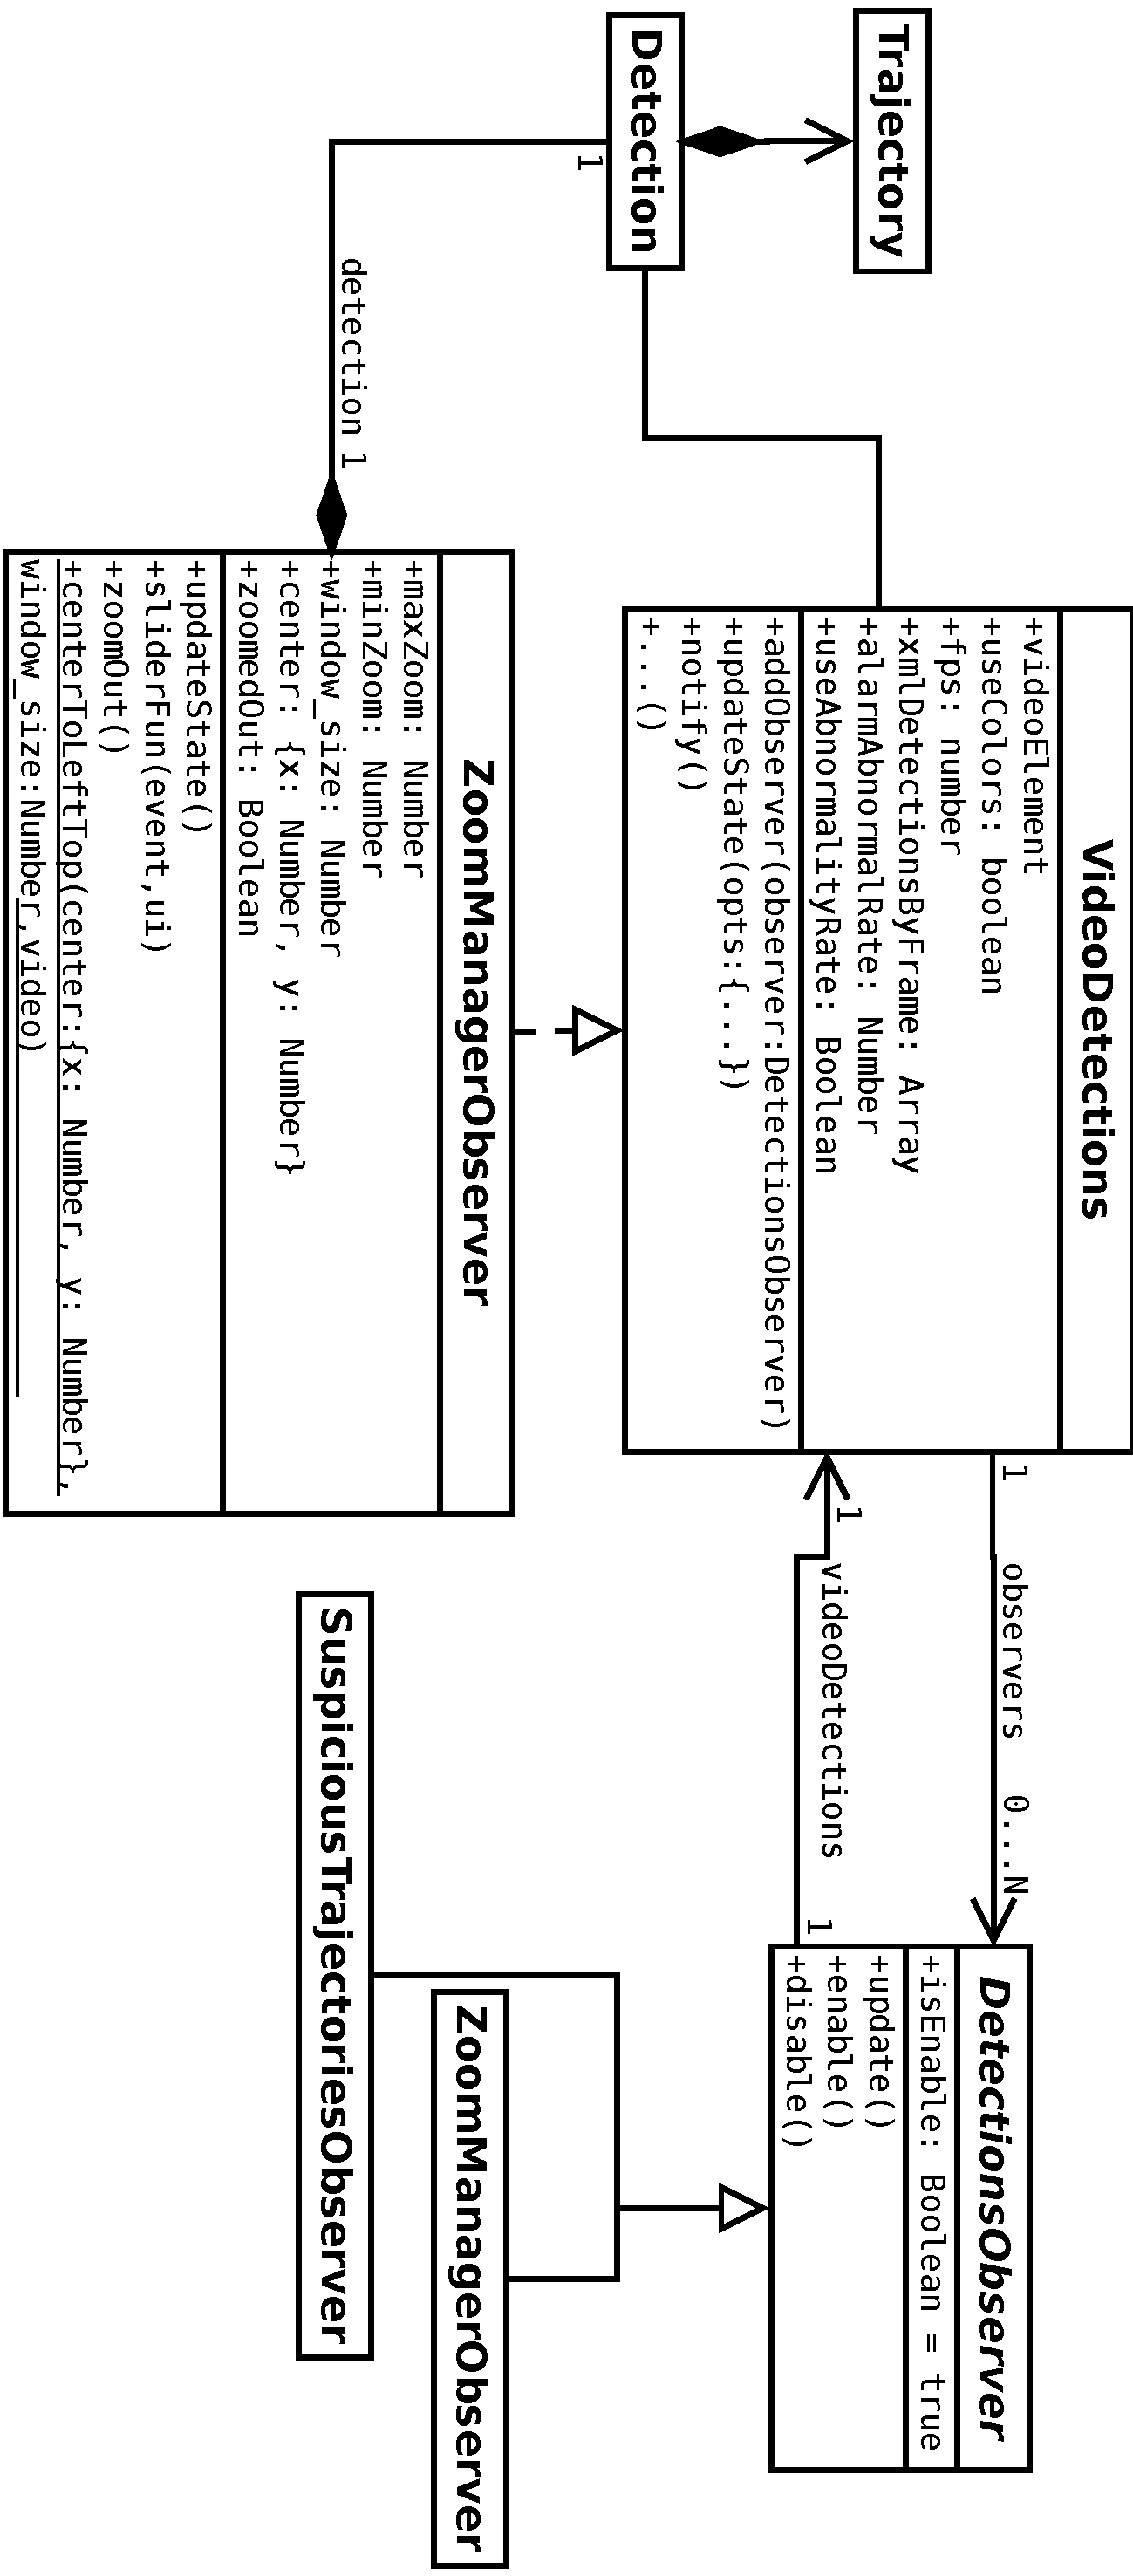
\includegraphics[scale=0.45]{figures/SuspiciousPopupJS.pdf}
            \caption{Diagrama de clases simplificado para a ventá emerxente de deteccións sospeitosas}
        \label{fig:SuspiciousPopupJS}
        \end{center}
        \end{figure} 
        
        Este sistema é iniciado na carga do XML e ao igual que na páxina que reproduce o vídeo, cando a 
        carga finaliza crease
        un bucle coa función updateStatus que actualizará en cada fotograma o estado dos compoñentes 
        chamando á función ZoomVideoDetections.updateState(). Esta función tamén é chamada cando o vídeo
        lanza o evento play, ou ao cambiar o nivel de zoom mediante a barra selectora (slider).
        O resultado final, mostrase quedou como se pode ver na figura \ref{fig:suspiciousPopupCapture}.

        \begin{figure}[htp]
        \begin{center}
            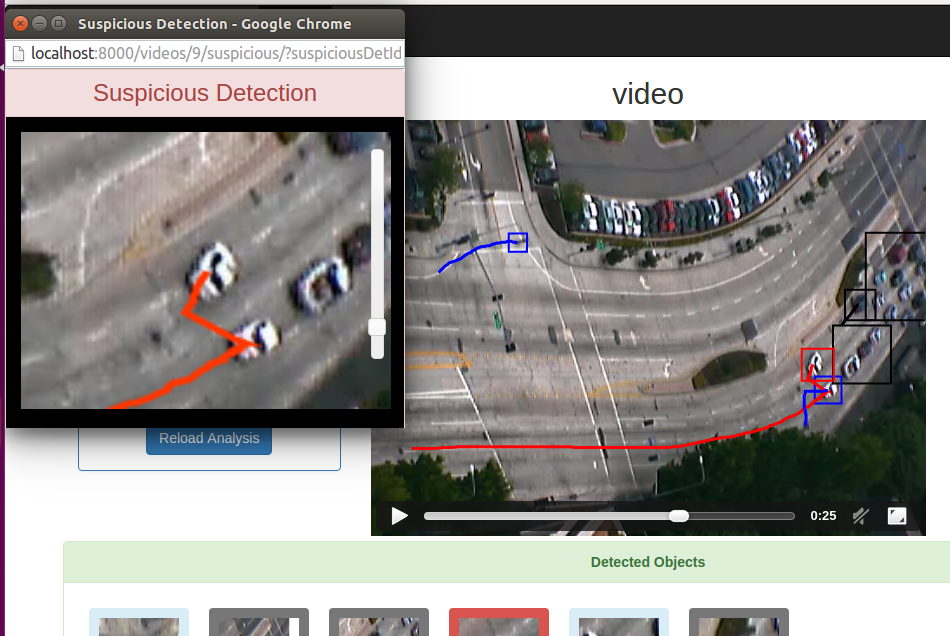
\includegraphics[scale=0.4]{figures/suspiciousPopupCapture.png}
            \caption{Captura de pantalla que amosa a ventá de deteccións sospeitosas}
        \label{fig:suspiciousPopupCapture}
        \end{center}
        \end{figure} 
        
        A continuación explicase en detalle o mecanismo empregado para crear o efecto zoom e para 
        levar a cabo o seguimento do obxecto mantendo este nivel de zoom. Empréganse 
        basicamente dúas variables, por un lado o tamaño da fracción de vídeo a amosar (w\_size), que
        variará entre un mínimo(dúas veces o tamaño da detección) e un máximo que é o tamaño do vídeo, 
        e por outro lado o centro (center) da escena que será unha variable composta de dúas 
        compoñentes (x,y) que indican a distancia en píxeles á parte superior esquerda do vídeo.
        
        A función ZoomVideoDetections.centerToLeftTop é a encargada de calcular dado un tamaño de ventá 
        e un centro, esta distancia á marxe esquerda superior do vídeo. Este cálculo no é sinxelo, xa que 
        hai que evitar que o recadro a seleccionar exceda das dimensións do vídeo. Esta casuística 
        amosase na figura \ref{fig:centerToLeftTop}.
        
        \begin{figure}[htp]
        \begin{center}
            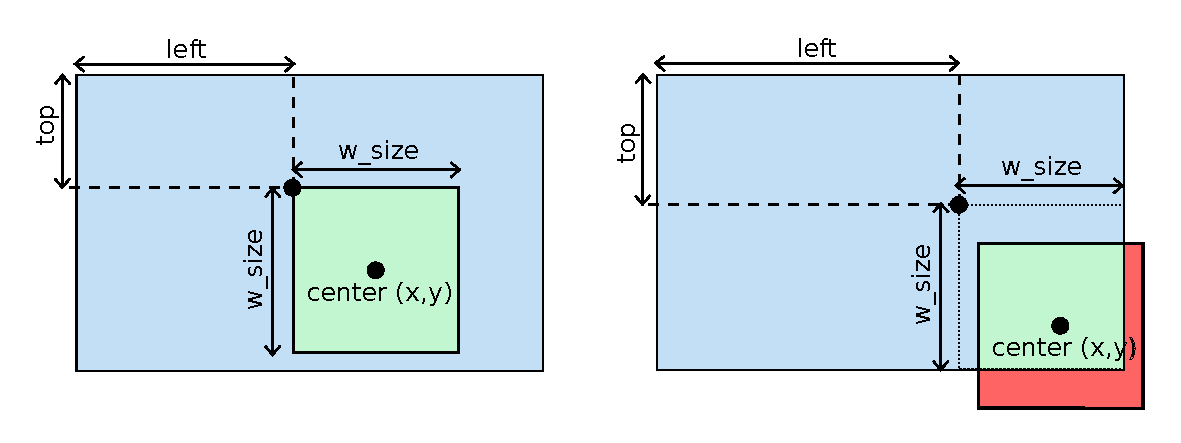
\includegraphics[scale=0.75]{figures/centerToLeftTop.pdf}
            \caption{Diagrama que explica os problemas resoltos para implementar o efecto zoom}
        \label{fig:centerToLeftTop}
        \end{center}
        \end{figure}

\section{v1.0 Memoria e posta en produción}
    Esta última fase adicouse principalmente a completar a memoria, a solucionar pequenos problemas
    acumulados nas anteriores versións e á publicación de esta aplicación baixo un entorno de 
    produción.
    
    Para a publicación desta aplicación web, realizarase a súa montaxe sobre un servidor on-line,
    é dicir, unha máquina conectada a internet que dispón de conexión directa a unha dirección IP
    fixa, e a capacidade para manterse en funcionamento de forma continua. A esta IP referenciará un
    servidor DNS, que se contratará xunto co dominio \url{www.ancoweb.es} a través do cal poderase
    acceder á páxina.

    \subsection{Dominio}
        O dominio ten que ser rexistrado cos datos da persoa responsable, neste caso o autor do 
        proxecto, a través dunha empresa rexistradora. Seleccionase a empresa 1\&1
        \cite{1and1-website} xa que tamén oferta servizo DNS(Domain Name System) para apuntar ao 
        servidor que contén a aplicación.
        
        Unha vez creado o dominio, a única configuración a establecer para que este funcione 
        é a dirección do servidor, que indicaremos no rexistro de tipo A como se pode
        ver na figura \ref{fig:1and1Capture} onde a dirección IP do servidor é 45.55.51.164.

        \begin{figure}[htp]
        \begin{center}
            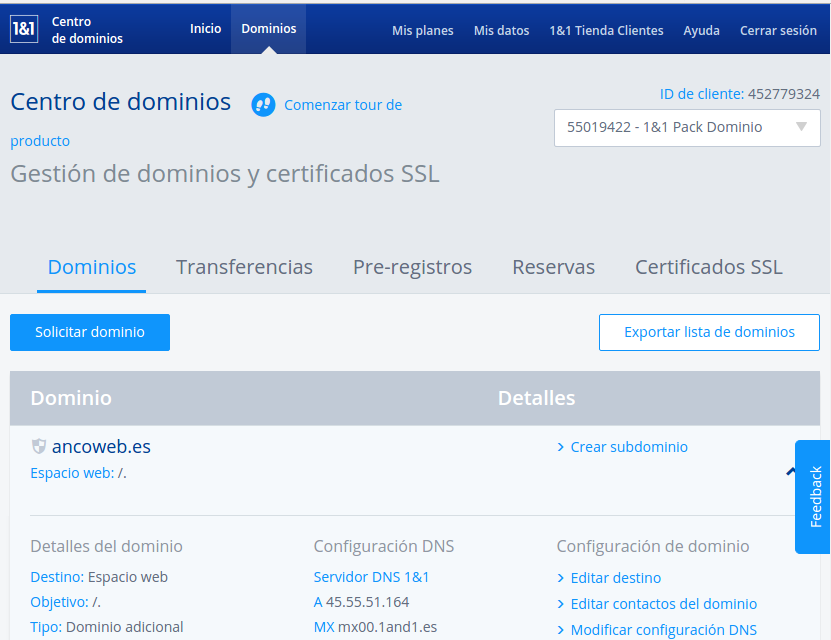
\includegraphics[scale=0.5]{figures/1and1Capture.png}
            \caption{Panel de control da ferramenta 1and1}
        \label{fig:1and1Capture}
        \end{center}
        \end{figure}
    
    \subsection{Hosting}
        Na dirección IP 45.55.51.164 reside o servidor montado para distribuír a aplicación web a 
        todo aquel que se conecte. Este servidor pertence á empresa DigitalOcean
        \cite{digitalocean-website} que se seleccionou de entre outros servizos de hosting por 
        permitir a posibilidade de crear o entorno de produción dende zero, podendo así instalar 
        todos os paquetes preciso para a integración das múltiples tecnoloxías implicadas neste 
        proxecto.
        
        Neste caso seleccionouse como punto de partida unha máquina Ubuntu Server 14.04 con 1GB de 
        memoria RAM, un só núcleo de CPU e 30GB de memoria SSD, todo elo localizado en Nova York.
    
    \subsection{Configuración do Servidor}
        A partir da base que nos proporciona DigitalOcean, que é unha máquina Ubuntu Server 14.04 
        completamente limpa, pódese seguir a guía contida no ficheiro production-README.md situado
        na base do proxecto que indica con detalle todos os comandos a executar para una correcta 
        configuración. 
        
        Como peza central escolleuse o servidor Apache2, este servidor será o encargado de servir 
        tódolos arquivos, tanto páxinas web como ficheiros multimedia e recursos da aplicación. Mais
        este servidor de por si só, non pode executar o framework de Django que se precisa para 
        atender as peticións dos clientes, co que se engade un módulo chamado mod\_wsgi
        que permite executar código python sobre o servidor mediante o ficheiro do proxecto
        ``src/ancoweb/wsgi.py''. A dificultade especia está en configurar adecuadamente todo o entorno
        para executar Python 3.4, pois é unha versión soportada por mod\_wsgi recentemente.
        
    \subsection{Axustes de Produción}
        En produción existen toda unha serie de parámetros que cambian en relación co entorno de 
        desenvolvemento, para soportalos creouse un novo ficheiro de configuración que herda do 
        anterior chamado ``settings\_production.py'' e que está situado no directorio 
        ``/src/ancoweb''.
        
        Para indicar ao sistema que empregue este ficheiro en lugar de settings.py, o que se fixo 
        foi modificar o ficheiro ``src/ancoweb/wsgi.py'' facendo que este apunte ao ficheiro de 
        produción en lugar de ao de desenvolvemento, así cada vez que o proxecto se execute mediante
        mod\_wsgi empregaranse os axustes de produción, e en caso contrario os axustes por defecto.
        
        Un dos axustes de configuración mais importantes é o da variable STATIC\_ROOT, esta indica
        onde se almacenarán os recursos da aplicación, e neste caso decidiuse empregar o directorio
        ``/var/www/static/'' polo que antes de ser despregada todos o recursos precisos de tódalas 
        aplicacións incluídas deben ser movidos a este directorio empregando o comando:
        
        \begin{verbatim}
        sudo python manage.py collectstatic 
            --settings=ancoweb.settings_production
        \end{verbatim}

        O outro axuste de gran interese é o lugar no que se almacenan os ficheiros multimedia, pois
        a meirande parte da aplicación xira en torno a eles. Neste caso a variable en conflito é 
        MEDIA\_ROOT, que no caso do entorno de produción tomará o valor ``/var/www/media/'', e en 
        caso de estar en desenvolvemento ``MEDIA\_ROOT = str(BASE\_DIR / 'media/')''. Isto obriga ao 
        igual que cos recursos do proxecto a mover os arquivos multimedia cada vez que se desexe 
        despregar a aplicación, neste caso co comando:
        
        \begin{verbatim}
        sudo cp -R ancoweb-TFG/src/media/ /var/www
        \end{verbatim}

\chapter{Validación}

Á hora de deseñar probas é importante abarcar a maior parte do código posible, neste proxecto isto
foi todo un reto, pois o alto nivel de integración dificulta enormemente a realización das probas.
Pese a todo, logrouse probar tanto o código realizado en Python-Django así como o código da capa 
cliente en javascript, empregando para elo distintos modelos e bibliotecas de probas que vemos a
continuación.

\section{Probas Unitarias}

    As probas unitarias proban as funcionalidades mais básica do software. Executanse sempre no 
    ámbito de un só modulo para probar o correcto funcionamento de este, simulando se fose preciso 
    a súa interacción con outros módulos (este proceso chamase mocking).
    
    No ámbito da nosa aplicación as probas de cada módulo recollense nos ficheiros tests.py de cada
    un deles. Estas probas inclúen tanto comprobacións de funcións illadas, como a correcta xeración
    de algunha webs independentes do resto dos módulos.
    
    \subsection{Política de acceso ás páxinas web}
        Como resulta lóxico non todo o mundo pode acceder a tódalas páxinas da aplicación, algunhas
        delas están reservadas para o administrador, outras para o propio usuario logueado, unhas
        terceiras para calquera usuario logueado e por último hai páxinas de dominio público.
        
        É importante de cara a non cometer erros de seguridade, que este correcto comportamento sexa
        comprobado, así na táboa excel que se atopa no ficheiro docs/urlsMap.ods pódese observar con
        detalle que política de acceso segue cada unha das páxinas da aplicación segundo a súa URL.
        Foi a partir deste mapa de urls dende onde se elaborou a base dos test de unidade para 
        o acceso ás páxinas, que comprobar para cada unha das páxinas da aplicación que un usuario
        cos permisos adecuados poida acceder e que calquera dos demais reciba o erro axeitado.
        
        Pero só con probas unitarias non se pode asegurar a calidade dos software xa que moitos dos
        módulos están pensados para interactuar entre eles, polo que fanse necesarias as Probas de
        Integración.

    \subsection{Probas da Capa Web con Javascript}
        As probas da capa web en escrita en javascript apoiaranse no framework Qunit de 
        jQuery que proporciona un xeito sinxelo de crear probas unitarias sempre e cando o código 
        javascript esté convintemente separado do HTML que forma a vista da capa web.
        
        Como resulta lóxico, estas probas estarán escritas en javascript e almacenadas no directorio
        do proxecto /src/static/site/tests, podendo executarse de dous xeitos diferentes: Ou ben 
        como unha páxina web pertencente á aplicación (isto favorece o desenvolvemento áxil), ou ben
        como unha proba das realizadas polo comando python manage.py test.
        
        Para poder executar un código javascript dende a execución común dos tests da aplicación, 
        precisamos un lanzador ou runner que lance estes tests contra algún navegador de liña de 
        comandos, neste caso a opción seleccionada foi a combinación do paquete django.js (v0.8.1)
        en combinación co navegador de liña de comandos phantomJS. 
        
        Django.js é un conxunto de utilidades que permiten a integración de código javascript en 
        Django. Mais en concreto neste proxecto empréganse aquelas que teñen que ver co testing de
        aplicacións \cite{DjangojsTestTools}, destacando as clases QUnitSuite e PhantomJsRunner que se
        empregan para lanzar os tests como parte dos test da aplicación mediante a clase creada
        StaticJsTestCase que obtén os resultados do modo de páxina web co navegador de liña de 
        comandos, e tamén a clase QUnitView que é a peza central para a execución a neste modo de
        páxina web.
        
        Po outro lado PhantomJS é un navegador WebKit de liña de comandos, cunha API Javascript que
        da soporte rápido e nativo para varios estándares web que resultan moi do noso interese,
        como son a manipulación DOM, os selectores CSS, JSON, Canvas e SVG. PhantomJS será chamado
        implícitamente polo runner de Django.js cando se executen os test, mentres que no caso da 
        vista QUnitView os tests executaranse directamente no navegador que realice a petición.

\section{Probas de Integración}

    As probas de integración so aquelas que proban o funcionamento conxunto de varios módulos da 
    aplicación, realizanse tras o éxito das probas unitarias tamén sen que haxa interacción humana.
    
    No noso caso agruparemos as probas de integración nun paquete a parte, para evitar así 
    mesturalas coas probas unitarias de cada módulo. A estes efectos creamos a clase SeleniumAncowebTest
    que extende StaticLiveServerTestCase engadindo ademais os métodos login\_user(self, user, 
    password) e logout\_user(self, user) xa que todo-los tests que comproben outros módulos precisando
    de un usuario logueado consideranse tests de integración.

    \subsection{Probas Funcionais Selenium}

        As probas funcionais son aquelas nas que se lle dita ao sistema cales serán as saídas a unha 
        determinada serie de entradas co fin de comprobar que a funcionalidade é a correcta. No caso da
        nosa aplicación empregaremos tests funcionais para as probas de integración apoiandonos en Selenium.
        
        Selenium é un framework para a realización de probas funcionais que permite lanzar un navegador
        e indicar as accións a realizar sobre él xunto cunha serie de comprobacións para verificar que
        estas accións provocan na páxina web o efecto desexado. Resultan de especial relevancia na 
        programación web, xa que o seu functionamento asemellase moito ao que un humano faría para 
        comprobar o correcto funcionamento da web sendo por tanto moi intuitivo.
        
        %TODO Modificar si se testean mais cousas 
        No noso caso comprobanse con Selenium, o logueado de Usuarios, a subida de vídeos e o listado de
        vídeos.
    
\section{Probas de Sistema}

    %TODO 

\section{Probas de Aceptación}
    Por último están as probas de Aceptación que se fan co obxectivo de comprobar se o software cumpre
    coas expectativas que o cliente tiña de el. A estes efectos cada vez que se finalizaba unha 
    funcionalidade realizouse acorde coa metodoloxía unha proba completa por parte do titor Brais 
    Cancela que garantise que todo o implementado era acorde cos que se desexaba. Ocasionalmente o 
    proxecto tamén foi revisado polos outros titores aportandolle así un toque mais plural.
    

\chapter{Calidade}
	Os parámetros de calidade empregados para a codificación do código fonte son:
		JavaScript Style Guide and Coding Conventions\cite{javascript-style-guide}
		JavaScript Best Practices:\cite{javascript-best-practices}
		PEP8 Style Guide for Python Code: \cite{pepe8-style-guide}
\chapter{Planificación e Avaliación de Custes}

A planificación e a avaliación de custes son de vital importancia nun proxecto destas 
características, pois aseguran que o proxecto de desenvolverá correctamente cumprindo con todas as
especificacións desexadas. Neste caso a realización do proxecto abarca dende mediados de febreiro de
2015 cando teñen lugar as primeiras reunións ate setembro de ese mesmo ano no que finaliza a 
execución desta aplicación e a elaboración da memoria co obxectivo de presentar o conxunto do 
traballo a mediados de setembro.

Como se explicou no capítulo referente á metodoloxía, o proxecto subdividirase nunha serie de 
iteracións de aproximadamente un mes de duración\footnote{As datas non son de un mes exacto xa que
se adaptaron estes períodos en función da carga lectiva e de outras variables de carácter persoal 
para cumprir así coa faceta incremental do proxecto, facendo que cada nova Release aportase unha
serie de características de interese.} e trinta horas de traballo aproximadamente\footnote{ 
A excepción do último sprint pertencente ao mes de Agosto, no que se dipoñerá de tempo completo},
nas que se acometerán unha serie de 
funcionalidades concretas. Para o seguimento do avance do proxecto, o seu control e avaliación 
empregase a ferramenta YouTrack, que a parte de xestionar de forma áxil as tarefas a realizar, 
permite xerar informes de proxecto como os que se verán a continuación. A parte disto, por cada 
versión estable pódese atopar no repositorio de GitHub, unha Release co seu número de versión e o 
seu comentario asociado. As Releases pódense ver na seguinte lista:

\begin{itemize}
 \item \textbf{v0.1 - Subir e Visualizar vídeos} (1 febreiro - 1 marzo) 
 \item \textbf{v0.2 - Subida y conversión de vídeo completada} (1 marzo - 19 abril)
 \item \textbf{v0.3 - Xerar e mostrar elementos básicos do XML} (19 abril - 15 maio)
 \item \textbf{v0.4 - Solventados bug's e mellorada a estratexia de probas} (15 maio - 11 xuño)
 \item \textbf{v0.5 - Traxectorias}  (11 xuño - 10 xulio)
 \item \textbf{v0.6 - Detección do comportamento anómalo} (10 xulio - 24 xulio)
 \item \textbf{v1.0 - Memoria e últimos detalles} (24 xulio - 30 agosto)
\end{itemize}

A primeira iteración do proxecto estivo principalmente centrada na formación sobre o framework
Django, xa que o fin primordial era o de crear unha primeira páxina web que permitise subir e 
visualizar vídeos. Tamén estivo centrada en coñecer de preto as posibilidades ofertadas pola
ferramenta GitHub para poder subir os avances realizados. Non se empregaba por tanto ningunha
ferramenta para o seguimento de incidencias ou a integración continua.

Durante a segunda e terceira iteración cando xa se dominaban tanto Django como GitHub, 
procedeuse á busca dunha ferramenta para este seguimento de incidencias. Nun comezo, empregouse
a propia ferramenta integrada en GitHub que permite un seguimento mínimo das tarefas e as metas
a alcanzar, e xa na terceira iteración optouse de forma definitiva por YouTrack, migrando os 
issue's acumulados en GitHub a esta nova plataforma mais completa. Durante este período tamén se
foi configurando Travis CI como servidor de integración continua, inda que a ampla diversidade
de linguaxes e tecnoloxías presentes no proxecto fixo que esta integración continua fallase 
eventualmente por motivos de configuración.


Na gráfica \ref{fig:fluxoAcumulado} podemos ver o fluxo acumulado de tarefas no cal se distinguen
as tarefas \textbf{abertas}, \textbf{en curso} e \textbf{solucionadas}. A gráfica amosa un fluxo 
crecente de tarefas solucionadas correspondentes ás tarefas realizadas en cada iteración e tamén 
unha serie de tarefas pendentes que corresponden as tarefas do Product Backlog que nunca chegaron
a entrar en ningún Sprint por falta de prioridade e que conformarán a meirande parte das liñas 
futuras do capítulo\ref{sec:linhasFuturas} sobre as liñas futuras da aplicación.

\begin{figure}[htp]
\begin{center}
    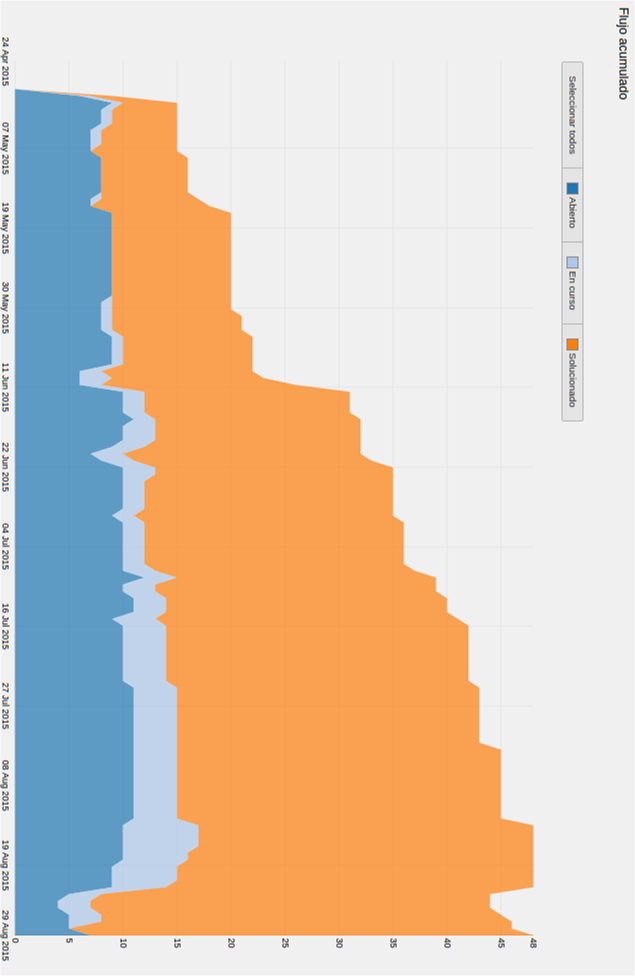
\includegraphics[scale=0.6]{figures/YouTrack/fluxoAcumulado.png}
    \caption{Gráfica do fluxo de tarefas acumulado ao longo do proxecto}
\label{fig:fluxoAcumulado}
\end{center}
\end{figure}

Por outra parte o gráfico de evolución do proxecto (figura \ref{fig:evolucionProxecto}) marcou 
durante o desenvolvemento dos sprints a liña idónea e por tanto a velocidade en relación ao ritmo
ideal. Nótese que a gráfica estima por número de tarefas e non por horas estimadas, isto 
explica as desviacións como as do mes de agosto, xa que ao dedicarse esta iteración practicamente á
memoria, a gráfica permanece estanca aínda que se sigan sumando horas de traballo de forma continua.

\begin{figure}[htp]
\begin{center}
    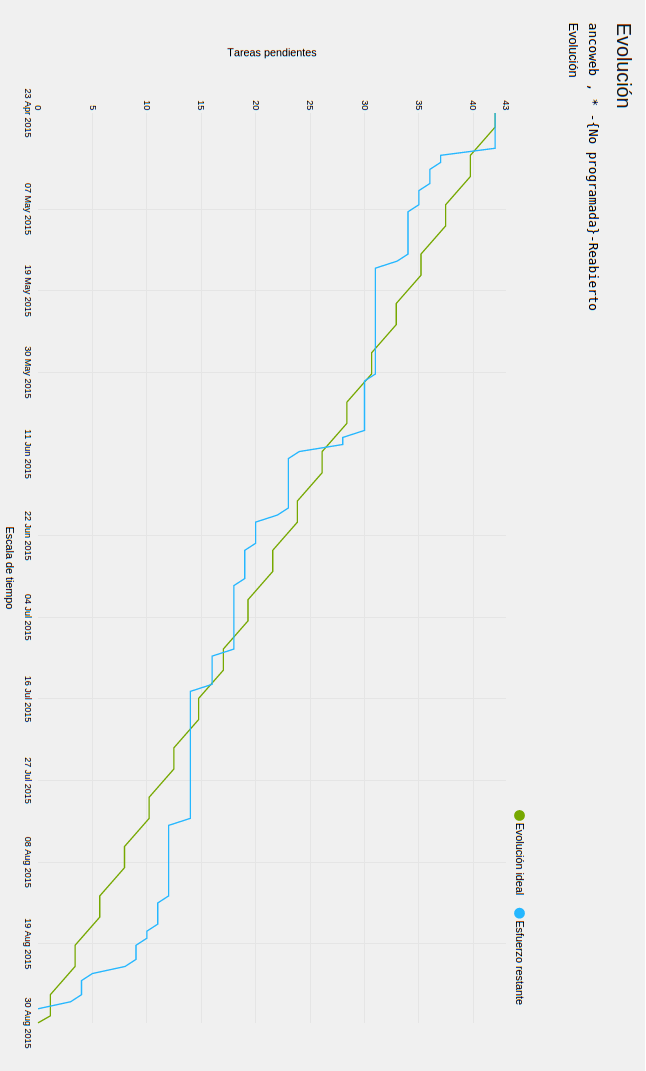
\includegraphics[scale=0.6]{figures/YouTrack/evolucionProxecto.png}
    \caption{Gráfica da evolución do proxecto}
\label{fig:evolucionProxecto}
\end{center}
\end{figure}



\begin{figure}[htp]
\begin{center}
    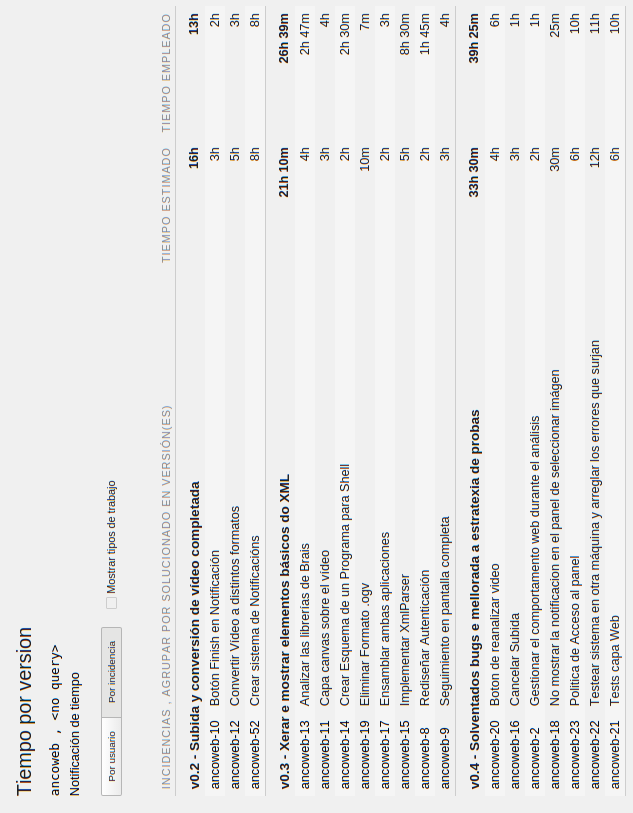
\includegraphics[scale=0.7]{figures/YouTrack/taboaHoras2_1.png}
    \caption{Táboa de horas adicadas ao proxecto por versión (1)}
\label{fig:taboaHoras2_1}
\end{center}
\end{figure}

Nas figuras\ref{fig:taboaHoras2_1} \ref{fig:taboaHoras2_2} pódense ver toda-las horas adicadas 
fronte ás horas previstas, xeralmente a predición é acertada, inda que como é lóxico non é cen por
cen exacta.

\begin{figure}[htp]
\begin{center}
    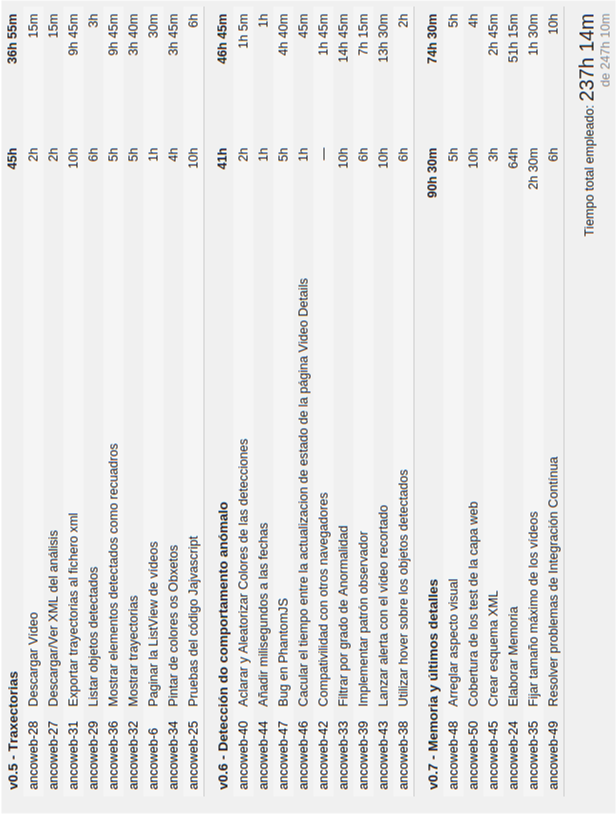
\includegraphics[scale=0.7]{figures/YouTrack/taboaHoras2_2.png}
    \caption{Táboa de horas adicadas ao proxecto por versión (2)}
\label{fig:taboaHoras2_2}
\end{center}
\end{figure}

Os datos do total de horas empregadas para a versión v1.0 suman 238 horas, que a un prezo de 
12 \euro a hora fan un custo total de 2.856,00 \euro.


% Resultados e Conclusións
\chapter{Resultados e Conclusións}

Pódese concluír por tanto, que este proxecto é unha ferramenta útil na busca áxil de novos métodos,
tanto de seguimento de obxectos como de análise de alto nivel.

O resultado ao que se chegou dista moito de ser o idóneo, pero sen ser perfecto é un avance 
significativo capaz de amosar as capacidades deste tipo de sistemas, sentando un precedente para
que nun futuro próximo se siga a mellorar esta aplicación de cara a dar visibilidade a estes 
traballos de investigación que moitas veces teñen tan complicado amosar a potencia dos seus 
resultados.

\chapter{Liñas Futuras}
\label{sec:linhasFuturas}
    En canto ás liñas futuras da aplicación, estas están compostas en parte por incidencias do 
    Product Backlog que por falta de tempo ou por ter unha baixa prioridade quedaron como tarefas 
    abertas no sitema de Xestión de Incidencias, e tamén en parte por outras funcionalidades que se
    consideran de interese no futuro pero que en ningún momento chegaron a entrar no Product Backlog
    polas súas esixencias en tempo.
    
    \section{Incidencias rexistradas como abertas ou re-abertas en YouTrack}
    
    \begin{itemize}
     \item \textbf{Cambiar as sentencias Popen shell='TRUE':}     
        Popen é unha clase empregada dende o código python do servidor para executar dende a 
        terminal unha acción determinada, pero ao executar co parámetro shell=TRUE, a información
        de se se produciu algún erro perdese. Deberíase empregar co modo shell=TRUE inda que isto
        require de varias adaptacións no código.
     \item \textbf{Internacionalización:}
        Estaría ben traducir a aplicación a Español e Galego.
     \item \textbf{Cancelar Subida:}
        Actualmente existe un bug que non permite cancela unha subida mentres esta está en proceso,
        o problema está asociado ao uso de thread's debido ao acceso a Base de datos.
     \item \textbf{Modificar o algoritmo de actualización da barra de progreso:}
        En un futuro, deberíase modificar o algoritmo de progreso de unha notificación de subida para intentar
        minimizar o número de consultas AJAX ao servidor, de xeito que se incremente o retardo entre peticións
        cando o avance de barra de progreso sexa lento e se acelere este cando o avance sexa veloz.
    \item \textbf{Mostrar Potencial:}
        Unha funcionalidade futura sería a de mostrar en cada momento cales son os puntos polo que 
        pasan mais obxectos, isto está almacenado no sistema de recoñecemento como unha matriz que 
        contén o potencial de cada punto da imaxe, e a tarefa consistiría en amosar estes potenciais
        nunha capa de información superposta ao vídeo.
    \item \textbf{Mostrar velocidade:}
        Mostrar a velocidade de cada un dos obxectos en escena así como permitir filtrar por un 
        límite de velocidade ao igual que se fai co comportamento anómalo.
    \item \textbf{Cobertura dos test da capa web:}
        Esta tarefa foi desprazada a unha rama a parte, xa que o esforzo para a súa configuración é
        cuantioso e dada a súa baixa prioridade non se chegou a completar. A solución pasa por 
        empregar algunha ferramenta como blanketJS que recolla a cobertura en phantoJS, e logo 
        enviar esta ao servidor de coveralls. 
    \item \textbf{Error ao subir dous vídeos simultaneamente}
        Revisar esta casuística na que se soben dous vídeos simultaneamente pois en certos momentos
        parece ter un comportamento erróneo.
    \item \textbf{Illar Tracking da análise de alto nivel}
        De cara a facilitar a investigación estaría ben poder realizar solo o análise de alto nivel 
        proporcionando a lista de deteccións, ou simplemente empregar unha análise de baixo nivel 
        para detectar obxectos.
    \item \textbf{Engadir compatibilidade con IE}
        Actualmente a aplicación non é compatible con Internet Explorer, en un futuro estaría ben 
        soportar este navegador.
    \end{itemize}

    
    \section{Outras funcionalidades de interese}
    
        \subsection{Vídeo en Directo}
            De cara a un futuro a funcionalidade mais desexada é a de facer o análise en directo 
            empregando o vídeo procedente dunha cámara. Pero isto prantexa unha serie de retos 
            importantes como é a sincronización do vídeo co tempo de análise ou o envío dos datos desta 
            análise á capa web, xa que isto rompe co modelo HTTP de peticións a un servidor.
            
            A solución para o problema da sincronización entre o vídeo e o tracking, pasa por retardar o
            envío do vídeo unha determinada cantidade de tempo, suficiente como para que se procese e se
            faga a análise.
            
            Non obstante como o tempo de análise non se pode prever de forma exacta, habería
            necesariamente que facer axustes para que cando a análise fose mais veloz que a reprodución
            do vídeo, a capa web mantese un buffer cos resultados recibidos e os amosase no momento 
            correcto. E por outra parte se o vídeo evolucionase mais rápido que a análise, o lado 
            servidor debería reducir o número de fotogramas a analizar descartando por exemplo un de
            cada dous ou de cada tres fotogramas.
            
            Para o problema do envío dos datos á capa web, o mais lóxico podería ser empregar unha 
            modificación do protocolo RTSP (Real-Time Streaming Protocol) visto na sección 
            \ref{sec:streaming}, de xeito que por un lado se envíe o vídeo en directo, e por outra parte
            toda a información precisa para a súa reprodución mais os datos en XML sobre as deteccións.
        
        \subsection{Panel de Control}
            Se se chegase a desenvolver un módulo que permita streaming de vídeo en directo sería de
            gran interese ter un panel no que se poidan visualizar as imaxes procedentes de 
            distintas cámaras simultaneamente. Inda que isto tamén podería facerse integrando a 
            aplicación con algunha outra aplicación de vídeo-vixilancia open-source como as citadas 
            no apartado \ref{sec:video-vixilancia-libre}
  
  
  
  
  
  
  
  
  
  


% Apéndices
\appendix

\chapter{Apéndice}

% \section{Lista de Acrónimos}

\begin{itemize}
 \item {IDE}
 \item {BD}
\end{itemize}


% TODO \section{Manual de Usuario}

% TODO \section{Manual de referencias Técnicas}

\section{Notas acerca da Terminoloxía}
	% SCRUM
\begin{itemize}
	\item{Scrum Team}
	\item{Product Owner}
	\item{Development Team}
	\item{Scrum Master}
	\item{Spring}
	\item{Sprint Planning Meeting}
	\item{Sprint Goal}
	\item{Daily Scrum}
	\item{Sprint Review}
	\item{Sprint Retrospective}
	\item{Product Backlog}
	\item{Sprint Backlog}
	
	%Outros
	
\end{itemize}
 


% Definimos el encabezado y pie de página
\fancyhead{}
\fancyhead[LE,RO]{\thepage}
\fancyhead[LO,ER]{\rightmark}

% Glosario de términos
%\printglossary


% Bibliografía
\bibliographystyle{pfc-fic}
\bibliography{biblio}

\end{document}
